\documentclass[11pt, a4paper]{book}



\usepackage{latexsym}
\usepackage{float}
\usepackage[pdftex]{graphicx}
\usepackage{amsmath}
\usepackage{amssymb}
\usepackage{textcomp}
\usepackage{color}
\usepackage{subfig}
\usepackage{caption}
\usepackage{enumerate}
\usepackage{natbib}
%\usepackage{showkeys}
\usepackage{float} 
\usepackage{longtable}
\usepackage{listings}
\usepackage{xcolor}
\usepackage{setspace}
%\usepackage[hmargin=3cm]{geometry}

\usepackage{hyperref}


\captionsetup{figurename=Fig., 
                          labelfont=it, 
                          textfont=small,
                          labelsep=period
                          }
                          
                                                 
% clickable page number
%\hypersetup{linktocpage,

% clickable content
\hypersetup{bookmarks=true,
                       colorlinks=true,
                       linkcolor=black,
                       urlcolor=blue,
                       citecolor=black
                       }




\newtheorem{theorem}{Theorem}[section]
\newtheorem{lemma}[theorem]{Lemma}
\newtheorem{corollary}[theorem]{Corollary}
\newtheorem{proposition}[theorem]{Proposition}
\newtheorem{definition}[theorem]{Definition}
\newtheorem{problem}[theorem]{Problem}
\newtheorem{example}[theorem]{Example}
\newtheorem{construction}[theorem]{Construction}
\newtheorem{conjecture}[theorem]{Conjecture}
\newtheorem{remark}[theorem]{Remark}
\newtheorem{question}[theorem]{Question}
\newtheorem{algorithm}[theorem]{Algorithm}
\newtheorem{comment}[theorem]{Comment}
\newtheorem{observation}[theorem]{Observation}
\newtheorem{hypothesis}[theorem]{Hypothesis}
\newtheorem{claim}[theorem]{Claim}

\input amssym.def
\input amssym.tex

\long\def\delete#1{}

\newcommand{\HRule}{\rule{\linewidth}{0.5mm}}

\def\proof{\par\noindent{\bf Proof~}}
\def\Proof{\par\noindent{\bf Proof of Theorem~}}
%\def\qed{\ifmmode\square\else\nolinebreak\hfill$\square$\fi\par\vskip12pt}
\def\qed{\hfill$\Box$\vspace{12pt}}

\def\ov{\overline}
\def\la{\langle}
\def\ra{\rangle}
\def\tr{{\rm tr}}
\def\div{\,\Big|\,}
\def\notdiv{\,{\not\Big|}\,}

\def\BBB{\Bbb B}
\def\CCC{\Bbb C}
\def\FFF{\Bbb F}
\def\ZZZ{\Bbb Z}
\def\NNN{\Bbb N}
\def\SSS{\Bbb S}

\def\AA{{\cal A}}
\def\BB{{\cal B}}
\def\CC{{\cal C}}
\def\DD{{\cal D}}
\def\EE{{\cal E}}
\def\FF{{\cal F}}
\def\GG{{\cal G}}
\def\JJ{{\cal J}}
\def\KK{{\cal K}}
\def\LL{{\cal L}}
\def\NN{{\cal N}}
\def\PP{{\cal P}}
\def\QQ{{\cal Q}}
\def\RR{{\cal R}}
\def\SS{{\cal S}}
\def\TT{{\cal T}}
\def\XX{{\cal X}}
\def\VV{{\cal V}}
\def\II{{\cal I}}
\def\HH{{\cal H}}


\def\Q{{\rm Q}}
\def\D{{\rm D}}
\def\A{{\rm A}}
\def\B{{\rm B}}
\def\C{{\rm C}}
\def\F{{\rm F}}
\def\P{{\rm P}}
\def\R{{\rm R}}
\def\S{{\rm S}}
\def\L{{\rm L}}
\def\I{{\rm I}}
\def\J{{\rm J}}
\def\M{{\rm M}}

\def\bfA{{\bf A}}
\def\bfB{{\bf B}}
\def\bfC{{\bf C}}
\def\bfD{{\bf D}}
\def\bfE{{\bf E}}
\def\bfL{{\bf L}}
\def\bfN{{\bf N}}
\def\bfZ{{\bf Z}}
\def\bfO{{\bf O}}
\def\bfP{{\bf P}}
\def\bfQ{{\bf Q}}
\def\bfS{{\bf S}}
\def\bfT{{\bf T}}

\def\b0{{\bf 0}}
\def\ba{{\bf a}}
\def\bb{{\bf b}}
\def\bc{{\bf c}}
\def\bd{{\bf d}}
\def\be{{\bf e}}
\def\bi{{\bf i}}
\def\bj{{\bf j}}
\def\bk{{\bf k}}
\def\bx{{\bf x}}
\def\by{{\bf y}}
\def\bz{{\bf z}}
\def\bs{{\bf s}}
\def\bt{{\bf t}}
\def\bu{{\bf u}}
\def\bv{{\bf v}}
\def\bw{{\bf w}}

\def\De{\Delta_{2}(T)}
\def\Ga{\Gamma}
\def\La{\Lambda}
\def\Si{\Sigma}
\def\Om{\Omega}
\def\The{\Theta}


\def\a{\alpha}
\def\b{\beta}
\def\d{\delta^*(T)}
\def\g{\gamma}
\def\lamh11{\lambda_{h,1,1}}
\def\s{\sigma}
\def\t{\tau}
\def\ve{\varepsilon}
\def\vp{\varphi}
\def\p{\psi}

%%%%%%% my own short cut %%%%%%%%%%%%
\def\uij{u_{0\dots ij}}
\def\uijk{u_{0\dots ijk}}
\def\ujk{u_{0\dots jk}}
\def\ujkl{u_{0\dots jkl}}
\def\lnu{f(N(u_1))}
\def\lcu{f(C(u_0))}
\def\lcuu{f(C(u_1))}
\def\gnu{g(N(u_1))}
\def\gcu{g(C(u_0))}
\def\gcuu{g(C(u_1))}


\def\tmk{T_{m,k}}
\def\tm2{T_{m,2}}
\def\lamh11{\lambda_{h,1,1}}
\def\lhpq{L(h,p,q)}
\def\chpq{C(h,p,q)}
\def\lamhpq{\lambda_{h,p,q}}
\def\thpq{\t_{h,p,q}}
\def\th11{\t_{h,1,1}}
\def\kd{\KK_{2\Delta}}
\def\kdd{\KK_{2\Delta-1}}

%%%%%%%%%%%%%%%%%%%%%%%%%%%%%



\def\Alt{{\rm Alt}}
\def\Sym{{\rm Sym}}
\def\Inn{{\rm Inn}}
\def\Out{{\rm Out}}
\def\Cay{{\rm Cay}}
\def\Aut{{\rm Aut}}
\def\aut{{\rm aut}}
\def\soc{{\rm soc}}
\def\wr{{\rm\,wr\,}}
\def\Diag{{\rm Diag}}
\def\Syl{{\rm Syl}}
\def\PSL{{\rm PSL}}
\def\PGL{{\rm PGL}}
\def\PSU{{\rm PSU}}
\def\PGU{{\rm PGU}}
\def\SU{{\rm SU}}
\def\SL{{\rm SL}}
\def\GL{{\rm GL}}
\def\AGL{{\rm AGL}}
\def\PGL{{\rm PGL}}
\def\AG{{\rm AG}}
\def\PG{{\rm PG}}
\def\GF{{\rm GF}}
\def\CR{{\rm CR}}
\def\GammaL{{\rm\Gamma L}}
\def\AGammaL{{\rm A\Gamma L}}
\def\PGammaL{{\rm P\Gamma L}}
\def\PGammaU{{\rm P\Gamma U}}
\def\U{{\rm U}}
\def\PSp{{\rm PSp}}
\def\Sp{{\rm Sp}}
\def\PO{{\rm P\Omega}}
\def\POmega{{\rm P\Omega}}
\def\E{{\rm E}}
\def\F{{\rm F}}
\def\G{{\rm G}}
\def\Sz{{\rm Sz}}
\def\Ree{{\rm Ree}}

\def\McL{{\rm McL}}
\def\Ru{{\rm Ru}}
\def\Ly{{\rm Ly}}
\def\Co{{\rm Co}}
\def\Fi{{\rm Fi}}
\def\Th{{\rm Th}}
\def\BM{{\rm BM }}
\def\ON{{\rm O'N}}
\def\HS{{\rm HS}}
\def\Suz{{\rm Suz}}
\def\He{{\rm He}}
\def\Co{{\rm Co}}
\def\HN{{\rm HN}}
\def\HA{{\rm HA}}
\def\AS{{\rm AS}}
\def\TW{{\rm TW}}
\def\PA{{\rm PA}}

\def\arc{{\tt arc}}
\def\Arc{{\tt Arc}}
\def\AF{{\rm AF}}
\def\CR{{\rm CR}}
\def\TCR{{\rm TCR}}
\def\girth{{\rm girth}}
\def\Sim{{\tt Simple}}
\def\val{{\tt val}}
\def\fix{{\rm fix}}
\def\det{{\rm det}}
\def\gcd{{\tt gcd}}
\def\diag{{\rm diag}}
\def\Ker{{\rm Ker}}

\def\cc{{$C_{p_{1}, p_{2}, p_{3}}$}}
\def\ch{{$C_{p_{1}, p_{2}, p_{3}}(H)$}}


\usepackage{fancyhdr}

\pagestyle{fancy}
\renewcommand{\chaptermark}[1]{\markboth{#1}{}}
\renewcommand{\sectionmark}[1]{\markright{\thesection\ #1}}
\fancyhf{}
\fancyhead[LE,RO]{\bfseries\thepage}
\fancyhead[LO]{\bfseries\rightmark}
\fancyhead[RE]{\bfseries\leftmark}
\renewcommand{\headrulewidth}{0.5pt}
\renewcommand{\footrulewidth}{0pt}
\addtolength{\headheight}{0.5pt}
\setlength{\footskip}{0in}
\renewcommand{\footruleskip}{0pt}
\fancypagestyle{plain}{%
 \fancyhead{}
 \renewcommand{\headrulewidth}{0pt}
}


\newcommand{\mymargin}[1]{\marginpar{\textcolor{cyan}{#1}}}

\parskip 0.05in
 
\begin{document}
\onehalfspacing
\begin{titlepage}

\begin{center}


% Upper part of the page

\textsc{\LARGE University of Melbourne}\\
{\large Department of Mathematics and Statistics}\\[1.5cm]

\textsc{\Large Master Thesis}\\[0.5cm]


% Title
\HRule \\[0.4cm]
{ \LARGE  \bf Solving distance three linear and cyclic metric labelling problems of complete $m$-ary trees }\\[0.4cm]

\HRule \\[1.5cm]


% Author and supervisor
\begin{minipage}{0.4\textwidth}
\begin{flushleft} \large
\emph{Author:}\\
Yang \textsc{Li}
\end{flushleft}
\end{minipage}
\begin{minipage}{0.4\textwidth}
\begin{flushright} \large
\emph{Supervisors:} \\
Associate Professor Sanming \textsc{Zhou}\\
Dr. Deborah \textsc{King}
\end{flushright}
\end{minipage}

\vfill


% Bottom of the page
{\large October 28, 2011}

\end{center}

\end{titlepage}
 
\frontmatter
 

 \chapter*{\centering Abstract}
\addcontentsline{toc}{chapter}{Abstract}

The channel assignment problem is concerned with assigning a channel to each of a set of transmitters such that the maximum span of the channels is minimized under some distance constraints. Given $p_1, p_2, p_3, \dots$ all positive integers, an $L(p_1, p_2, p_3,\dots)$-labelling of a graph is an assignment of non-negative integers to its vertices such that vertices at distance $i$ apart must receive labels with separation at least $p_i$. The span of such a labelling is the difference between the maximum and minimum labels used. The objective is to find the minimum span over all $L(p_1, p_2, p_3, \dots)$-labellings of the graph. 

In this paper, we focus on $L(h,p,q)$-labellings of complete $m$-ary trees. We prove that the minimum span of the $\lhpq$-labelling of complete $m$-ary trees is an exact value. In the second part of this thesis, we introduce another labelling system the $C(p_1,p_2,p_3, \dots)$-labelling, called the cyclic metric labelling. We prove that the minimum span of the $C(h,1,1)$-labelling of complete $m$-ary trees is also an exact value, but this time it is dependent upon the parameter $m$ and $h$. 


%\begin{romanpages}          % start roman page numbering
\tableofcontents            % generate and include a table of contents
\listoffigures              % generate and include a list of figures
%\end{romanpages}            % end roman page numbering


\mainmatter
%\openup 0.5\jot \maketitle


% content starts
\chapter{Introduction}

This thesis studies various graph labelling problems over a collection of some interesting trees. 

In real world, when assigning channels to transmitters at different locations, certain rules are applied for a various of practical reasons. One of the major concern is o avoid interference when doing so. This requires large separation for two transmitters located close to each other. Bandwidth is a limited resource in real world. The larger a bandwidth is, the more money it will cost when setting up channels. The objective of channel assignment problem is to keep the bandwidth as small as possible while no interference occurs in a set of transmitters. 

Channel assignment problems were formulated by graph theorists into graph labelling problems in order to solve real world problems more accurate. This not only introduce an interesting area of research into mathematical world, but also saves resources, time and money in practice. In details, channel assignment problems can be represented by graph labelling problems, where vertices of a graph represent a set of transmitters and the non-negative integer labels for vertices represent the channel assigned to each of a set of transmitters. The aim of solving graph labelling problems becomes minimising the maximum used label. In this thesis, we will focus on two such problems, namely the linear and cyclic metric labelling problems. 

The linear metric labelling, normally denoted by $L(p_1, p_2, p_3, \dots)$, is an assignment $f: V(G) \rightarrow \{0, 1, 2, \dots, k\}$ of non-negative integers to vertices of a graph $G$ such that two vertices at distance $i$ apart must receive labels with separation at least $p_i$, where $p_i$ is the $i^{th}$ parameter of the $L(p_1, p_2, p_3, \dots)$-labelling. The difference between the maximum value and the minimum value of labels used is called the span of such a map. The aim of the $L(p_1, p_2, p_3, \dots)$-labelling problem is to find the smallest $k \in \mathbb{Z}_{\ge 0}$, which is called the minimum span of the $L(p_1, p_2, p_3, \dots)$-labelling of the graph $G$, which satisfies the above constraint. The $L(p_1, p_2)$-labelling problem has been widely studied. However, the $L(p_1,p_2,p_3)$-labelling problem is now attracting great interest because of its practical and theoretical interests. 

The cyclic metric labelling, denoted by $C(p_1, p_2, p_3, \dots)$, is similar to the $L(p_1, p_2, p_3, \dots)$-labelling. It is also an assignment $f: V(G) \rightarrow \{0, 1, 2, \dots, k\}$ of non-negative integers to vertices of a graph $G$. However, two vertices at distance $i$ apart now receive labels with separation at least $p_i \pmod{k}$. The aim of the $C(p_1, p_2, p_3, \dots)$-labelling problem is the same as that for the $L(p_1, p_2, p_3, \dots)$-labelling problem. That is, to find the smallest $k$ that satisfies the above constraint. Similarly, the span and the minimum span of the $C(p_1, p_2, p_3, \dots)$-labelling of the graph $G$ are both the same as the linear case. The $C(p_1, p_2, p_3, \dots)$-labelling problem has been as not broadly studied as the $L(p_1, p_2, p_3)$-labelling problem, however many good results about such a labelling have been obtained for various classes of graphs.  

We will mainly study the $L(p_1, p_2, p_3)$-labelling problem with $p_1 = h, p_2=p_3=1$. That is, the $L(h,1,1)$-labelling problem. Moreover, the collection of graphs that will be studied are the family of complete $m$-ary trees and its extensions. A complete $m$-ary tree is a tree $T$ such that every vertex of $T$, except its leaves, has exactly $m$ children. The reason why we choose to work on complete $m$-ary trees is because every tree is a subtree of a complete $m$-ary tree. Thus if we can find a tight upper bound for the family of complete $m$-ary trees, then this bound is also an upper bound for all trees. 

We begin by introducing some basic concepts in graph theory that will be used in this thesis. Chapter 3 focuses on the $L(h,1,1)$-labelling problem. We start off by giving some definitions and notations. Then we will review some known results of linear metric labelling problem for different types of graphs. Our results come in the following two sections. In Section 3.4, we prove the minimum span of the $L(h,1,1)$-labelling of complete $m$-ary trees to be $2m+h-1$ for height $2$ complete $m$-ary trees; $2m+h$ for height $3$ complete $m$-ary trees. Then in the next section, this result is extended to the $\lhpq$-labellings of complete $m$-ary trees. In Section 3.6, we further extended the $\lhpq$-labelling results to some larger families of trees, which contain the set of complete $m$-ary trees as a subset. 

In Chapter 4, we turn our attention to $C(h,1,1)$-labelling problem. The structure of Chapter 4 is the same as the structure of Chapter 3. We start off by introducing new definitions and notations. We then review some known results for cyclic metric labelling problems. Then in Section 4.3, we give our own results of the $C(h,1,1)$-labelling of complete $m$-ary trees as well as detailed proofs. Instead of an exact value, this time the results are two values, which depend on the number of children $m$ and the first parameter $h$. Precisely, the minimum span of the $C(h,1,1)$-labelling is $\max\{2m+h-1, 2h+m-1\}$ for height $2$ complete $m$-ary trees; $\max\{2m+h, 2h+m-1\}$ for height $3$ complete $m$-ary trees. In the next section, these results are extended to the $\chpq$-labelling of complete $m$-ary trees. We find a reasonable bound for complete $m$-ary trees with height $2$. For height $3$ complete $m$-ary trees, we only give an estimation of the upper bound. In Section 4.5, we again focus on those families of trees that we considered in Section 3.6. However, we only generalise the $C(h,1,1)$-labelling of these trees. 

Chapter 5 is a short conclusion of our results in this thesis. We also give a plan for some further studies in future. 

In the appendix, there is a table of notations that are widely used throughout this thesis. 









\chapter{The Basics}
\section{Graphs and subgraphs}

In this chapter, we will introduce to the reader some basic definitions and notation in graph theory, which will be used throughout this thesis. We will follow \citeauthor{diestel00}'s book \textit{Graph Theory} for these standard definitions and notation.

Now, let us start with the definition of a graph. Informally, a \textit{graph} is a set of vertices and edges, where the edges connect some of the vertices in the set. The letter $u$ and $v$ are the most commonly used notation for vertices, and $e$ is also commonly used to denote an edge of a graph, where in this case the two vertices connected by the edge $e$ is unspecified. We say a vertex $v$ is incident to an edge $e$ if $e$ is an edge at $v$. We also denote the edge $e$ by $uv$ if the vertices $u$ and $v$ are both incident to $e$. In this case $u$ and $v$ are called the {\it {ends}} of the edge $e$. We now give a more precise definition of a graph. A {\it{graph}} is an ordered pair $G = (V(G), E(G))$, where $V(G)$ and $E(G)$ denote the sets of  vertices and edges of the graph $G$ respectively. We say a graph is a \emph{simple graph} if it does not contain a loop between a pair of vertices. The following are two examples of graphs. In the first case (Fig. \ref{graph} (a)), the graph is connected (contains only one component), while in the second case (Fig. \ref{graph} (b)), the graph is disconnected. A formal definition of a connected graph will be given in the next section. 
\begin{figure}
  \centering
     % \vspace{-10pt}
    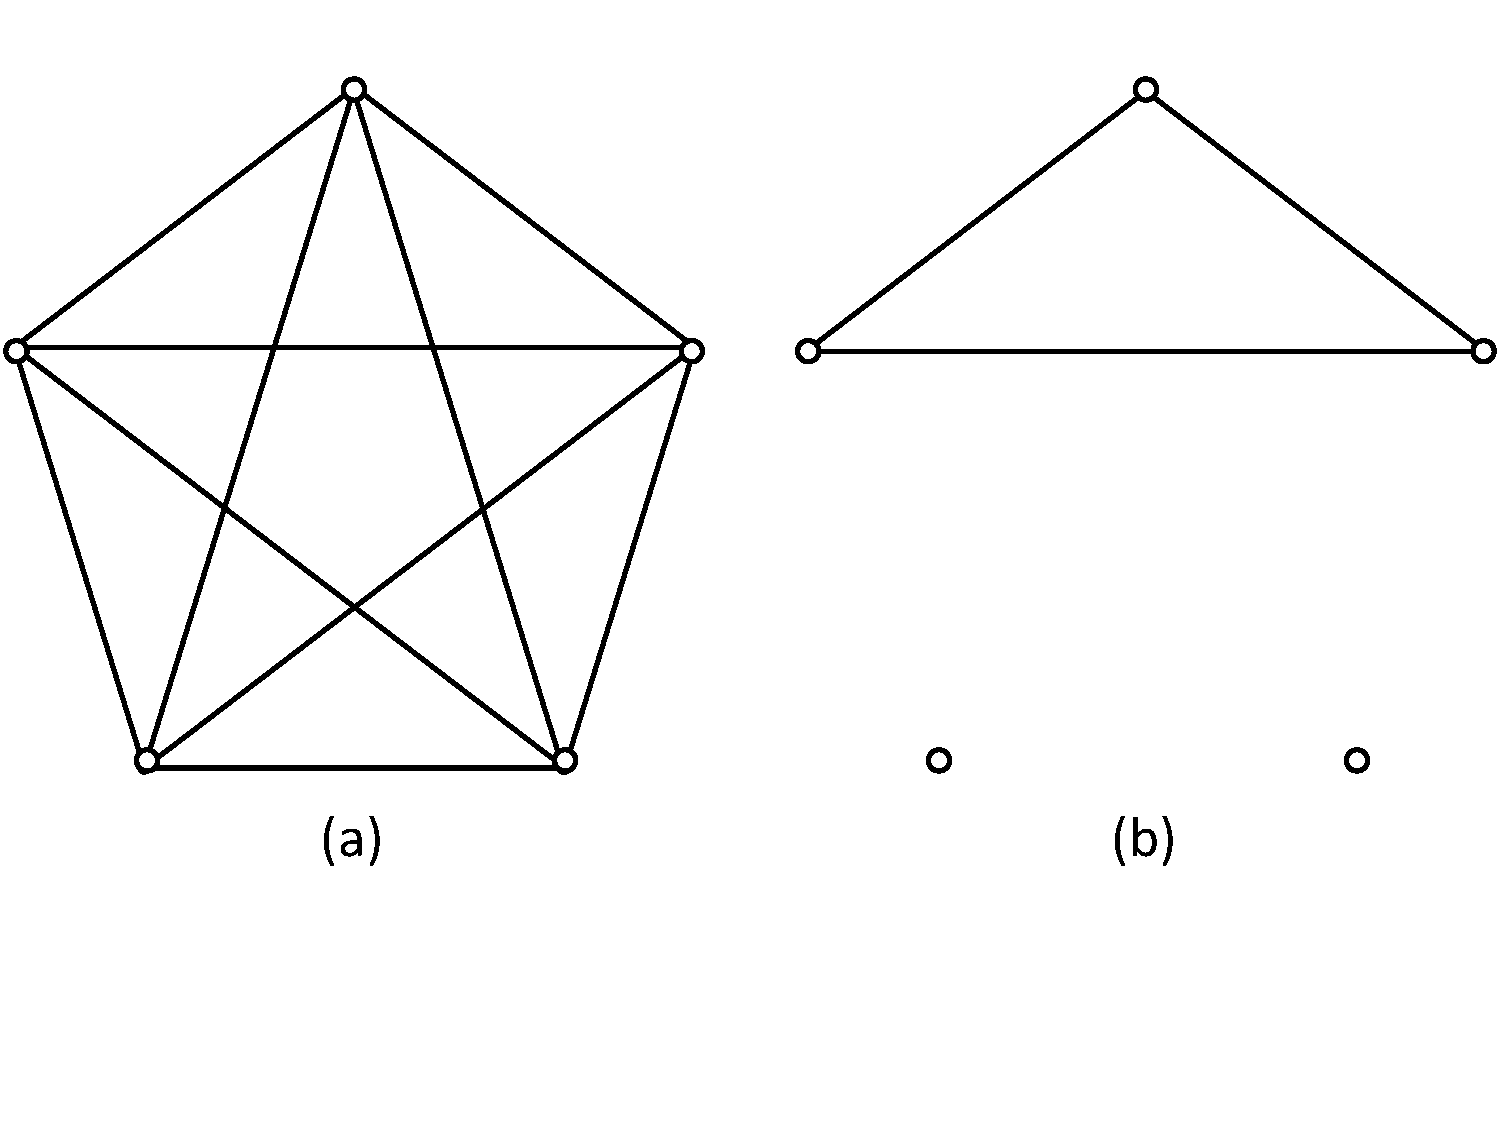
\includegraphics[scale=0.35]{../figures/fig2-1.pdf}
        \vspace{-30pt}
  \caption{Example of graphs}
  \label{graph}
\end{figure}

Since $V(G)$ and $E(G)$ denote the sets of vertices and edges of the graph $G$, there must be subsets of $V(G)$ and $E(G)$. This brings in the following definition. A graph $G' = (V'(G), E'(G))$ is a {\it{subgraph}} of a graph $G = (V(G), E(G))$ if $V'(G) \subseteq V(G)$ and $E'(G) \subseteq E(G)$ are subsets. We use $G' \subseteq G$ to denote $G'$ is a subgraph of $G$. Sometimes we also say that the graph $G$ contains $G'$ as a subgraph.  For the two graphs below (Fig \ref{graph}), clearly (b) is a subgraph of (a). 

The {\it{degree}} of a vertex $v$ in a graph $G$ is the number of vertices adjacent to $v$. It is denoted by $d_G(v)$ or $d(v)$.\footnote{This notation, as well as others, are widely used throughout this thesis. For convenience, we drop the index $G$ if $G$ is clearly understood.}  Equivalently, it can be defined as the number of edges incident to $v$. In Fig \ref{graph} (b), the bottom left vertex has degree $0$. The top  vertex has degree $2$. Sometime we use $\Delta(G)$ (or just $\Delta$) to denote the maximum degree of a graph $G$. Precisely, $\Delta(G) := \max_{u \in V(G)} d(u)$. 


%%%%%%%%%%%%%%%%%%%%%%%%
\section{Paths, cycles and trees}
Intuitively, a path is a finite series of edges between a pair of vertices. To make it more formal, we define a {\it {path}} $P = (V, E)$ as a subgraph of a simple graph $G$, where the set $V = \{x_0, x_1, \dots, x_n\}$ and the set $E = \{x_0x_1, x_1x_2, \dots, x_{n-1}x_n\}$. The {\it{length}} of $P$ is said to be the number of edges in $P$. A path $P$ of length $n$ is normally denoted by $P^n$. Notice that for vertices $x_0$ and $x_n$ of a graph, there could be more than one path between them. Hence we use $P = x_0x_1\dots x_{n-1}x_n$ referring to the particular path that we are interested in. We call a path $P$ from $x_0$ to $x_n$ that has the least length the {\it{shortest path}} between $x_0$ and $x_n$. Though the length of such a path is the least among all other paths from $x_0$ to $x_n$, the shortest path between $x_0$ and $x_n$ is not unique in some graphs. We use the length of the shortest path between two vertices $x_0$ and $x_n$ to define the {\it{distance}} between $x_0$ and $x_n$ in a graph $G$, denoted by $dis_G(x_0,x_n)$ or $dis(x_0,x_n)$ or $d(x_0,x_n)$. On the other hand, the \textit{diameter} of a graph $G$, denoted by $diam(G)$ is the length of the longest path in $G$. 

We call a path with the two ends are identical a \textit{cycle}, denoted by $C = x_0x_1\dots x_nx_0$. In other words, a cycle is a closed path. The \emph{length} of a cycle is defined to be the number of vertices or edges in it. A cycle $C$ of length $n$ is said to be an {\it{$n$-cycle}} and denoted by $C^n$.

Let us use the following example to make the above definitions clear. 

\begin{example}
Let $G$ be a graph as shown in Fig. \ref{path and cycle}. Then $P = x_0x_1x_2x_3x_4$ is a path of length $4$ in $G$, and $C =  x_0x_1x_2x_3x_4x_0$ is a cycle of length $5$ in $G$. Also, the distance between $u_0$ and $u_4$ in $G$ is $1$, as there is a shortest path $u_0u_1$ of length $1$ in $G$. 

\begin{figure}
  \centering
      \vspace{-10pt}
    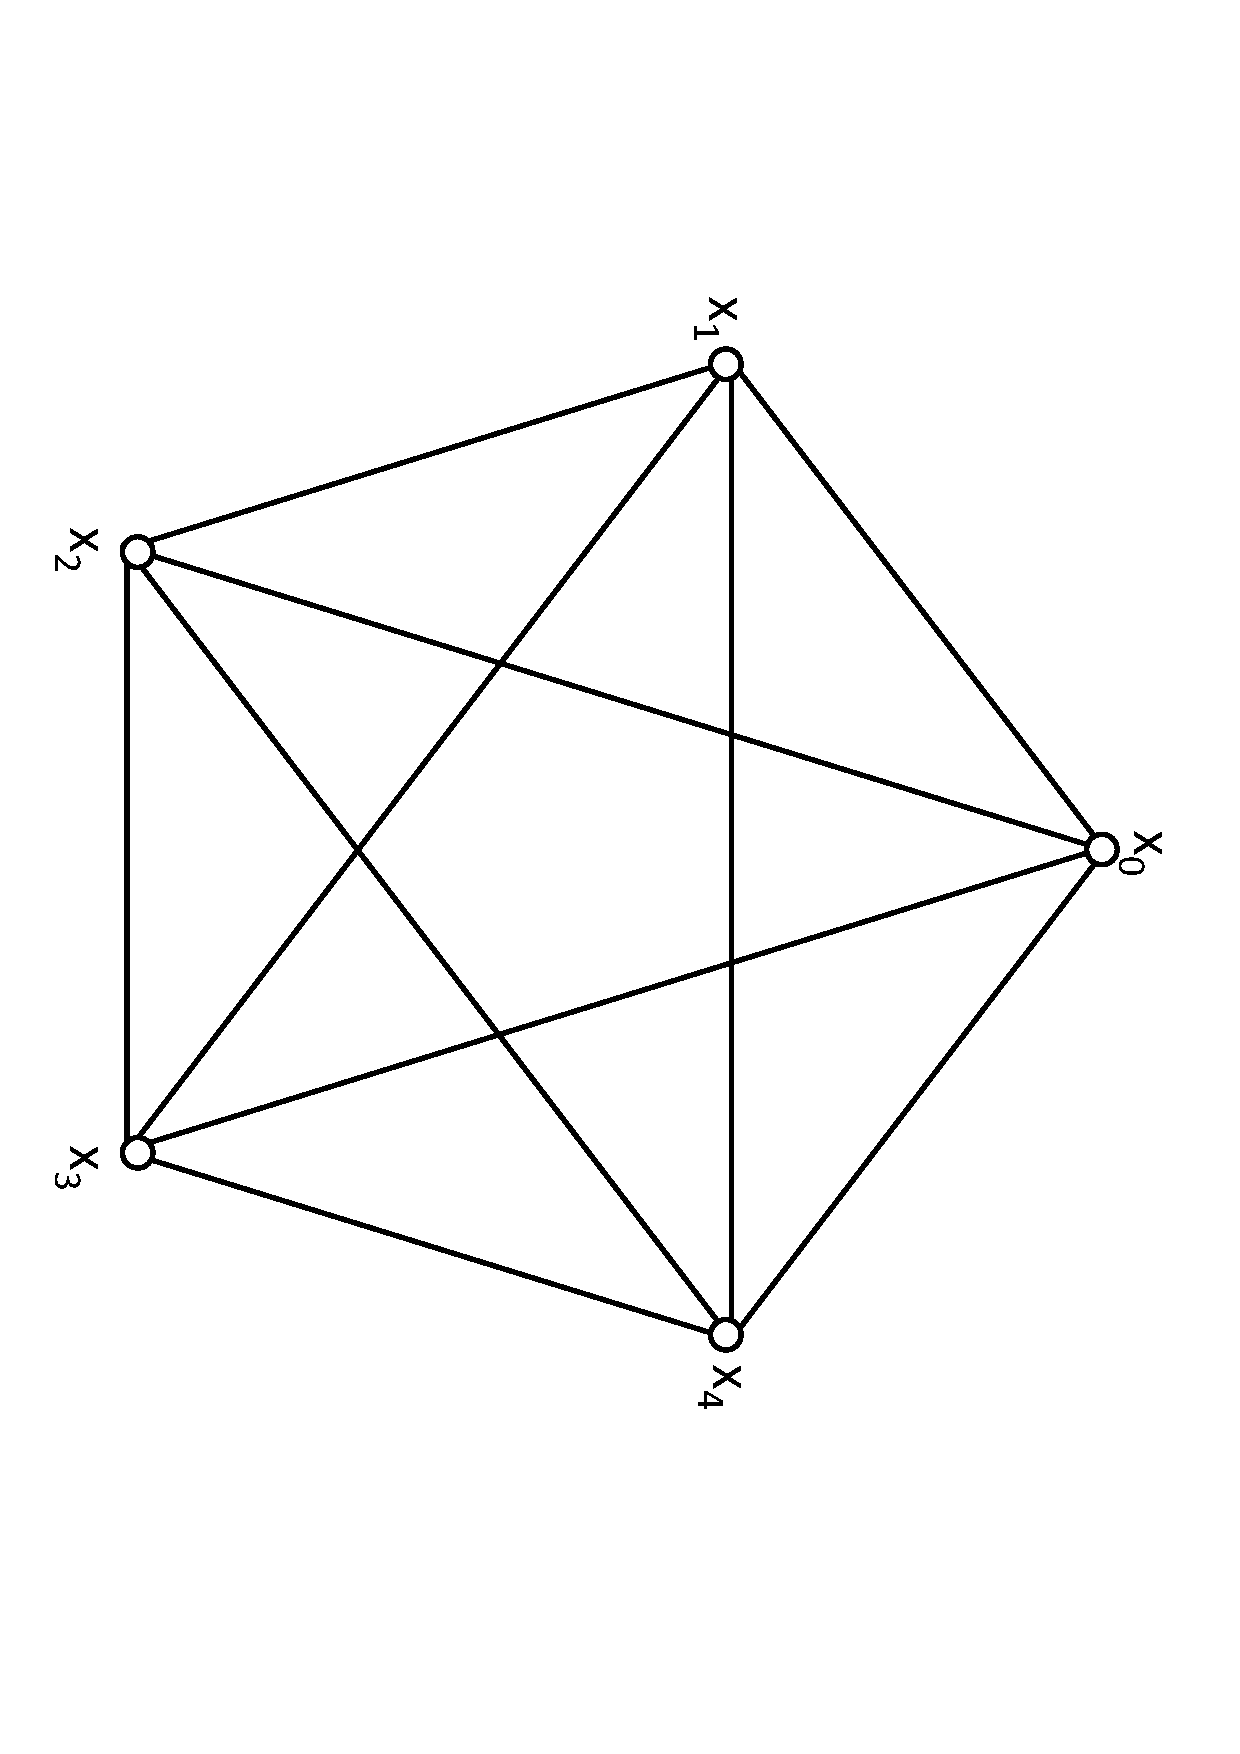
\includegraphics[scale=0.25, angle=90]{../figures/fig2-2.pdf}
        \vspace{5pt}
  \caption{Example of a path and a cycle}
  \label{path and cycle}
\end{figure}

\end{example}

Any graph $G$ may or may not contain a cycle as a subgraph. We say a graph is {\it{acyclic}} if it does not contain a cycle. 

A \emph{component} of a graph is an isolated block that is not connected to any other vertices or edges of the graph. A graph is {\it{connected}} if it has only one component. On the other hand, if a graph contains more than one component, then we say such a graph is not connected or {\it{disconnected}}. We have seen examples of connected and disconnected graphs previously (Fig \ref{graph}). 

Using the above definitions, we can give a formal definition of trees. A {\it{tree}} is defined as a connected acyclic graph. Normally, we use $T$ to denote a tree. For instance, a path is a tree. If a graph is acyclic but not connected, then it contains more than one tree. Such a graph is said to be a {\it{forest}}. When dealing problems with a tree, it is convenient to have a special vertex. Such a vertex is called the \emph{root} of this tree. A tree with a fixed root is called a {\it{rooted tree}}. Notice that we can only make one special vertex in each tree. In other words, there is only one root in each rooted tree. All trees that are dealt with in this thesis are rooted trees, so in future we will only say a tree $T$ instead of a rooted tree $T$ just for convenience. A {\it{leaf}} of a tree is a non-rooted vertex such that the degree of the vertex is exactly one. We say vertices of a tree $T$ are \textit{internal vertices} if they are not leaves of $T$. The root of $T$ is also an internal vertex of $T$. The {\it{parent}} of a vertex $v$ in a tree $T$ is a vertex that is connected to $v$ on the path from $v$ to the root of $T$, denoted by $P(v)$. The parent $P(v)$ in a tree $T$ is unique, since there is a unique path between any two vertices of $T$ and the parent of $v$ is on this unique path. We will prove this in the following proposition. The {\it{child}} of a vertex $v$ in $T$ is defined as a vertex that is adjacent to $v$ on the path from $v$ to a leaf of $T$, denoted by $C(v)$. Unlike the parent, a vertex $v$ can have more than one child if there is more than one leaf in $T$. 

Here, we introduce another concept, the \emph{neighbours} of a vertex $u \in V(G)$, which is the set of vertices adjacent to $u$. Precisely, we have the following definition. 

\begin{definition}
\label{neighbour}
Let $u \in V(G)$ be a vertex of a graph $G$. We define the set of neighbours of $u$ to be  
\[
N(u) := \{v \in V(G) \mid d(u,v) = 1\}.
\]
\end{definition}

Intuitively, if we have a tree, we can ask the height of such a tree. The length of the longest path from the root of $T$ to leaves of $T$ is defined to be the {\it{height}} of a tree $T$ and denote it by $hei(T)$. For any vertex $u$ in a tree $T$, we can also talk about its {\it{depth}}. It is defined as the length of the path from the root of $T$ to any vertex $u$ of $T$, denoted by $dep_T(u)$. This is well-defined because there is a unique path from the root to any vertex of $T$. Precisely, we have the following proposition. 

\begin{proposition}
\label{prop:unique path}
Let $T$ be a tree. There is a unique path between any two vertices $u, v \in V(T)$. 
\end{proposition}

\begin{proof}
The proof of this proposition is straightforward. Let $P$ be a path in the tree $T$ from $u$ to $v$. Suppose there is another path $P'$ in $T$ from $u$ to $v$ such that $P \neq P'$. Since both paths have end points $u$ and $v$, there eixsts a cycle in $T$ passes through $u$ and $v$. But $T$ is acyclic by the definition of a tree, so we must have $P=P'$.
\end{proof}
\qed

If we let $u$ to be the root of $T$, then the proposition claims there is a unique path between the root of $T$ and any other vertex in $T$. Due to the uniqueness of a path in trees, we can use $P_{uv}$ to denote the unique path from vertex $u$ to $v$ in a tree $T$ for convenience. 

\begin{example}
In Fig. \ref{height and depth}, the tree $T$ has height $4$, as $P_{uw}$ is the longest path from the root of $T$ to its leaves, and it has length $4$. Also, $dep(v) = 3$ as the length of the path $P_{uv}$ is $3$. 

\begin{figure}
  \centering
      \vspace{-10pt}
    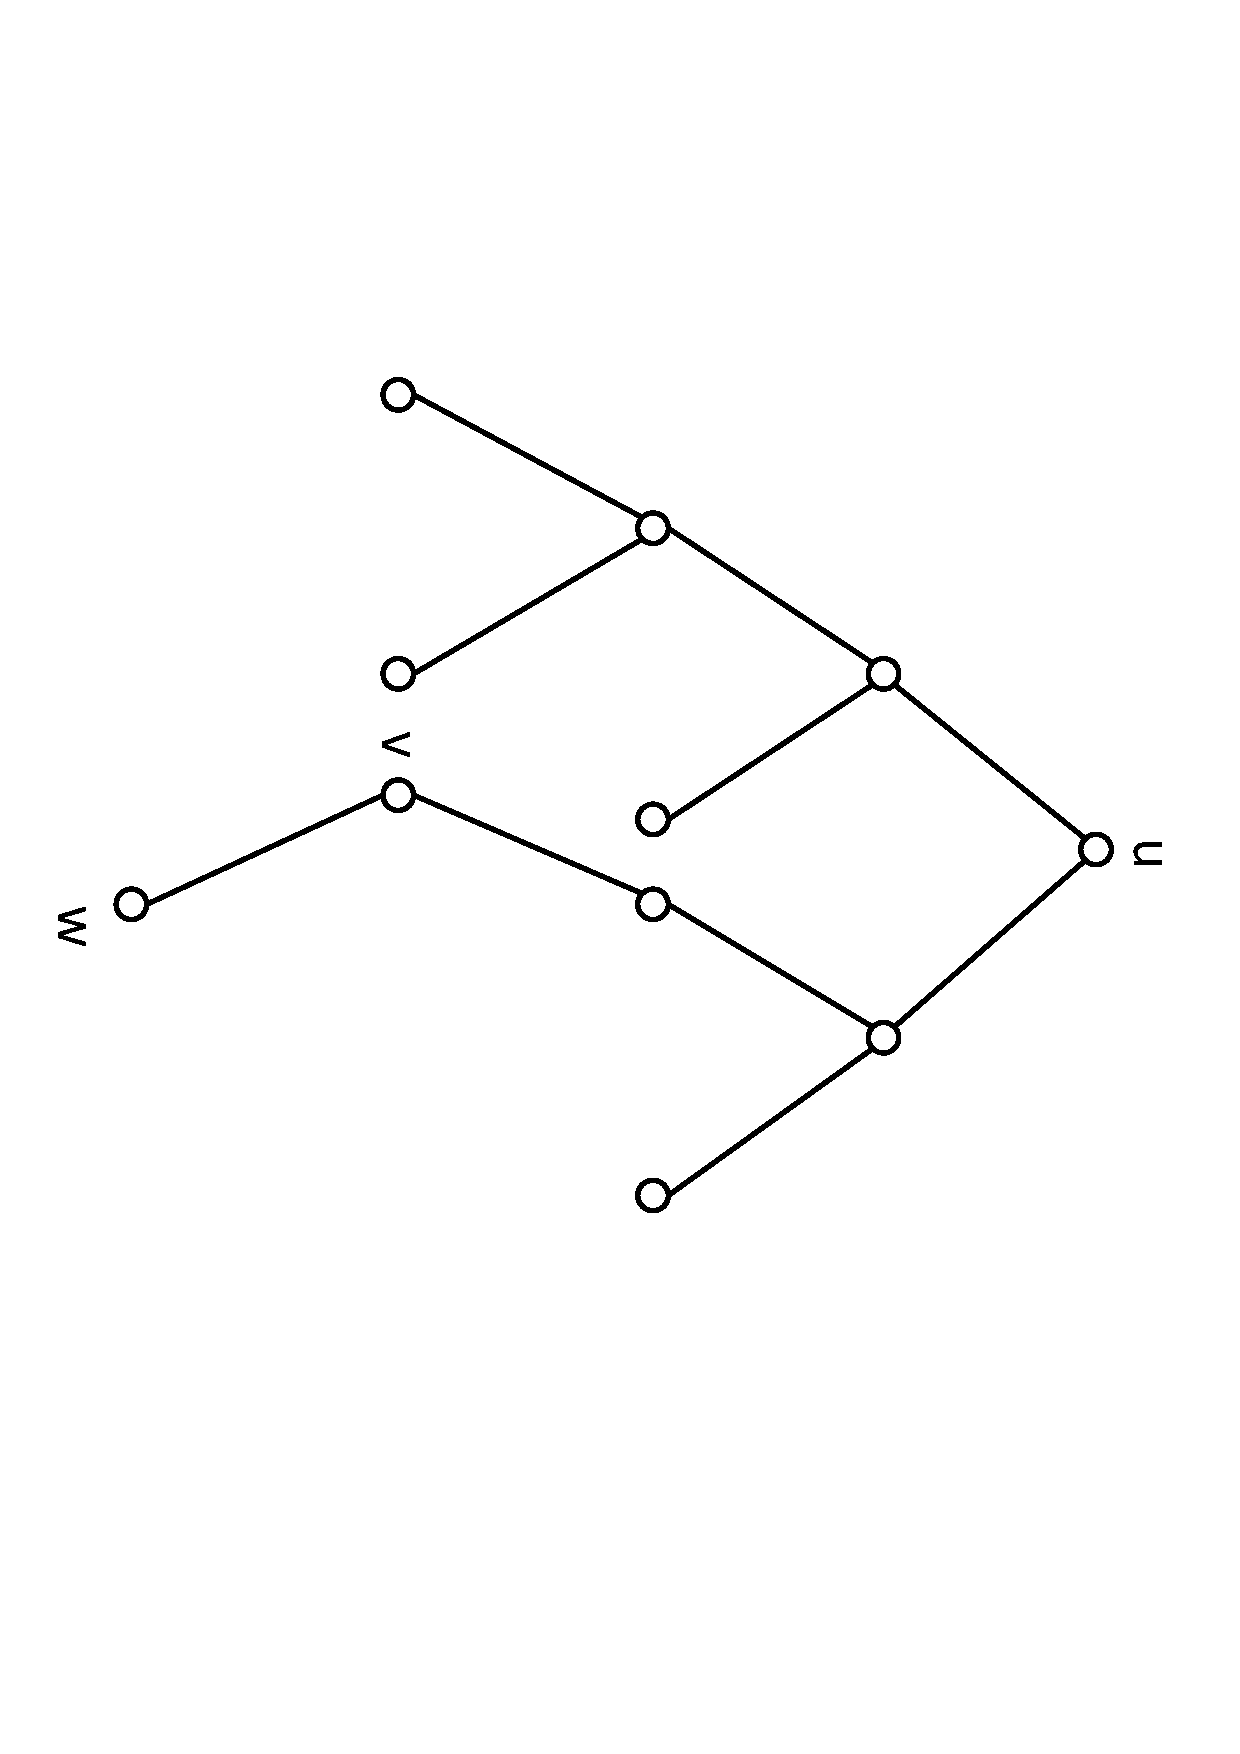
\includegraphics[scale=0.3, angle=90]{../figures/fig2-3.pdf}
        \vspace{-0pt}
  \caption{Tree height and vertex depth}
  \label{height and depth}
\end{figure}
\end{example}

%%%%%%%%%%%%%%%%%%%%%%%%%%%%%%%%%%%%%

\section{Complete $m$-ary trees}
Our research begins with labelling the set of complete $m$-ary trees. We now give the formal definition of a complete $m$-ary tree. 
\begin{definition}
\label{m-ary tree}
A tree $T$ is said to be an $m$-ary tree if every internal vertex  of $T$ has exactly $m$ children, for $m \in \mathbb{N}$.\footnote{In this thesis, we define $\mathbb{N}:=\{0, 1, \dots\}$ non-negative integers}Moreover, if all leaves in an $m$-ary tree $T$ have the same depth then we say $T$ is a complete $m$-ary tree. 
\end{definition}

The height of a complete $m$-ary tree is also the depth of any leaf of it.  Throughout this thesis, we will denote a complete $m$-ary tree with height $k$ by $\tmk$, for $m, k$ are non-negative integers. 

A trivial example of a complete $m$-ary tree is a single vertex. It is a complete $0$-ary tree. Here is another example. 
\begin{example}
In Fig. \ref{example of m-ary tree}, both (a) and (b) are $2$-ary trees with height $k = 2$. The $2$-ary tree in (a) is not complete, while the one in (b) is a complete $2$-ary tree. 

\begin{figure}
\centering
      \vspace{-15pt}
    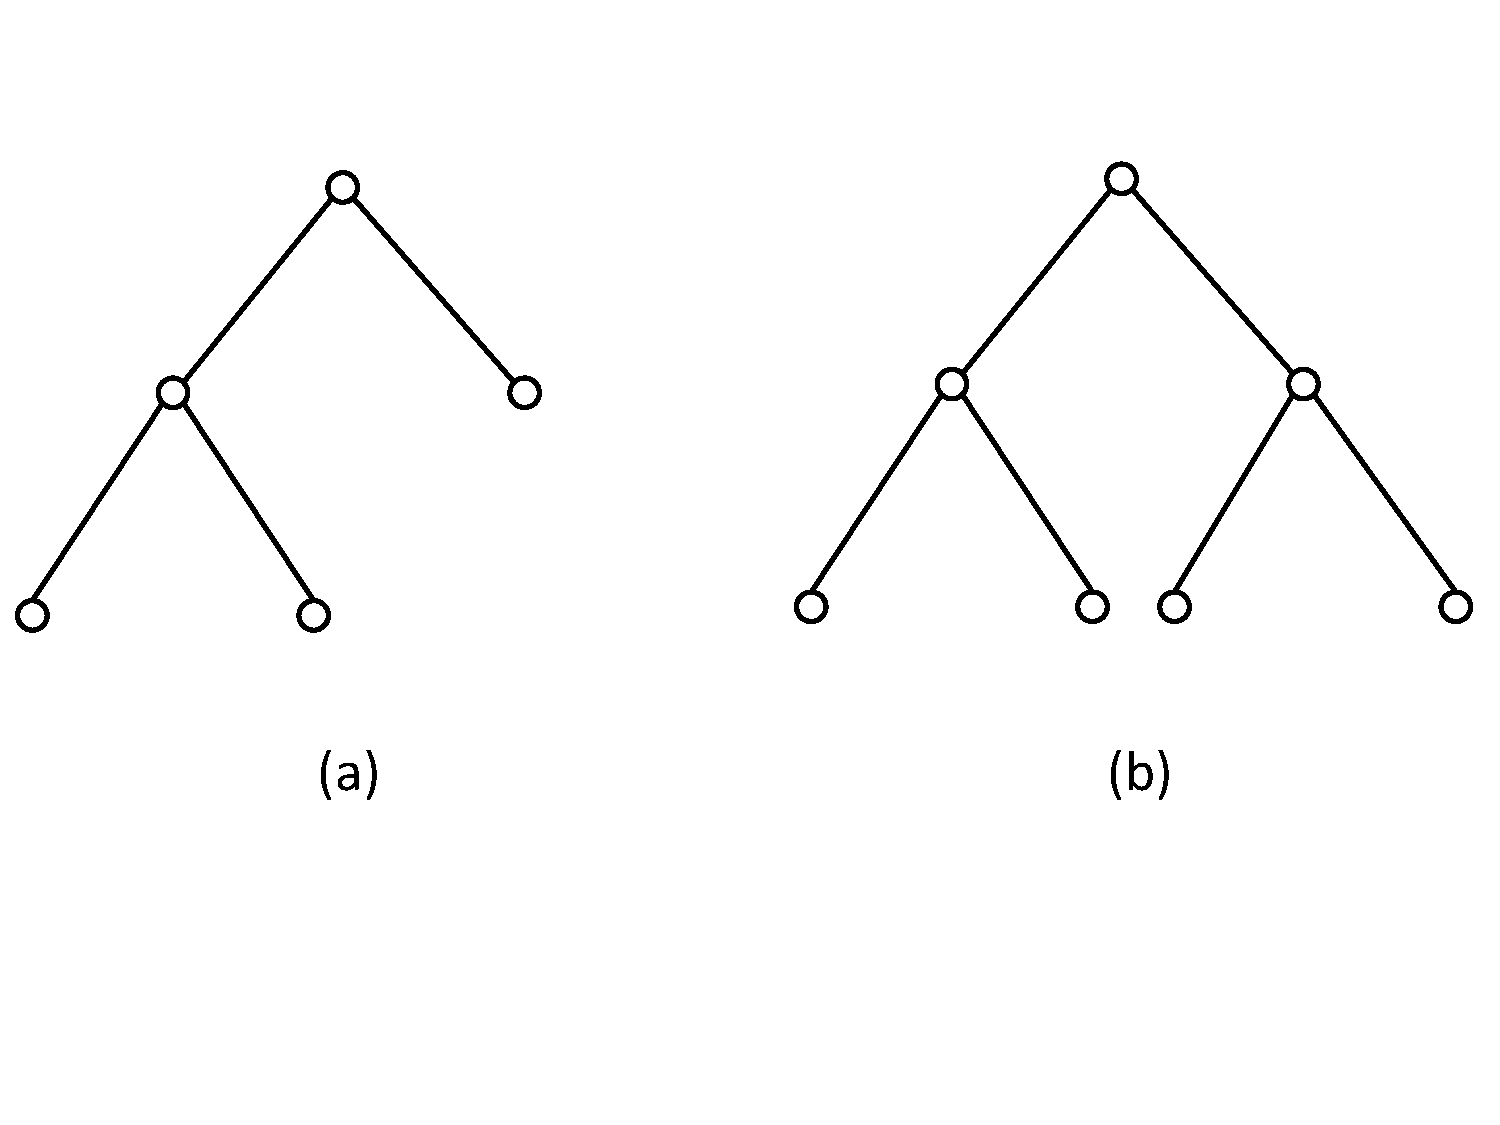
\includegraphics[scale=0.4]{../figures/fig2-4.pdf}
        \vspace{-50pt}
\caption{Example of $m$-ary trees}
\label{example of m-ary tree}
\end{figure}

\end{example}

As we mentioned in Chapter 1, this thesis will only deal with graph labelling problems with distance three constraint. For a complete $m$-ary tree $\tmk$ to be eligible for distance three labelling, we require the diameter of $\tmk$ to be no less than $3$. Thus, the height $k$ of $\tmk$ needs to be at least $2$, and the number of children $m$ of each vertex needs also to be at least $2$. In other words, all the complete $m$-ary trees $\tmk$ in this these have $k \ge 2$ and $m \ge 2$. Throughout the thesis we will now assume that these conditions are satisfied. 

The next remark shows how to construct a complete tree with height $k+1$ from complete $m$-ary tree with height $k$. 
 
\begin{remark}
\label{construct}
Take $m$ copies of a complete $m$-ary tree $\tmk$ and name the root of each single copy $u_0^i$, where $i \in [1,m]$. Connect each $u_0^i$ by an extra edge to the new vertex $u_0^0$. (Fig. \ref{example of construct}) The resulted graph is a complete $m$-ary tree with height $k+1$. The root of this larger complete $m$-ary tree $T_{m,k+1}$ is $u_0^0$. 

\begin{figure}
\centering
      \vspace{-0pt}
    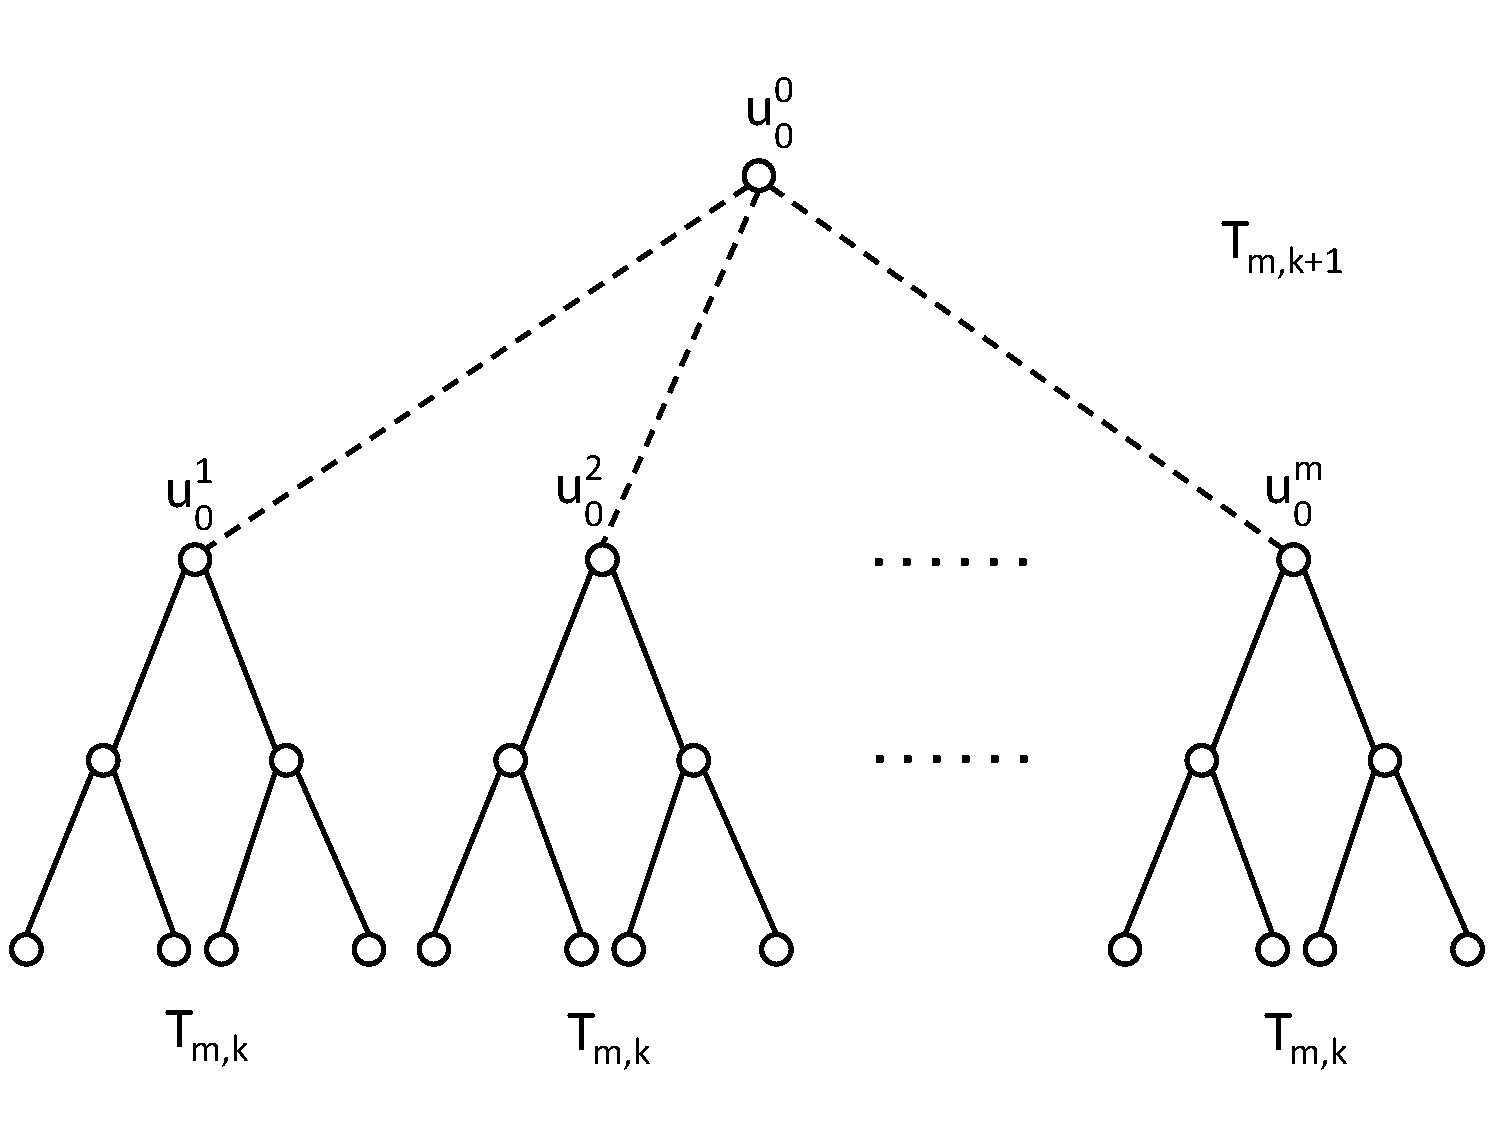
\includegraphics[scale=0.4]{../figures/fig2-5.pdf}
        \vspace{-0pt}
\caption{Construct $T_{m,k+1}$ from $\tmk$}
\label{example of construct}
\end{figure}
\end{remark}

Now, we have finished introducing most of the definitions that will be used throughout this thesis. It is time to start presenting our results.








\chapter{Linear metric labelling problem}

In this chapter, we will present one of the major results in this thesis, the $L(p_1,p_2,p_3)$-labelling of complete $m$-ray trees. Since there are only three parameters in this labelling system, from this time onwards we will call it $\lhpq$-labelling, unless we refer to a labelling system with infinitely many parameters. In the first section, we will give definitions and notation. We will then present a review of some know results. In Section 3.3, we present our results of $L(h,1,1)$-labelling of complete $m$-ary trees. Section 3.4 extend the $L(h,1,1)$-labelling result of complete $m$-ary trees to the general case; i.e., the $\lhpq$-labelling of complete $m$-ary trees. In the last section, we move onto the $\lhpq$-labelling of a broader class of trees that contain the set of complete $m$-ary trees as a subset. 



\section{Definitions and notation}

A linear metric $\lhpq$-labelling of a graph $G$ is an assignment of vertices of $G$ to non-negative integers such that vertices at distance $1$, $2$ or $3$ apart are mapped to integers with difference at least $h, p$ or $q$. Precisely, we have the following definition: 
\begin{definition}
A graph $G$ is said to be $\lhpq$-labelled if there is a map  
\[
f : V(G) \rightarrow \{0, 1, 2, \dots\}, 
\]
which respects the following constraints: 
\begin{itemize}
\item $|f(u) - f(v)| \ge h$, if $uv \in E(T)$;
\item $|f(u) -f(v)| \ge p$, if $d(u,v) = 2$;
\item $|f(u) - f(v)| \ge q$, if $d(u,v)=3$,
\end{itemize}
where $h\ge p \ge q \ge 1$ are integers. 
\end{definition}

According to this definition, it is noticed that there exists a maximum and a minimum label. Therefore, we define the \textit{span} of an $\lhpq$-labelling of a graph $G$ to be the difference between these maximum and minimum label for vertices of $G$. We use $span(f)$ to denote this concept. Furthermore, the {\it{minimum span}} of the labelling $f$ on the graph $G$ is defined as the smallest span over all $\lhpq$-labellings of $G$. The standard notation for the minimum span of an $\lhpq$-labelling of a graph $G$ is $\lamhpq(G)$.

\begin{remark}
\label{0}
Since the above function $f$ assigns non-negative integers to vertices of a graph $G$, it is convenient to always set the minimum label to be $0$. In this case, the span of $f$ is just the maximum label used by $f$, and the minimum span is the smallest maximum label assigned to vertices of $G$ by some $\lhpq$-labellings. 
\end{remark}

Let us go through an example of an $L(h,1,1)$-labelling of a complete $m$-ary tree. 

\begin{example}
Let $T_{2,2}$ be a complete $m$-ary tree with height $2$. Consider two different $L(2,1,1)$-labellings,  $f_1$ and $f_2$ on $T_{2,2}$ as shown in Fig. \ref{linear metric labelling} (a) and (b) respectively.

According to the above definitions, we have $span(f_1) = 7$ and $span(f_2) = 5$. In fact, it will be proved in Section 3.3 that the minimum span of $L(2,1,1)$-labelling of $T_{2,2}$ equals $span(f_2)$; i.e., $\lambda_{2,1,1}(T) = span(f_2) = 5$. 
  

\begin{figure}
\centering
      \vspace{-10pt}
    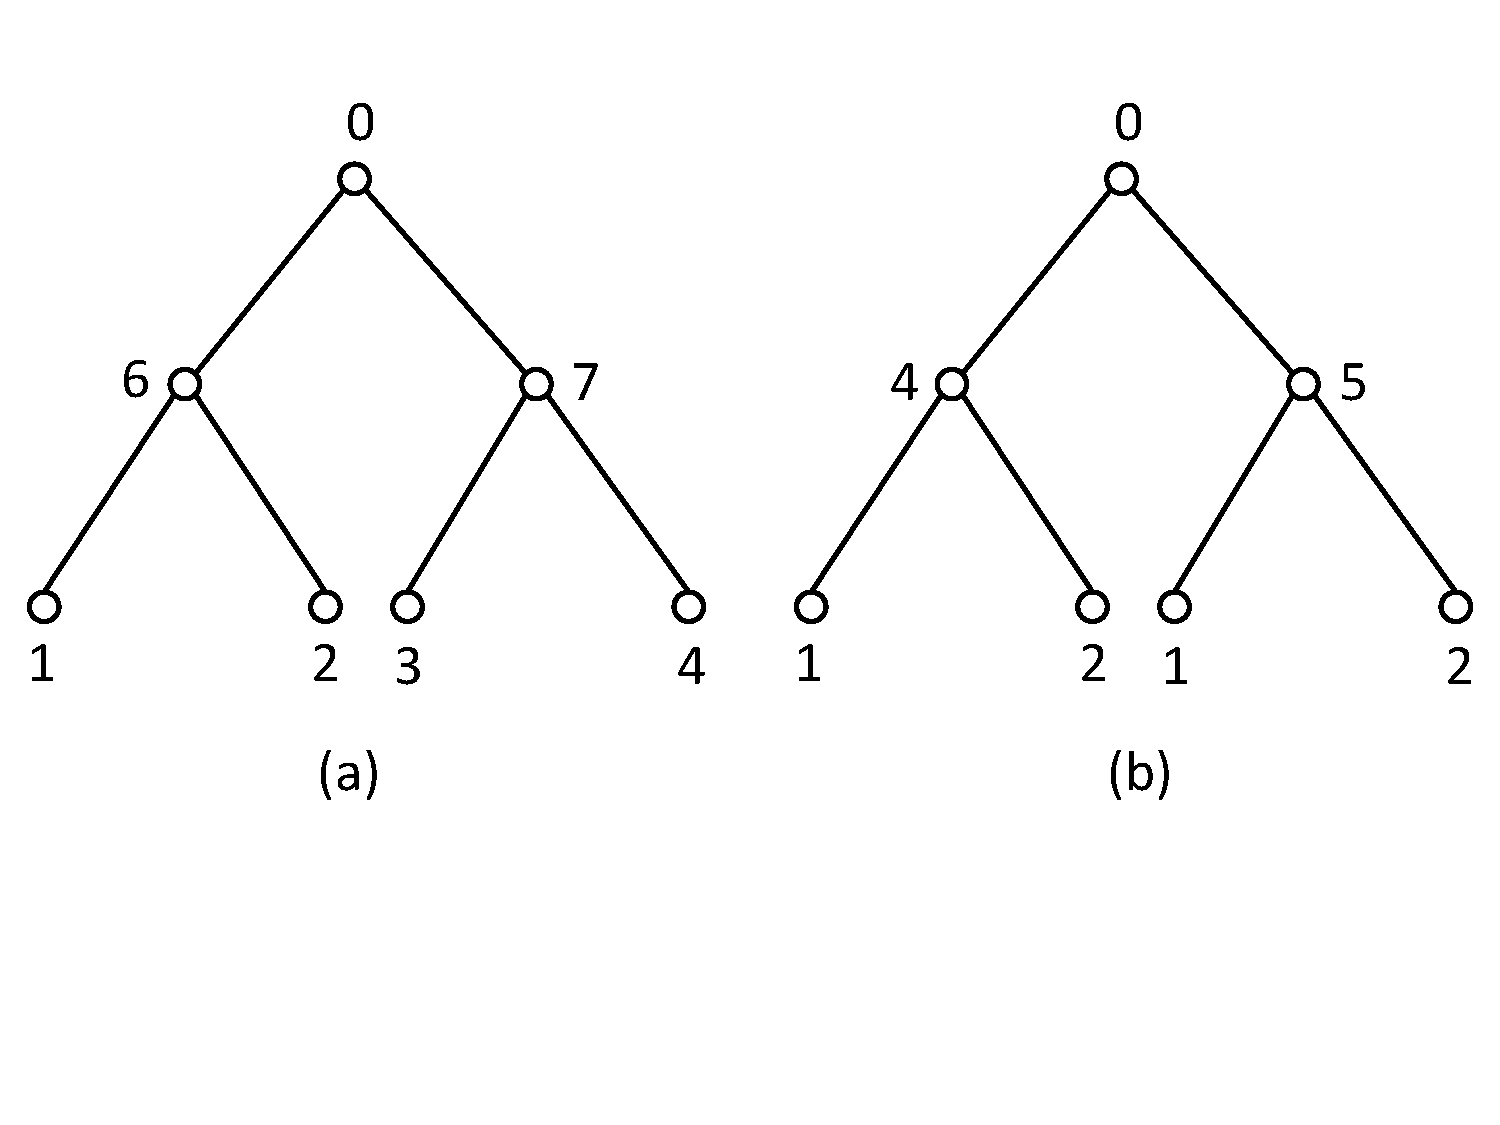
\includegraphics[scale=0.4]{../figures/fig3-1.pdf}
        \vspace{-50pt}
\caption{Two $L(h,1,1)$-labellings of $T_{2,2}$}
\label{linear metric labelling}
\end{figure}

\end{example}




%%%%%%%%%%%%%%%%%%%%%%%%%
\section{Known results for linear metric labelling problems}

In this section, we give the reader some ideas of what have been done in this area. It will include many linear metric labelling results for different types of graphs. Just remind the reader that we use $\Delta$ to denote the maximum degree of a graph. 

%For distance two constraints linear metric $L(p_1, p_2)$-labelling, when $p_1=p_2=1$ it is what we normally called graph clolouring. In this case, the minimum span is just the chromatic number for graph colouring. In the following, we will give some $L(1,1)$-labelling results of graphs. 

\subsection{Paths and cycles}

One of the earliest graph labelling problems is the $L(2,1)$-labelling of graphs, which was studied by \cite{yeh90} in his Ph.D thesis. Yeh first presented $L(2,1)$-labelling results of an $n$ vertices path $P_n$. He proved that the minimum span
\begin{align*}
\lambda_{2,1}(P_n) = 
\begin{cases}
2 & \text{ if } n = 2,\\
3 & \text{ if } n = 3 \text{ and }4,\\
4 & \text{ if } n \ge 5.
\end{cases}
\end{align*}
Based on this result, \cite{griggs92} proved that $\lambda_{2,1}(C_n) = 4$, for any $n$-cycle $C^n$. Later on, \cite{georges95} solved an even general problem. They proved that for $p_1 \ge p_2 \ge 1$, the minimum span of the $L(p_1, p_2)$-labelling of $P_n$ is 
\begin{align*}
\lambda_{p_1, p_2}(P_n) = 
\begin{cases}
0 & \text{ if } n =1, \\
p_1 & \text{ if } n = 2, \\
p_1 + p_2 & \text{ if } n = 3 \text{ or } 4, \\
p_1 + 2p_2 & \text{ if } n \ge 5 \text{ and } p_1 \ge 2p_2, \\
2p_1 & \text{ if } n \ge 5 \text{ and } p_1 \le 2p_2. 
\end{cases}
\end{align*}
If $p_1 \ge p_2 \ge 1$ and $p_1/p_2 > 2$, then the minimum span of the $L(p_1, p_2)$-labelling of $C^n$ is 
\begin{align*}
\lambda_{p_1, p_2}(C_n) = 
\begin{cases}
2p_1 & \text{ if } n \ge 3 \text{ is odd}, \\
p_1+2p_2 & \text{ if } n \equiv 0 \pmod{4}, \\
2p_1 & \text{ if } n \equiv 2 \pmod{4} \text{ and } p_1/p_2 \le 3,\\
p_1+3p_2 & \text{ if } n \equiv 2 \pmod{4} \text{ and } p_1/p_2 >3,
\end{cases}
\end{align*} 
If $p_1 \ge p_2 \ge 1$ and $p_1/p_2 \le 2$, then 
\begin{align*}
\lambda_{p_1, p_2}(C_n) = 
\begin{cases}
2p_1 & \text{ if } n \equiv 0 \pmod{3}, \\
4p_2 & \text{ if } n = 5, \\
p_1 + 2p_2 & \text{ otherwise.} 
\end{cases}
\end{align*}

%%%%%%%%%%%%%%%%%%%%%%%%%%%%%%%%%%%%%%%
\subsection{Trees}

\citet{griggs92} in the same paper also proved that the minimum span of the $L(2,1)$-labelling of any tree $T$ with maximum degree $\Delta \ge 1$ is $\Delta+1$ or $\Delta+2$. \cite{chang00} generalised Griggs and Yeh's studies to the $L(h,1)$-labelling problem and proved that the minimum span $\Delta+d-1 \le \lambda_{h, 1}(T) \le \min\{\Delta+2d-2, 2\Delta+d-2\}$, where both the lower and upper bounds are attainable. 

For distance three constraint linear metric labelling problem  of trees, there are also many well-known results. One of the most significant results proved by \cite{zhou10} is the $L(h,1,1)$-labelling problem for trees. The authors proved that the minimum span of the $L(h,1,1)$-labelling of any finite tree $T$ with diameter at least $3$ or an infinite tree with finite maximum degree is bounded as follows: 
\begin{align*}
&\max \left\{\max_{uv \in E(T)} \min \{d(u), d(v)\} +h-1, \Delta_2(T) -1\right\} \\
&\le \lambda_{h,1,1}(T) \le \Delta_2(T) +h-1 
\end{align*}
where $\Delta_2(T) := \max_{uv \in E(G)} (d(u) + d(v))$. Such an edge $uv \in E(T)$ is called an \emph{heavy edge}.  

Furthermore, define $\delta^*(T) := \min_{u \in V(T), d(u) \ge 2} d(u)$. \citeauthor{zhou10} proved that if $h \le \delta^*(T)$, then the upper bound can be decreased by $1$; i.e., $\lambda_{h,1,1}(T) \le \Delta_2(T) +h-2$. They also proved that for some special trees such as the caterpillar, both the lower bound and the improved upper bound are attainable. 


 
 
%%%%%%%%%%%%%%%%%%%%%%%%%%%%%%%%%%%%%%%%%%%%%%%%

\subsection{Planar graphs}
If a graph can be drawn on a plane without edge crossing, then we say such a graph is a \emph{planar graph}. 

For the $L(1,1)$-labelling of planar graphs, \cite{wegner97} conjectured
\begin{align*}
\lambda_{1,1}(G) = \chi(G) \le 
\begin{cases}
(3/2\Delta) + 1 & \text{ if } \Delta \ge 8, \\
\Delta+4 & \text{ if } 4 \le \Delta \le 7, \\
7 & \text{ if } \Delta = 3.
\end{cases} 
\end{align*}
Moreover, he conjectured that for $\Delta = 3$, the upper bound can be reduced to $6$. These two conjectures are still open for now. 

Recently, many people proved upper bounds for the chromatic number $\chi(G)$ of planar graphs $G$. Among all these results, the most impressive one is published by \cite{molloy05}. They proved that $\lambda_{1,1}(G) \le \lceil \frac{5}{3}\Delta \rceil + 77$ for any planar graph $G$. In particular, if $G$ has maximum degree $\Delta \ge 241$ then $\lambda_{1,1}(G) \le \lceil \frac{5}{3}\Delta \rceil + 24$. 

For $L(2,1)$-labelling of planar graphs $G$, \cite{jonas93} proved that $\lambda_{2,1}(G) \le 8\Delta - 13$. This bound was improved by \cite{van03} when solving the $L(p_1,p_2)$-labelling problem of planar graphs. They proved that the minimum span for any planar graph $G$ is bounded by $\lambda_{p_1,p_2}(G) \le (4p_2-2)\Delta + 10p_1+38p_2-23$, where $p_1 \ge p_2 > 0$. Later on, this upper bound is further improved to $p_2\lceil \frac{5}{3} \Delta \rceil + 18p_1+77p_2-18$ by \cite{molloy05}.

%%%%%%%%%%%%%%%%%%%%%%%%%%%%%%%%%%%%%%%%%%%%%%%%

\subsection{Outerplanar graphs} 
\label{linear outerplanar}
We say a graph is \emph{outerplanar} if drawing all its vertices on a path and its edges on one side of the path will not cause any edge crossing. Alternatively, an outerplanar graph is a graph such that when connecting an extra vertex to all its vertices does not cause any edge crossing. An outerplanar graph is planar, but the converse is not always true. 

\textbf{$L(1,1)$-labelling}. \cite{agnarsson04} proved an optimal upper bound for outerplanar graphs with smaller maximum degree $\Delta$. Precisely, for any outerplanar graph $G$, the minimum span is $\lambda_{1,1}(G) \le \Delta+2$ if $\Delta=2$ and $\lambda_{1,1}(G) \le \Delta+1$ if $\Delta=3,4$ and $6$. 
\\
\\
\textbf{$L(2,1)$-labelling.} \cite{jonas93} in his paper also proved an upper bound for the minimum span of the $L(2,1)$-labelling of outerplanar graphs $G$; i.e., $\lambda_{2,1}(G) \le 2\Delta+2$. Based on this result, \cite{bodlaender04} in their paper improved this upper bound to $\Delta+8$. More importantly, they conjectured that the bound can be improved to $\Delta+2$. Motivated by this, \cite{calamoneri04} proved the conjecture to be true for $\Delta \ge 8$ but false for $\Delta=3$. They also proved that $\lambda_{2,1}(G) \le \Delta+5$ for any outerplanar graph $G$ with $\Delta=3$. \cite{zhou11} recently improved \citeauthor{calamoneri04}'s upper bound to $\lambda_{2,1}(G) \le \Delta+3$ for every outerplanar graph $G$ with maximum degree $\Delta=3$. They mentioned in the paper that this bound is attainable by infinitely many outerplanar graphs. 
\\
\\
\textbf{$L(h,1,1)$-labelling.} For distance three constraint linear metric labelling of outerplanar graphs, \cite{calamoneri07} proved that $3\Delta-3 \le \lambda_{1,1,1}(G) \le  4\Delta-2$. In particular, the upper bound can be improved to $3\Delta+9$ if $G$ has maximum degree $\Delta \ge 6$. As a general result, they proved that $\lambda_{h,1,1}(G) \le 3\Delta+2h+7$ for $\Delta \ge h+5$. 

So far, we introduced to the readers many well-known results in this ares. In the following, we will present our own results. 



%%%%%%%%%%%%%%%%%%%%%%%%%%%%%%%%%%%%%%%%%%%%%%%%






%%%%%%%%%%%%%%%%%%%%%%%
\section{The $L(h,1,1)$-labelling of complete $m$-ary trees}
Let  $u_0 \in V(\tmk)$ be the root of $\tmk$, $u_i \in V(\tmk)$ be the vertex that is distance $1$ to $u_0$; $u_{ij} \in V(\tmk)$ be the vertex that is distance $2$ to $u_0$. In general, 
%First, let us define some new notations for complete $m$-ary trees that. Note that these notations are not standard, they are just for the convenience of proofs regarding to complete $m$-ary trees. We define the following: 
%\begin{itemize}
%\item $\VV_i := \{u \in V(\tmk) \mid d(u, u_0) = i\}$, where $i \in [1,m]$
%\item $C(u) :=$ children of a vertex $u \in V(\tmk)$
%\item $P(u) :=$ parent of a vertex $u \in V(\tmk)$
$u_{\underbrace{ij\dots k}_\text{n}} \in V(\tmk)$ is the vertex that is distance $n$ to the root $u_0$, for $i, j, \dots, k \in [1, m]$. \footnote{Define $[1,m]:=\{1, 2, 3, \dots, m-1, m\}$.} 
%\end{itemize}


\begin{lemma}
\label{reuse}
Suppose $f$ is an $L(h,1,1)$-labelling of a complete $m$-ary tree $\tm2$. Then it is possible to assign same labels to $C(u_i)$ and $C(u_j)$ for $i \neq j$ without causing conflict,\footnote{By causing conflict we mean the map $f$ violates the $L(h,1,1)$-labelling conditions.} that is, 
\[
f(C(u_i)) = f(C(u_j)), \text{ for } i \neq j. 
\]
\end{lemma}

\begin{proof}
Without loss of generality, let us consider the sets $C(u_1)$ and $C(u_2)$. We know that $u_{1j} \in C(u_1)$ and $u_{2j} \in C(u_2)$, then for all $j \in [1,m]$ it follows that 
\begin{align}
\label{dis4}
d(u_{1j}, u_{2j}) = 4.
\end{align}
By conditions of $L(h,1,1)$-labelling, $u_{1j}$ and $u_{2j}$ can receive the same label. Thus in general, $C(u_i)$ and $C(u_j)$ can be labelled by the same labels.  
\end{proof}
\qed

\begin{lemma}
\label{lem:consh11} Let $f$ be an $L(h,1,1)$-labelling of a complete $m$-ary tree $\tm2$. Suppose $f$ labels $\tm2$ in the following way: 
\begin{enumerate}[(1)]
\item $f(N(u_1))$ and $f(C(u_0))$ are consecutive label sets for vertices of $\tm2$;
\item $\min \{f(N(u_1))\} - \max\{f(C(u_0))\} = h$ or $\min\{f(C(u_0))\} - \max\{f(N(u_1))\} = h$.
\end{enumerate}
Then, for any other $L(h,1,1)$-labelling of $\tm2$, say $g$, we have 
\begin{align}
\label{minimum}
span(f) \le span(g). 
\end{align}
More importantly, the span of $f$ achieves an exact value, that is, 
\begin{align}
\label{exact} 
span(f)= 2m+h-1. 
\end{align}
\end{lemma}

Note that according to Lemma \ref{reuse}, here we only deal with $f(N(u_1))$ as $f(C(u_i)) = f(C(u_j))$ for $i \neq j$.
\\
\begin{proof}
The proof of this lemma refers to the proof of Lemma \ref{lem:conshpq}, which is a generalised version of this lemma. 
\end{proof}
\qed
\\
%As a bound for the minimum span of $L(h,1,1)$-labelling on trees is given by Theorem \ref{thm:deb} (Refer to Theorem $1$ in {deborah}), we can start with applying this theorem to the family of complete $m$-ary trees. If possible, improve the bound from then. 

%Notice that for a complete $m$-ary tree $T$, the $\Delta_2$ value varies for different height of $T$. In particular, $\Delta_2(T) = 2m+1$ for height $k=2$ and $\Delta_2(T) = 2m+2$ for height $k \ge 3$. By Theorem \ref{thm:deb}, we have 

%\begin{align*}
%\max\{m+h-1, 2m\} &\le \l \le 2m+h, \text{ when } k = 2 \\
%\max\{m+h, 2m+1\} &\le \l \le 2m+h+1, \text{ when } k \ge 3
%\end{align*}

%By definition of $\delta^*(T)$ \cite{zhou00}, for a complete $m$-ary trees $T$ we have $\delta^*(T) = m$. Assume $h \le m =  \d$, we have $2m > m+h-1$ and $2m+1 > m+h$. By improvement of the upper bound in \cite{zhou00}, the upper bounds above can also be improved. Thus we have 

%\begin{align}
%2m &\le \lambda_{h,1,1}(T) \le 2m+h-1, \text{ when } k = 2 \text{ and } h \le m \\
%\label{kge3hlem}
%2m+1 &\le \lambda_{h,1,1}(T) \le 2m+h, \text{ when } k \ge 3 \text{ and } h \le m
%\end{align}

%Assume $h > m$, then results in \cite{zhou00} do not reduce the upper bound. Hence we have 
%\begin{align}
%m+h-1 &\le \l \le 2m+h, \text{ when } k = 2 \text{ and }h > m \\
%\label{kge3hgm}
%m+h &\le \l \le 2m+h+1, \text{ when } k \ge 3 \text{ and } h > m
%\end{align}
The following is our major result for the minimum span of $L(h,1,1)$-labelling problems on the family of complete $m$-ary trees. 

\begin{theorem}
\label{thm:h11} 
For a complete $m$-ary tree $\tmk$, the minimum span of $L(h,1,1)$-labelling of $\tmk$ is
\begin{align}
\label{h11}
 \lambda_{h,1,1}(\tmk) =
  \begin{cases}
   2m+h-1 & \text{for } k = 2, \\
   2m+h       & \text{for } k \ge 3.
  \end{cases}
\end{align}
\end{theorem}

To prove this theorem, let us see the following lemma first. 
\begin{lemma}
\label{subtree} 
Let $T_{n,l}$ be a complete $n$-ary tree with height $l$, where $n \le m$ and $l \le k$. Then $\tmk$ contains $T_{n,l}$ as a subtree. We claim that 
\[
\lambda_{h,1,1}(T_{n,l}) \le \lambda_{h,1,1}(\tmk).
\] 
\end{lemma}

\begin{proof}
The proof is straightforward. If $\lamh11(T_{n,l}) > \lamh11(\tmk)$, then it contradicts the assumption that $\lamh11(\tmk)$ is the minimum span of $L(h,1,1)$-labelling of $\tmk$. 
\end{proof}
\qed

The general version of this lemma is also true. That is, for any tree $T$ and its subtree $T' \subseteq T$, we have $\lamh11(T') \le \lamh11(T)$. 

 We will give a detailed proof of Theorem \ref{thm:h11} in the following. As this is the first formal proof in  this thesis, we will spend some time to explain the structure of the proof as it is similar to other proofs in the thesis. 

To prove that the minimum span $\lamh11(\tmk)$ achieves particular value, we first show that this value is the lower bound of $\lamh11(\tmk)$. Normally we prove this by contradiction. Then we need to show that there exits a map $f$ that $L(h,1,1)$-labels $\tmk$ with $span(f)$ equal to that value. This step sometimes is the hardest part, because it is not easy to construct or find a labelling system for infinite graphs. Another option for proving this step is to use induction. 
\\
\begin{proof}{\bf of Theorem \ref{thm:h11}}
First, we want to prove the minimum span $\lamh11(\tm2) \ge 2m+h-1$. As we proved in Lemma \ref{reuse} that labels can be re-used by sets $C(u_i)$ and $C(u_j)$ for different $i$ and $j$, then when $L(h,1,1)$-labelling a complete $m$-ary tree $\tm2$, it is sufficient to consider the minimum useful subtree \footnote{Minimum useful subtree here means the  minimum subtree of $\tm2$ that achieves the same $\lambda_{h,1,1}$ value as $\tm2$.} as shown in Fig. \ref{useful part}. 

\begin{figure}
\centering
      \vspace{-10pt}
    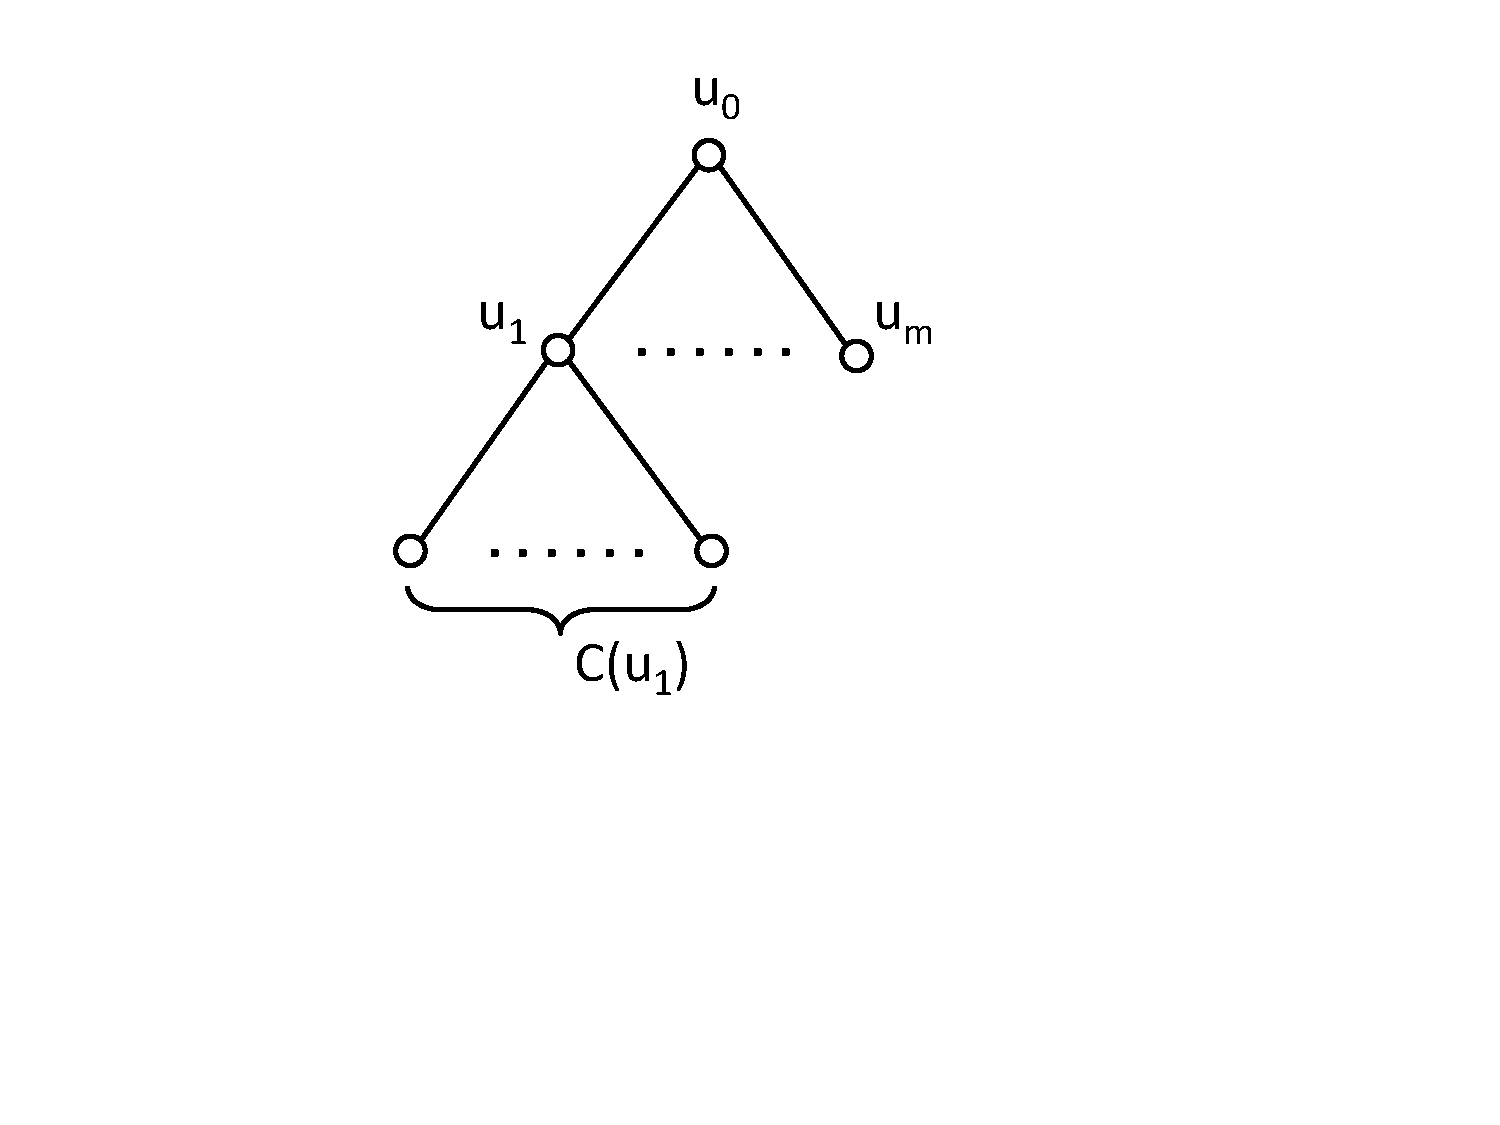
\includegraphics[scale=0.4]{../figures/fig3-2.pdf}
        \vspace{-80pt}
\caption{Minimum useful subtree of $T_{m,2}$}
\label{useful part}
\end{figure}

Now, assume the minimum span is $\lamh11(\tm2) \le 2m+h-2$. The minimum subtree contains $2m+1$ vertices that are within distance three to each other, so we need at least $2m+1$ labels to label it. More importantly, we need to have a gap with size at least $h$ between the two label sets $f(N(u_1))$ and $f(C(u_0))$. Thus in total, we need $2m+h-1$ labels to $L(h,1,1)$-label the minimum subtree of $\tm2$. This contradicts the assumption that $\lamh11(\tm2) \le 2m+h-2$. 

Lemma \ref{lem:consh11} shows that for $k = 2$, we can find an $L(h,1,1)$-labelling $f$ of $\tm2$ with $span(f) \le 2m+h-1$. Thus we are done for the minimum span of complete $m$-ary trees $\tm2$. 

By Remark \ref{construct}, we can build a complete $m$-ary tree $T_{m,k+1}$ from a complete $m$-ary tree $\tmk$. In particular, we can build $T_{m,3}$ from $\tm2$. We proved that $\lamh11(\tm2) = 2m+h-1$. Hence the minimum span $\lamh11(T_{m,3})$ is at least $2m+h-1$. However, the new vertex that is brought in when building up $T_{m,3}$ is within distance three to every other vertices in $T_{m,3}$, we must add an extra label to the original label set for $\tm2$. Thus we have $\lamh11(T_{m,3}) \ge 2m+h$. In general, we have $\lamh11(\tmk) \ge 2m+h$ for $k \ge 3$. 

It  remains to show that $\lambda_{h,1,1}(\tmk) \le 2m+h$ for $k \ge 3$. To prove this we need to find a function $f$ that $L(h,1,1)$-labels $\tmk$ such that $span(f) = 2m+h$. Though we are dealing with infinite complete $m$-ary trees, it seems when labelling these trees, there is a patten that can be followed. The idea is to pre-define two label sets. We assign one of these two label sets to each level of $\tmk$ alternatively. Precisely, we let $S_1:=[0,m], S_2:= [m+h, 2m+h]$ be two integer sets. Then the function $f$ labels $\tmk$ as follows (Fig. \ref{lh11}): 
\begin{enumerate}[(1)]
\item $f(u_0) = 0$;
\item $\{f(u_{i}) \mid i \in [1,m]\} = \SS_2 \setminus \{2m+h\}$ such that $f(u_{i}) = m+h+i-1$;
\item 
$
 f(C(u_{0\dots ijk})) =
  \begin{cases}
   \SS_1 \setminus f(P(u_{0\dots ijk})) & \text{if } d(u_0, u_{0\dots ijk}) \text{ is odd}, \\
   \SS_2 \setminus f(P(u_{0\dots ijk})) & \text{if } d(u_0, u_{0\dots ijk}) \text{ is even}. 
  \end{cases}$
\end{enumerate}

\begin{figure}
\centering
      \vspace{-10pt}
    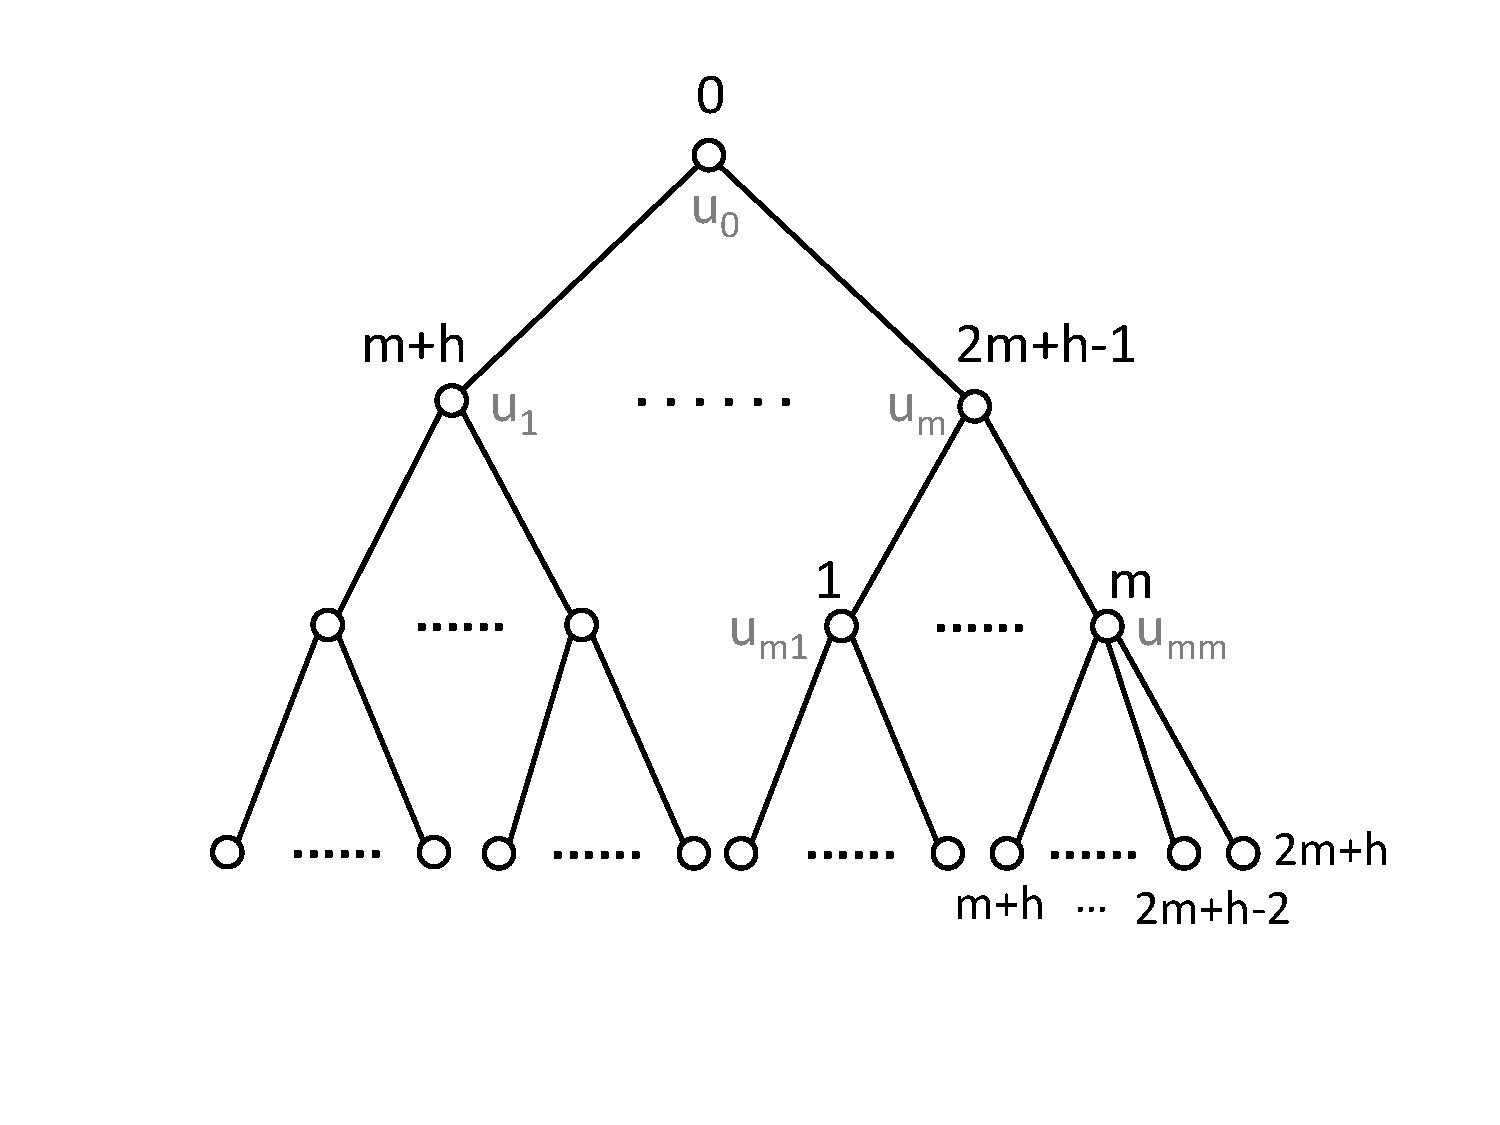
\includegraphics[scale=0.4]{../figures/fig3-3.pdf}
        \vspace{-30pt}
\caption{The $L(h,1,1)$-labelling of $T_{m,3}$ with span equals $2m+h$}
\label{lh11}
\end{figure}

It is not hard to see that $f$ perfectly $L(h,1,1)$-labels $\tmk$ with $span(f) = 2m+h$. This completes the proof of this theorem. 
\end{proof}
\qed

\begin{corollary}
\label{thm:111} For a complete $m$-ary tree $\tmk$, the minimum span of $L(1,1,1)$-labelling is 
\begin{align*}
 \lambda_{1,1,1}(\tmk) =
  \begin{cases}
   2m & \text{for } k = 2, \\
   2m+1       & \text{for } k \ge 3.
  \end{cases}
\end{align*}
\end{corollary}

This corollary agrees with Corollary $5$ in the paper published by \cite{zhou10}. They claimed that for a finite tree $T$ with diameter at least $3$ or an infinite tree with finite maximum degree, the following holds: 
\[
\chi(T^3) = \lambda_{1,1,1}(T) + 1 = \Delta_2(T).
\] 

\begin{remark}
For every tree $T$, there exits a complete $m$-ary tree $\tmk$ such that $T \subseteq \tmk$ is a subtree. Thus by the generalisation of Lemma \ref{subtree}, we have $\lamh11(T) \le \lamh11(\tmk)$ where $T \subseteq \tmk$ is a subtree. As we proved $\lamh11(\tmk)$ to be exact values, it follows that these values can be used as the upper bound for $\lamh11(T)$. Then we have the following: 
\begin{align*}
\lamh11(T) \le 
\begin{cases}
2m+h-1 & \text{ for } k =2, \\
2m+h & \text{ for } k \ge 3.
\end{cases}
\end{align*}
where $T$ is a finite tree or an infinite tree with finite maximum degree such that $diam(T) \ge 3$, and $k$ is the height of the minimal \footnote{In this case, we say the complete $m$-ary tree is minimal if it is contained in all other complete $m$-ary trees, in which $T$ is a subtree.} complete $m$-ary tree $\tmk$ that contains $T$ as a subtree. 
\end{remark} 

So far we have presented our first major theorem in this thesis. Based on this theorem, we slightly improved the upper bound stated by Theorem $1$ in \cite{zhou10}. In the next section, we will extend the $L(h,1,1)$-labelling problem to a more general and interesting version, the $\lhpq$-labelling problems.


%%%%%%%%%%%%%%%%%%%%%%%%%%%%%%%%%%%

\section{The $L(h,p,q)$-labelling of complete $m$-ary trees}

Previously, we studied the $L(h,1,1)$-labelling of complete $m$-ary trees. We found an exact value for the minimum span $\lambda_{h,1,1}(\tmk)$ of a complete $m$-ary tree $T_{m,k}$, which depends on the parameters $m$ and $h$. Surprisingly, this value is independent of the tree height apart from the fact that the value for $k = 2$ is different from that for $k \ge 3$. 

Without restricting $p$ and $q$ to be $1$, it is reasonable to believe that the $\lambda_{h,p,q}$ values of $T_{m,k}$ can also be precisely determined, though  they may have dependence upon $p$ and $q$. Notice that the only restriction we demand is $h \ge p \ge q \ge 1$.

We promised in the previous section that we will prove Lemma \ref{lem:consh11}. In the following, we will state a similar but more general lemma than Lemma \ref{lem:consh11}. The proof of Lemma \ref{lem:consh11} is a special case of the following proof, in the case $p =q=1$. 

%To make life easier, we define the following notations.
%\begin{itemize}
%\item $\AA_{1} := \{\varphi(u_{0}), \varphi(C_{u_i}) \mid \forall i \in [1,m]\}$
%\item $\AA_1' := \{\varphi(C_{u_i}) \mid \forall i \in [1,m]\}$
%\item $\AA_{2} := \{\varphi(u_{i}) \mid \forall i \in [1,m]\}$
%\item $\CC_{1} := \{\phi(u_{0}), \phi(C_{u_i}) \mid \forall i \in [1,m]\}$
%\item $\CC_{2} := \{\phi(u_{i}) \mid \forall i \in [1,m]\}$
%\end{itemize}

%We call $\AA_1, \AA_2, \CC_1, \CC_2$ {\color{red} label sets} for vertices of $T$. Now, let us begin the following lemma. 

\begin{lemma}
\label{lem:conshpq} Suppose $f$ is an $\lhpq$-labelling of a complete $m$-ary tree $\tm2$ such that the following are satisfied: 

\begin{enumerate}[(1)]
\item $f(N(u_1))$ and $f(C(u_0))$ are $p$-consecutive label sets;\footnote{$f(N(u_1)) = \alpha_1 + pI_1$ and $f(C(u_0)) = \alpha_2 + pI_2$, where $I_1, I_2$ are integer sets. In particular, when $p = 1$, a $1$-consecutive set is just a consecutive set.} 
\item $\min (\lnu) - \max(\lcu) = h$ or $\min(\lcu) - \max(\lnu) = h$. 
\end{enumerate}
Then, for any other $\lhpq$-labelling of $\tm2$, say $g$, we have 
\begin{align}
\label{minimumhpq}
span(f) \le span(g). 
\end{align}
More importantly, $span(f)$ can be found exactly and is
\begin{align}
\label{exacthpq} 
span(f)= (2m-1)p+h. 
\end{align}
\end{lemma}

As in Lemma \ref{lem:consh11}, here we only deal with $f(N(u_1))$. The following is a formal proof of this lemma. 
\\
\begin{proof}
First, let us prove \eqref{exacthpq}. Without loss of generality, assign $\{0\}$ to the root $u_0$ of $\tmk$. Then we have $\{0\} \in \lnu$. We know that $|N(u_1)| = m+1$ and $|C(u_0)| = m$, then condition (1) and (2) imply $\lnu = [0,m]p$ and $\lcu = mp+h+[0,m-1]p$. Hence, the span of the function $f$ equals the maximum label used equals $(2m-1)p+h$. 

To prove \eqref{minimumhpq}, we need to study the function $g$ that satisfies various conditions. The easiest case is when $g$ satisfies both $(1)$ and $(2)$. Then \eqref{minimumhpq} holds, as $span(f) = span(g)$. 

It remains to check that \eqref{minimumhpq} always holds even if $g$ fails to obey at least one of the above two conditions. Without loss of generality, we assume $0 \in g(N_{u_1})$ for all the following cases. 
\\
\textbf{Case $1$.} The labelling $g$ satisfies condition $(1)$ but not $(2)$. 

(1) implies $\gnu= [0, m]p$. Since condition $(2)$ is not satisfied by $g$, we have $\min\{\gcu\} - \max\{\gnu\} \ge h+1$. By consecutiveness of $\gcu$, we have $\gcu = a+[0,m-1]p$, where $a \ge mp+h+1$. Thus, 
\begin{align*}
span(g) &= a+(m-1)p \\
&\ge (2m-1)p+h+1 \\
&> (2m-1)p+h\\
&= span(f).
\end{align*}
\textbf{Case $2.1$.} The labelling $g$ does not satisfy conditions $(1)$ and \\$[0, \max\{\gnu\}] \cap \gcu = \emptyset$. 

As condition $(1)$ is not satisfied, we have at least one of $\gnu$ and $\gcu$ is not consecutive. Without loss of generality, let us assume $\gnu$ is not consecutive. In this case, we have $\gnu \subsetneq [0, \max\{\gnu\}]$. From Case 1, we know that if $\gnu$ is consecutive, then $\gnu = [0,m]p$, so here we must have $\max\{\gnu\} > mp$ if $\gnu$ is not consecutive. Since it is not sure whether condition $(2)$ is satisfied, then for $g$ to $\lhpq$-label $\tm2$, we have 
$$\min\{\gcu\} -\max\{\gnu\} \ge h$$ 
provided $[0, \max\{\gnu\}] \cap \gcu = \emptyset$. Moreover, as the consecutiveness of $\gcu$ is unknown, we have
$$\gcu \subseteq [\min\{\gcu\}, \max\{\gcu\}],$$ 
where 
\begin{align*}
&\min\{\gcu\} \ge \max\{\gnu\}+h 
\intertext{and}
&\max\{\gcu\} \ge \min\{\gcu\}+(m-1)p. 
\end{align*}
Hence we have 
\begin{align*}
span(g) &= \max\{\gcu\} \\
&\ge \min\{\gcu\}+(m-1)p \\
&\ge \max\{\gnu\}+h+(m-1)p \\
&> mp+h+(m-1)p \\
&= (2m-1)p+h \\
&= span(f).
\end{align*}
\textbf{Case $2.2$.} The labelling $g$ does not satisfy condition $(1)$ and\\ $[0, \max\{\gnu\}] \cap \gcu \neq \emptyset$. 

First, let  
$I :=  [0, \max\{\gnu\}] \cap \gcu$ be the intersected part. By condition of Case 2.2, we have $|I| \neq 0$. 

%The map $g$ is an $\lhpq$-labelling of $\tm2$ ensures that $\gnu \cap \gcu = \emptyset$. Then we have $I \subsetneq \gcu$ is a proper subset. 

The violation of condition (1) implies at least one of $\gnu$ and $\gcu$ is not consecutive. Also, as $d(u,v) = 1$ for any vertices $u \in \gnu, v \in \gcu$, then $\gnu \cap \gcu = \emptyset$. We have assumed that $\{0\} \in \gnu$, then it is not possible for $\gnu$ to be consecutive, for otherwise $|I| = 0$. It is obvious that the more pieces $\gnu$ or $\gcu$ has, the larger $span(g)$ will be. Therefore, the smallest span is achieved in the case where $\gnu$ consists of two pieces and $\gcu$ is consecutive; i.e., $\gcu \subsetneq [0, \max\{\gnu\}]$. If we can prove that $span(g)$ obtained in this case is still no less than $span(f)$, then \eqref{minimum} is true. 
Let 
\begin{align*}
&\gnu = \gnu^1 \cup \gnu^2\\
\intertext{and} 
&S = [0, \max\{\gnu\}],
\end{align*}
where $\gnu^1$ and $\gnu^2$ are both consecutive label sets. 

Since $g$ is an $L(h,1,1)$-labelling of $\tm2$ and condition (2) is unknown, there exits two forbidden gaps\footnote{The part of labels that cannot be used when $L(h,1,1)$-label $\tm2$ is said to be forbidden gaps.} $\GG_1, \GG_2$ in between the sets $\gnu^1, \gcu$ and $\gcu, \gnu^2$ with cardinalities $|\GG_1| \ge h-1$ and $|\GG_2| \ge h-1$. Thus we have (Fig. \ref{case2.2})
\begin{align*}
S &= \gnu^1 \cup \GG_1 \cup \gcu \cup \GG_2 \cup \gnu^2. 
\end{align*}
This implies 
\begin{align*}
\max\{\gnu\}
&\ge (2m-2)p+2h.
\end{align*}
Note that $((2m-2)p+2h) - ((2m-1)p+h) = h-p \ge 0$, as $h \ge p$. Then we have $span(g) \ge span(f)$. This completes the proof of this lemma. 
\begin{figure}
\centering
      \vspace{-5pt}
    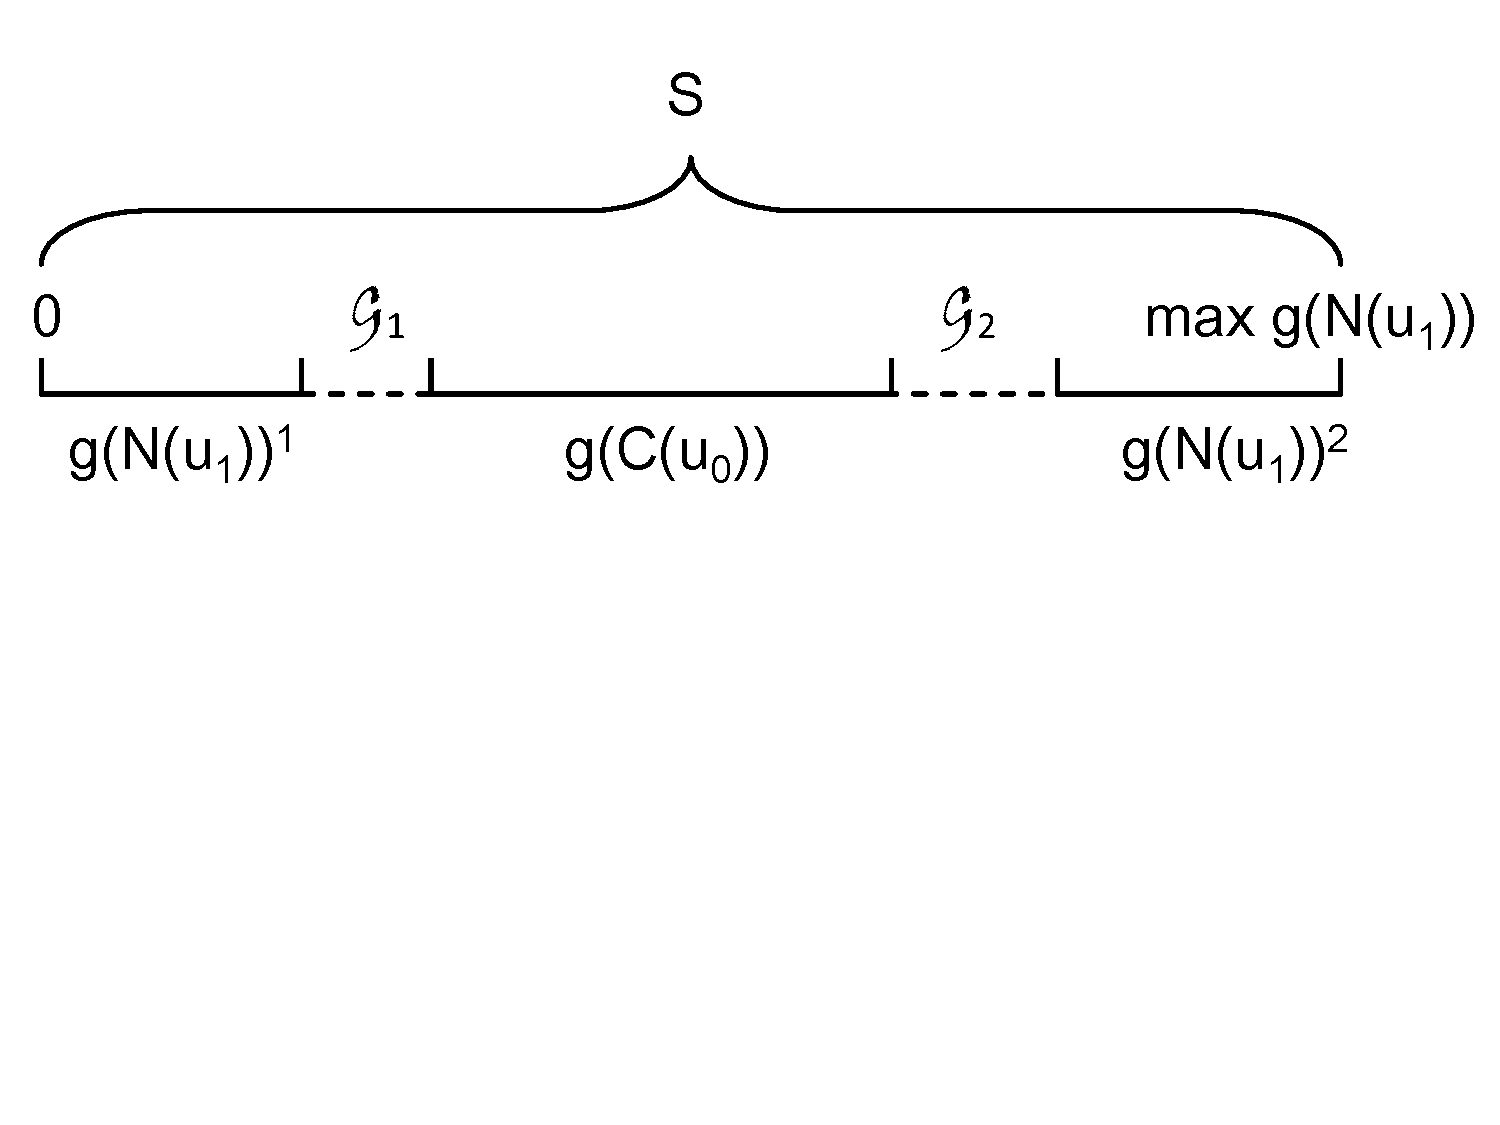
\includegraphics[scale=0.4]{../figures/fig3-4.pdf}
        \vspace{-110pt}
\caption{$\gcu \subsetneq [0, \max\{\gnu\}]$}
\label{case2.2}
\end{figure}
\end{proof}
\qed


\begin{remark}
\label{hpqtm2}
For any $L(h,p,q)$-labelling of a complete $m$-ary tree $\tm2$ under the conditions in Lemma \ref{lem:conshpq}, \eqref{minimumhpq} is always true. This implies the minimum span $\lamhpq(\tm2) \le span(f) = (2m-1)p+h$. On the other hand, it is not hard to see that to $\lhpq$-label $\tm2$, the minimum required label set is $[0, 2m-1]p+h$, so $\lambda_{h,p,q}(\tm2) \ge (2m-1)p+h$. Hence we have  
\begin{align}
\label{minispanhpq}
\lambda_{h,p,q}(T) = (2m-1)p+h.
\end{align}

\end{remark}


\begin{theorem}
\label{thm:hpq}
Let $h \ge p \ge q \ge 1$. For a complete $m$-ary tree $\tmk$, the minimum span of the $\lhpq$-labeling is
\begin{align}
\label{eq:thmhpq}
\lambda_{h,p,q}(\tmk) = 
 \begin{cases}
 (2m-1)p+h & \text{ when } k = 2, \\
 2mp+h & \text{ when } k \ge 3.
 \end{cases}
\end{align}
\end{theorem}

Substitute $p=q=1$ into \eqref{eq:thmhpq}, we get the same result as Theorem \ref{thm:h11}, that is, the minimum span of the $L(h,1,1)$-labelling of complete $m$-ary trees $\tmk$ is
\begin{align*}
 \lambda_{h,1,1}(\tmk) =
  \begin{cases}
   2m+h-1 & \text{for } k = 2, \\
   2m+h       & \text{for } k \ge 3.
  \end{cases}
 \end{align*}
In other words, Theorem \ref{thm:h11} is a special case of Theorem \ref{thm:hpq}. The proof of this theorem is similar to the proof of Theorem \ref{thm:h11}. We will first prove \eqref{eq:thmhpq} is a lower bound. Then we will construct specific $\lhpq$-labelling for $\tmk$ with span equals \eqref{eq:thmhpq}.  

Notice that this theorem claimed that the $\lamhpq$ value is independent of the third parameter $q$. This is due to the restriction $h \ge p \ge q \ge 1$. 
\\
\begin{proof}
Remark \ref{hpqtm2} proved that $\lamhpq(\tm2) = (2m-1)p+h$. Now, we want to show that $\lamhpq(\tmk) \ge 2mp+h$ for $k \ge 3$. 

We mentioned before that a complete $m$-ary tree $T_{m, 3}$ can be constructed from $\tm2$ by connecting one extra vertex to roots $\{u_0^1, \dots, u_0^m\}$ of $m$ copies of $\tm2$. During this construction, we introduced a new vertex $u_0$, which is within distance $3$ to every vertex in $m$ copies of $\tm2$. Then the minimum span $\lamhpq(T_{m,3}) \ge \lamhpq(\tm2) + p$. Thus we have $\lamhpq(\tmk) \ge \lamhpq(T_{m,3}) \ge 2mp+h$ for $k \ge 3$. 

It is remaining to show that \eqref{eq:thmhpq} is also the upper bound of $\lamhpq(\tmk)$ for $k \ge 3$. To prove this, we will construct similar labelling system as those before for $L(h,1,1)$-labelling of $\tmk$. 

Define $\SS_1: = [0,m]p$ and $\SS_2 := (mp+h)+[0,m]p$ to be the label sets we need. Below we provide details of how to $\lhpq$-label $\tmk$ for $k \ge 3$. 
\begin{enumerate}[(1)]
\item $f(u_0) = 0$;
\item $\{f(u_i) \mid i \in [1,m]\} = \SS_2 \setminus \{2mp+h\}$ such that $f(u_i) =(m+i-1)p+h$;
\item $f(C(u_{0 \dots ijk})) =
 \begin{cases}
 \SS_1 \setminus f(P(u_{0 \dots ijk})) & \text{ if } d(u_0, u_{0\dots ijk}) \text{ is odd, } \\
 \SS_2 \setminus f(P(u_{0 \dots ijk})) & \text{ if } d(u_0, u_{0\dots ijk}) \text{ is even.} 
 \end{cases}$
\end{enumerate}

Clearly $f$ is an $\lhpq$-labelling of $\tmk$ with $span(f) = 2mp+h$. This completes the proof of Theorem \ref{thm:hpq}. 
\end{proof}
\qed




%%%%%%%%%%%%%%%%%%%%%%%%%%%%%%%%%%%

\section{The $L(h,p,q)$-labelling of broader sets of trees}

From now on, we will generalise our $\lambda_{h,p,q}$ results to a more general set of trees, which contains the set of complete $m$-ary trees as a proper subset. 

We recall some notation defined earlier. We use $\Delta(T)$ (or $\Delta$) to denote the maximum degree of a tree $T$, the term $\Delta_2(T)$ (or $\Delta_2$) to denote the sum of the degrees of an heavy edge; $\Delta_2(T) := \max_{uv \in E(T)}((d(u) + d(v))$.
%%%%%%%%%%%%%%%%%%%%%%%%%%%%%%%%%%%




\subsection{The sets of trees with $\Delta_2$ value equals $2\Delta-1$ or $2\Delta$}
\label{sec:general sets}

To start, let us define the following: 
\begin{itemize}
\item Let $\TT := \{\tmk \mid m \ge 2, k\ge 2\}$ be the set of complete $m$-ary trees with $m, k \ge 2$.
\item Let $\TT^{(n)} := \{\tmk \in \TT \mid k=n\}$ be the set of complete $m$-ary trees with height exactly $n$. 
\item Let $\TT^{(\ge n)} := \{\tmk \in \TT \mid k \ge n\}$ be the set of complete $m$-ary trees with height no less than $n$. 
\item $\DD := \{T \mid diam(T) \ge 3, \Delta_2(T) = 2\Delta-1 \}$. 
\item $\FF := \{T \mid diam(T) \ge 3, \Delta_2(T) = 2\Delta\}$. 
\end{itemize}

Notice that $\TT^{(2)} \subsetneq \DD$ and $\TT^{(\ge 3)} \subsetneq \FF$ are proper subsets of the sets $\DD$ and $\FF$ respectively. The following corollary gives a bound on $\lamh11$ values of the sets $\DD$ and $\FF$ based on the $\lamh11$ value of complete $m$-ary trees $\tmk$. 

\begin{corollary}
\label{cor:subtree}
For any tree $D \in \DD$ or $F \in \FF$, we can find a complete $m$-ary tree $\tmk$ such that 
\begin{align*}
\lambda_{h,p,q}(\tmk) \ge
  \begin{cases}
   \lambda_{h,p,q}(D), \\
   \lambda_{h,p,q}(F).
  \end{cases}
 \end{align*}
 
 \end{corollary}
 
\begin{proof}
This follows from the fact that every tree $T$ is a subtree of a complete $m$-ary tree, and the subtree has the minimum span no bigger than the original tree for $L(h,p,q)$-labelling. 
\end{proof}
\qed

%It is trivial that every tree $D \in \DD$ or $F \in \FF$ is a subtree of a complete $m$-ary tree $\tmk$. However, it does not help if we find an arbitrarily large $\tmk$ that covers $D$ or $F$, as our aim is to reduce the upper bound of $\lamhpq(D), \lamhpq(F)$ as much as possible. 

%\begin{proposition}
%\label{choosetmk}
%Let $u \in V(D), v \in V(F)$ be vertices with degrees $d_D(u) < \Delta$ and $d_F(v) < \Delta$ respectively. If letting $u$ and $v$ be the root of $D$ and $F$ respectively, then the $\lamhpq$ value of the complete $m$-ary tree that contains $D$ and $F$ are smaller than that obtained when letting a vertex with maximum degree be the root of $D$ and $F$. 
%\end{proposition} 

%\begin{proof}
%Let $u' \in V(D)$ and $v' \in V(F)$ be vertices with degrees $d_D(u') = d_F(v')= \Delta$. Theorem \ref{thm:hpq} proves that 
%\[
%\lamhpq(\tmk) = 
%\begin{cases}
%2m+h-1, & \text{for } k =2,\\
%2m+h, & \text{for } k \ge 3.
%\end{cases}
%\]
%So even if letting a vertex with the maximum degree to be the root can decrease the height of $D$ or $F$, the number of children $m$ then has to be increased by at least $1$. This follows by the result that the $\lamhpq$ value increases by at least $2$. In total, the minimum span will be increased by at least $1$. 
%\end{proof} \mymargin{fill in more details in the proof}
%\qed

%From now on, when considering the complete $m$-ary tree that contains $D$ or $F$ as a subtree, we will re-assign the root of $D$ or $F$ if the original root has maximum degree in order to achieve the least upper bound for the $\lamhpq$ values. 

\begin{definition}
\label{def:minimal}
A tree $D \in \DD$ and $F \in \FF$ is said to be minimal if $D$ and $F$ is contained as a subtree in any other trees in the set $\DD$ and $\FF$. We use $D_{min}$ and $F_{min}$ to denote the minimal trees in sets $\DD$ and $\FF$. (Fig. \ref{fig mini})
\end{definition}
\begin{figure}
\centering
      \vspace{-10pt}
    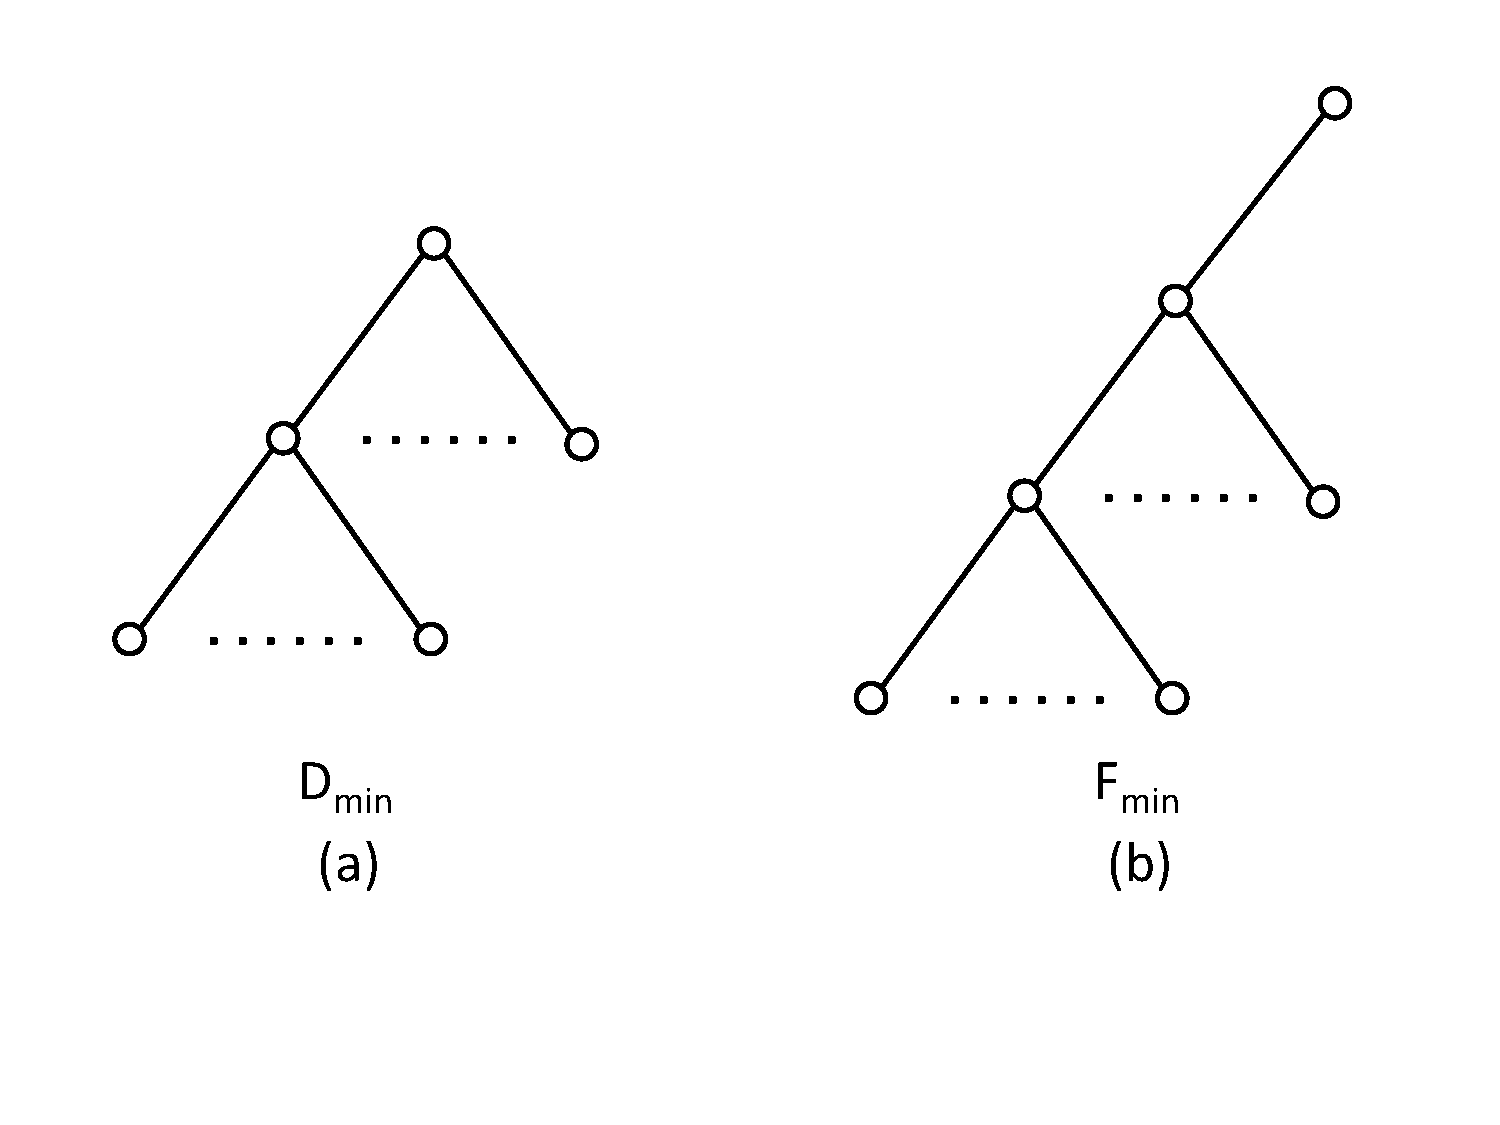
\includegraphics[scale=0.4]{../figures/fig3-5.pdf}
        \vspace{-40pt}
\caption{The minimal trees $D_{min} \in \DD$ and $F_{min} \in \FF$}
\label{fig mini}
\end{figure}

\begin{definition}
\label{def:maximal}
A tree $D \in \DD$ and $F \in \FF$ is said to be maximal if $D$ and $F$ contains all other trees in the set $\DD$ and $\FF$ as subtrees. 
\end{definition}


\begin{remark}
\label{rmk:mini}
By definition of the minimal tree, we have  
\begin{align*}
D_{min} \subseteq D \text{ and }
%\intertext{and}
F_{min} \subseteq F,
\end{align*}
for all $D \in \DD$ and $F \in \FF$. This implies that 
\begin{align*}
\lamhpq(D_{min}) \le \lambda_{h,p,q}(D) 
\intertext{and}
\lamhpq(F_{min}) \le \lambda_{h,p,q}(F). 
\end{align*}
\end{remark}








%%%%%%%%%%%%%%%%%%%%%%%%
\subsection{Generalisation of the $\lhpq$-labelling problem to the sets $\DD$ and $\FF$}
\label{sec:general results}

In the previous studies, we solved the $L(h,1,1)$ as well as the $\lhpq$-labelling problems of complete $m$-ary trees. As the former is a special of the latter, we did not spend too much time on proofs of the $\lhpq$-labelling results. Now, instead of generalising the $L(h,1,1)$-labelling result from complete $m$-ary trees to sets $\DD$ and $\FF$, we will generalise the $\lhpq$-labelling results to these sets. The $L(h,1,1)$-labelling result can then be seen as a corollary to these results. 
\begin{corollary}
\label{cor:ub}
For any trees $D \in \DD$ and $F \in \FF$, the minimum spans of the $L(h,p,q)$-labelling are bounded by
\begin{align}
\label{upper1}
\lambda_{h,p,q}(D) &\le (2\Delta -3)p+ h\\
\intertext{and}
\label{upper2}
\lambda_{h,p,q}(F) &\le (2\Delta-2)p + h. 
\end{align} 
Moreover, these bounds are the least upper bounds for $\lamhpq$ values. 
\end{corollary}

\begin{proof}
It is easy to see that these upper bounds are indeed the smallest possible, as $\TT^{(2)} \subsetneq \DD$ and $\TT^{(\ge 3)} \subsetneq \FF$ are proper subsets. If these bounds could be decreased, we would contradict Theorem \ref{thm:hpq}. 

By definitions of  the sets $\DD$ and $\FF$, we have the height of any tree $D \in \DD$ is no less than $2$, and the height of any tree $F \in \FF$ is no less than $3$. Now, substituting $m = \Delta-1$ into Theorem \ref{thm:hpq} the result is 
\begin{align}
\lambda_{h,p,q}(\tmk) = 
 \begin{cases}
 (2\Delta-3)p + h & \text{ for } k=2, \\
 (2\Delta-2)p + h & \text{ for } k \ge 3. 
 \end{cases}
\end{align} 
By Corollary \ref{cor:subtree}, we then get 
\begin{align*}
%\label{ubforD}
\lambda_{h,p,q}(D) &\le 
 \begin{cases}
 (2\Delta-3)p + h  & \text{ for } hei(D) = 2, \\
 (2\Delta-2)p + h & \text{ for } hei(D) \ge 3. 
 \end{cases} \\
\intertext{and}
\lambda_{h,p,q}(F) &\le (2\Delta-2)p + h, \forall F \in \FF. 
\end{align*} 

It remains to show that the upper bound can be decreased by $p$ when $hei(D) \ge 3$; i.e., $\lambda_{h,p,q}(D) \le (2\Delta-3)p+h$, for $hei(D) \ge 3$. 

Notice that for a tree $D \in \DD$ with $hei(D) \ge 3$, we must not have $\Delta_2(D) = 2\Delta$. This is due to the definition of the set $\DD$. Hence, the maximal tree $D_{max}$ must satisfy the following property: 
\begin{enumerate}[(*)]
\item for any heavy edge $uv \in E(D)$, we must have $d(u) = \Delta, d(v) = \Delta-1$ or $d(v) = \Delta, d(u) = \Delta-1$. 
\end{enumerate}

The upper bound $(2\Delta-2)p+h$ comes from Theorem \ref{thm:hpq} for complete $m$-ary tree $\tmk$ with $k \ge 3$. We have proved that to $L(h,p,q)$-label $\tmk$, we alternatively assign label sets $S_1=[0,m]p$ and $S_2=(mp+h)+[0,m]p$ to sets of vertices in each depth. But for the tree $D_{max}$, each set of vertices with either even or odd depth has one element less than those in $\tmk$ by property (*). Thus we can delete a label from label set $S_1$ or $S_2$. In either case, the minimum span is reduced by $p$. For example, if $D_{max}$ is as shown in Fig. \ref{ex D 1}, then we use the following label sets: 
\begin{itemize}
\item $S_1' = [0, m-1]p$; 
\item $S_2' = (m-1)p+h+[0,m]p$. 
\end{itemize}
If $D_{max}$ is as shown in Fig. \ref{ex D 11}, then we use the following label sets: 
\begin{itemize}
\item $S_1=[0,m]p$;
\item $S_2''=mp+h+[0,m-1]p$. 
\end{itemize}

\begin{figure}
 \centering
      \vspace{-5pt}
    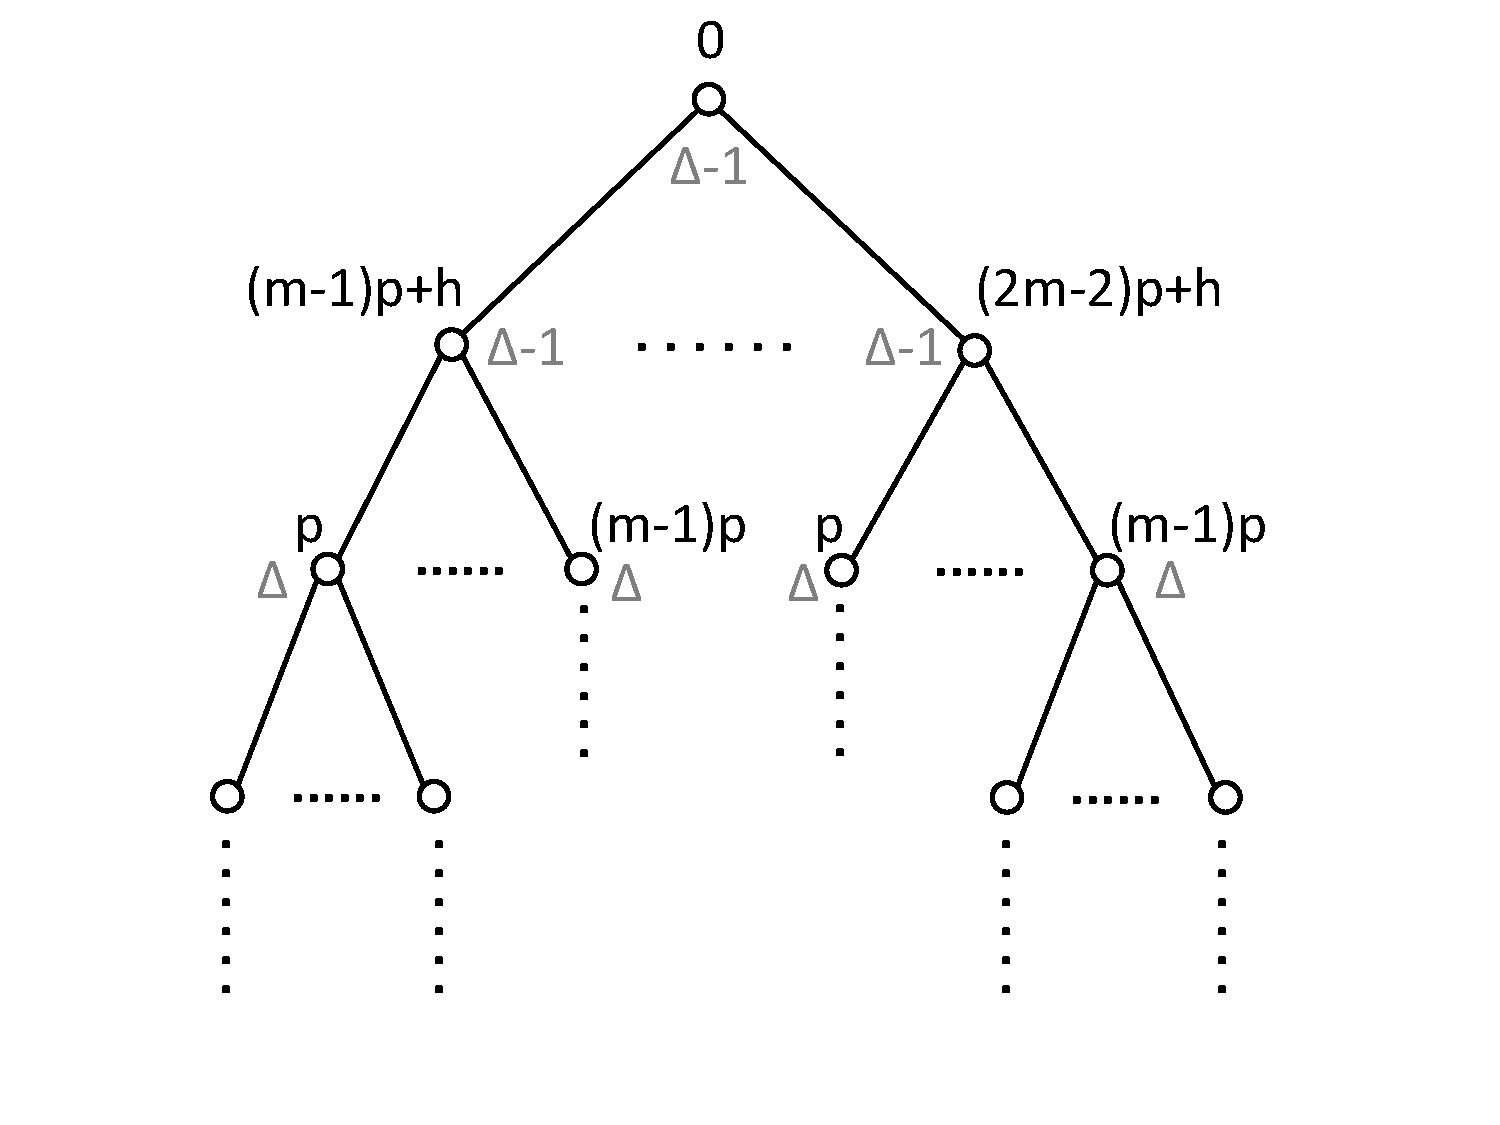
\includegraphics[scale=0.4]{../figures/fig3-6-a.pdf}
        \vspace{-0pt}
\caption{The $\lhpq$-labelling of $D_{max}$}
\label{ex D 1}
\end{figure}

\begin{figure}
 \centering
      \vspace{-20pt}
    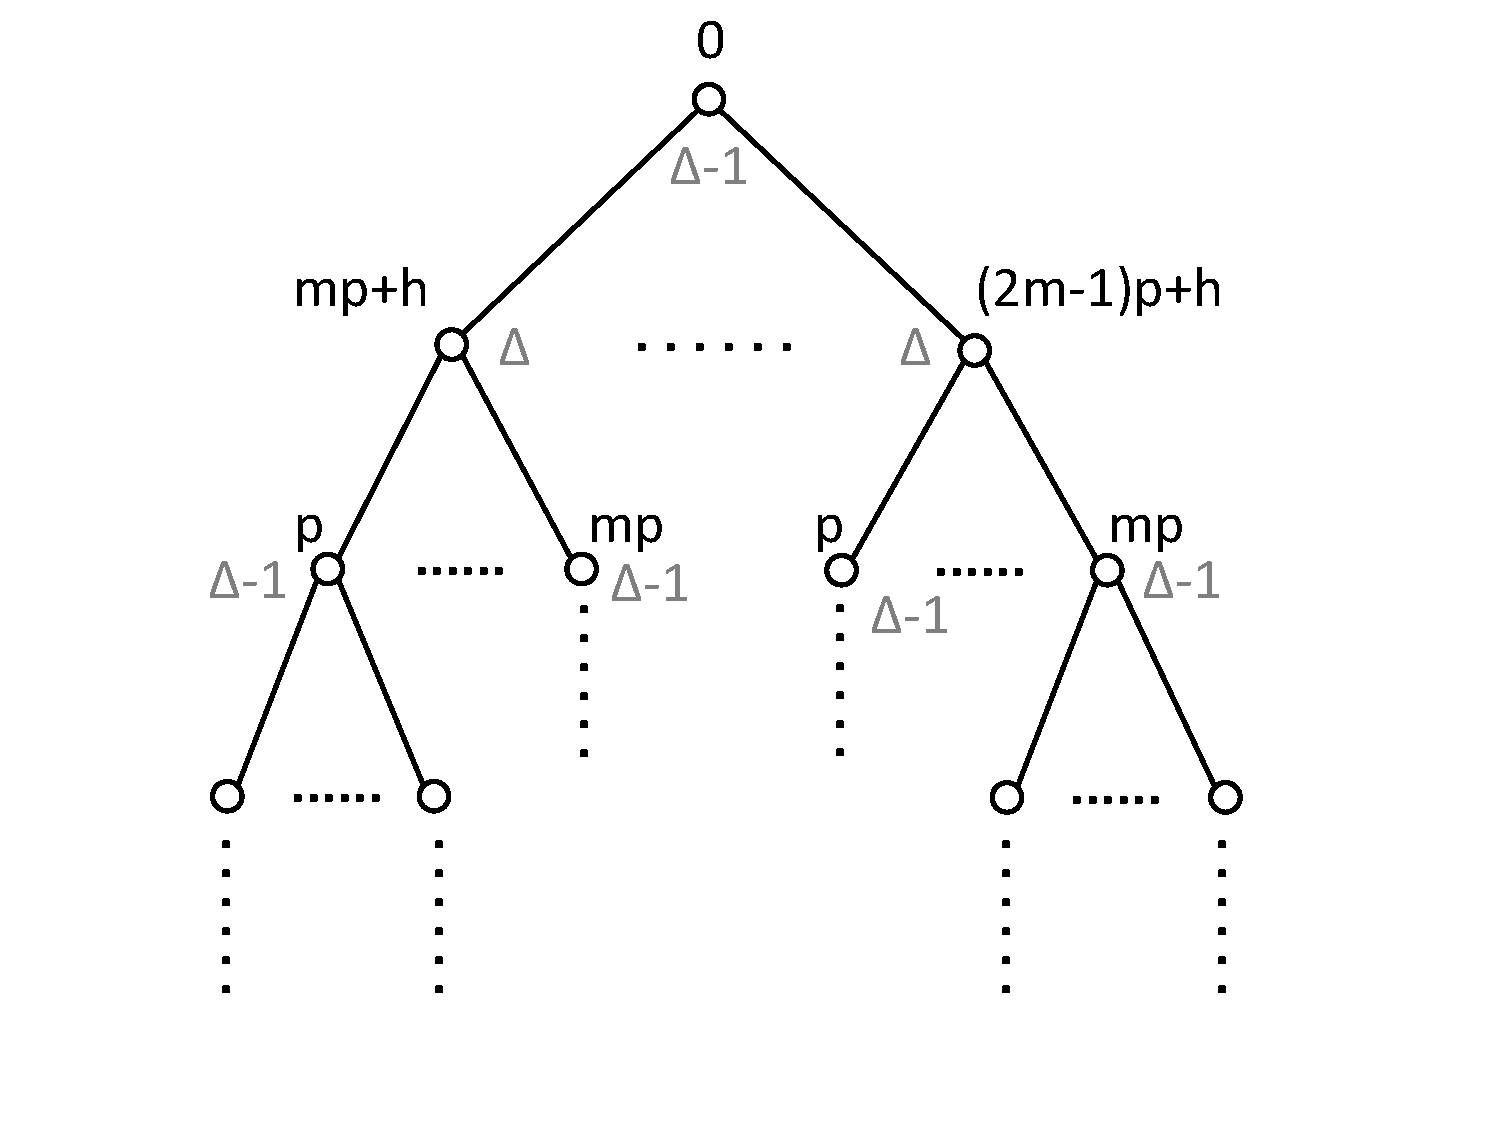
\includegraphics[scale=0.4]{../figures/fig3-6-b.pdf}
        \vspace{-0pt}
\caption{The $\lhpq$-labelling of $D_{max}$}
\label{ex D 11}
\end{figure}


By using these label sets, we showed that when $hei(D) \ge 3$, there exists a map that $L(h,p,q)$-labels $D$ with minimum span $\lambda_{h,p,q}(D) = (2m-1)p+h=(2\Delta-3)p+h$. Thus the corollary is proved.  
\end{proof}
\qed

The following two theorem gives upper and lower bounds for $\lamhpq(D)$ and $\lamhpq(F)$. 

\begin{theorem}
\label{thm:h11forD}
For any tree $D \in \DD$, the minimum span of the $\lhpq$-labelling is bounded by the following:
\begin{align*}
\max\{(2\Delta - 3)p+q, (\Delta-1)p+h\} \le \lambda_{h,p,q}(D) \le (2\Delta-3)p + h. 
\end{align*}
\end{theorem}

The value $(2\Delta-2)p+q$ is achieved for $(\Delta-2)p+q \ge h$, while $(\Delta-1)p+h$ is achieved for $(\Delta-2)p+q \le h$. 
\begin{proof}
The upper bounds have been verified by Corollary \ref{cor:ub}. it remains to prove the lower bound case by case. Remark \ref{rmk:mini} shows that $\lamhpq(D_{min}) \le \lamhpq(D)$ for all $D \in \DD$, where $D_{min} \in \DD$ is defined as the minimal tree. Thus we just need to find the $\lamhpq$  values for $D_{min}$ in each particular case. 

If $(\Delta-2)p+q \ge h$, consider $D_{min}$ with $d(u) = \Delta-1, d(v) = \Delta$. Let $f:V(D_{min}) \rightarrow [0, \infty)$ be a function, such that $f(N(v)) = [0,\Delta-1]p$ with $f(u) = 0$ and $f(N(u))=(\Delta-1)p+q+[0,\Delta-2]p$ with $f(v) = (2\Delta-3)p+q$. Then $f$ is an $L(h,p,q)$-labelling of $D_{min}$ with $span(f) = (2\Delta-3)p+q$. (Fig. \ref{ce2} (a))

If $(\Delta-2)p+q \le h$, then the function $f: V(D_{min}) \rightarrow [0,\infty)$ labels $D_{min}$ in the following way: $f(N(v))=[0,\Delta-1]p$ and $f(N(u))=p+h+[0,\Delta-2]p$ such that $f(u)=0$ and $f(v) = (\Delta-1)p+h$. Clearly, the function $f$ is again an $L(h,p,q)$-labelling of $D_{min}$ with $span(f) = (\Delta-1)p+h$. (Fig. \ref{ce2} (b))
\begin{figure}
\centering
      \vspace{-15pt}
    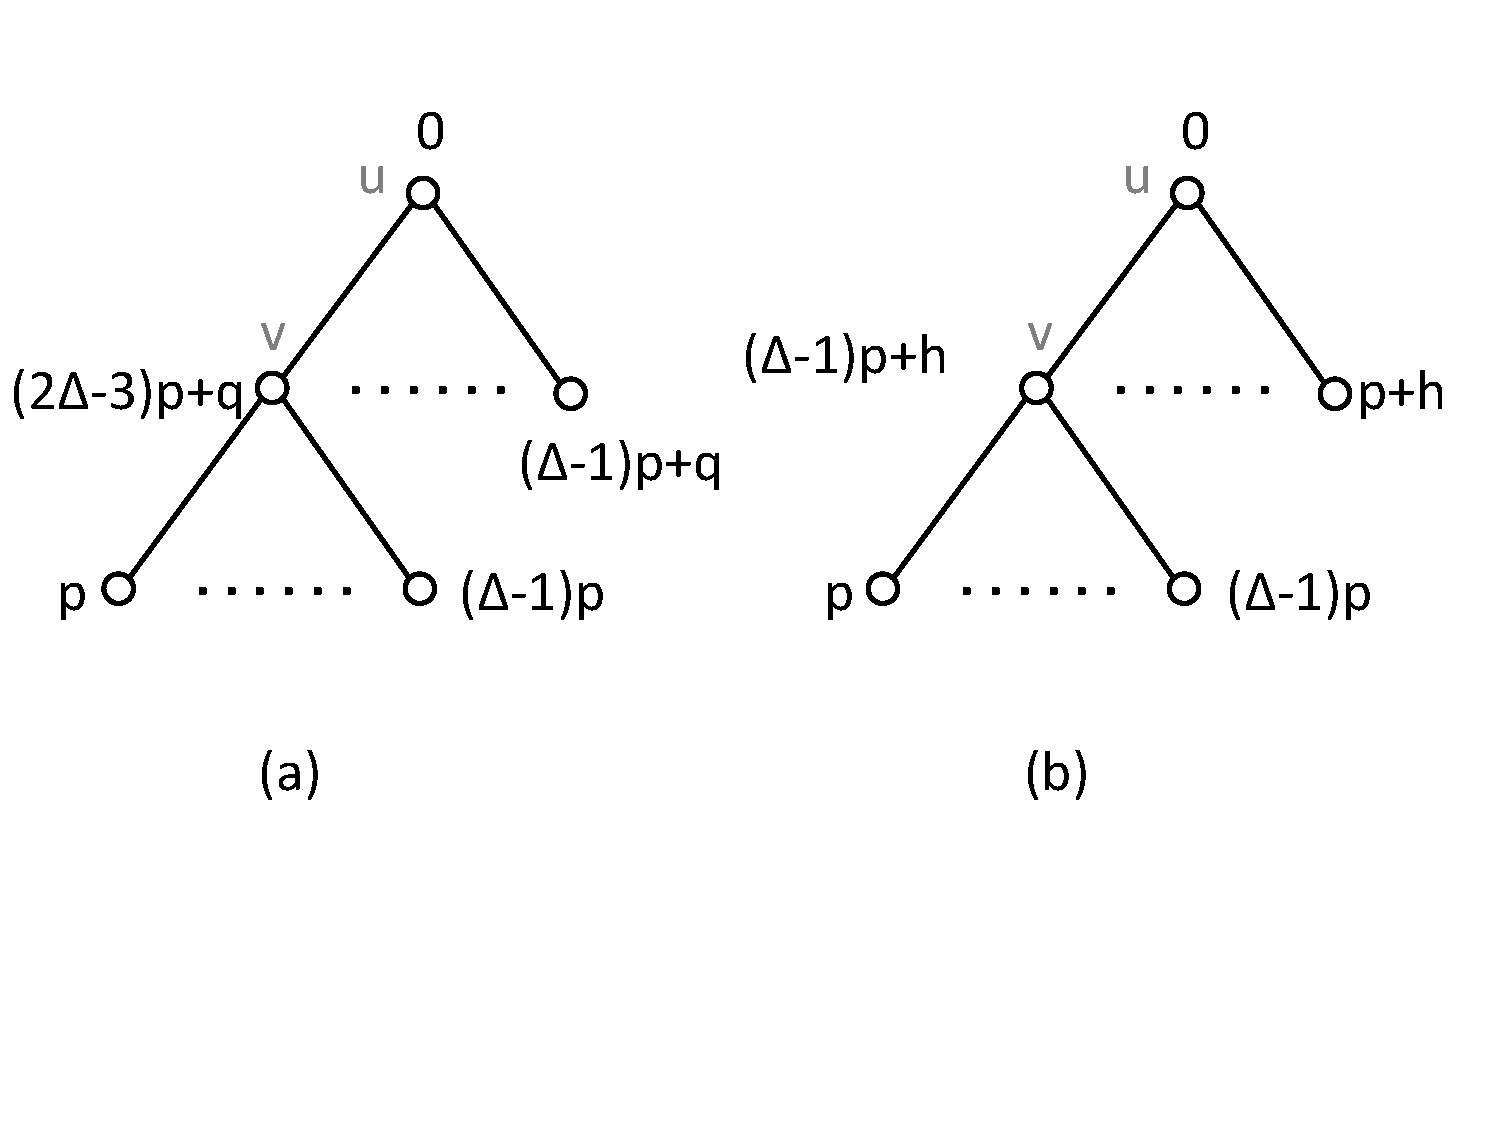
\includegraphics[scale=0.4]{../figures/fig3-7.pdf}
        \vspace{-60pt}
\caption{The $\lhpq$-labelling of $D_{min}$ with span equals $\max\{(2\Delta - 3)p+q, (\Delta-1)p+h\}$}
\label{ce2}
\end{figure}
\end{proof}
\qed

\begin{theorem}
\label{thm:h11forF}
For any tree $F \in \FF$, the minimum span of the $\lhpq$-labelling is bounded by 
\begin{align*}
\max\{(2\Delta - 2)p+q, (\Delta-1)p+h\} &\le \lambda_{h,p,q}(F) \le (2\Delta-2)p + h.
\end{align*} 
\end{theorem}

Again, the value $(2\Delta - 2)p+q$ is achieved for $(\Delta-1)p+q \ge h$, while $(\Delta-1)p+h$ is achieved for $(\Delta-1)p+q \le h$. 
\begin{proof}
The proof is similar to the proof of Theorem \ref{thm:h11forD}. We only need to prove the lower bound, as the upper bound has been proved by Corollary \ref{cor:ub}. 

Again, we solve $\lamhpq(F_{min})$ for the minimal tree $F_{min} \in \FF$. Consider a function $f:V(F_{min}) \rightarrow [0,\infty)$ such that $F_{min}$ is labelled as follows.(Fig. \ref{ce4}). 

If $(\Delta-1)p+q \ge h$, then
\begin{itemize}
\item $f\left(N(v)\right) = [0, \Delta-1]p$ such that $f(u)=0$;
\item $f\left(N(u)\right) = (\Delta-1)p+q+[0,\Delta-1]p$ such that $f(v) = (2\Delta-2)p=q$. 
\end{itemize}

If $(\Delta-1)p+q \ge h$, then 
\begin{itemize}
\item $f\left(N(v)\right) = [0, \Delta-1]p$ such that $f(u) = 0$; 
\item $f\left(N(u)\right) = h+[0,\Delta-1]p$ such that $f(v) = (\Delta-1)p+h$. 
\end{itemize}

\begin{figure}
\centering
      \vspace{-10pt}
    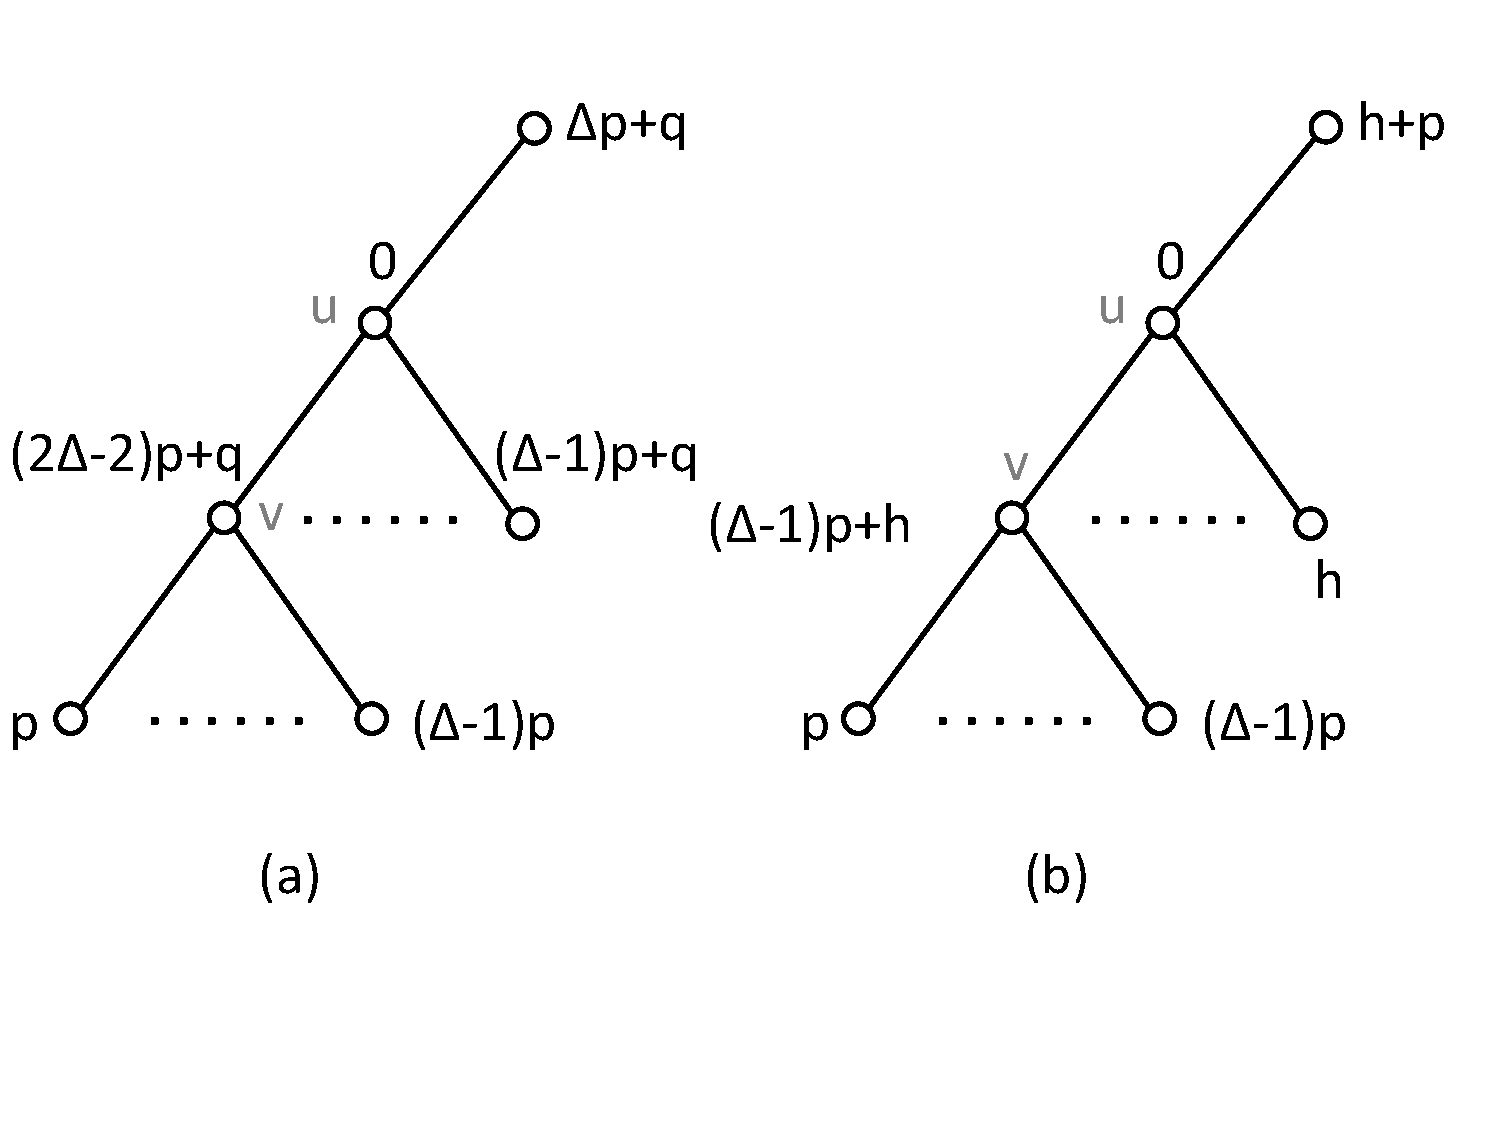
\includegraphics[scale=0.4]{../figures/fig3-8.pdf}
        \vspace{-40pt}
\caption{The $\lhpq$-labelling of $F_{min}$ with span equals $\max\{(2\Delta - 2)p+q, (\Delta-1)p+h\}$} 
\label{ce4}
\end{figure}

It can be seen that $F_{min}$ is $L(h,p,q)$-labelled by the function $f$ with $span(f) = \max\{(2\Delta - 2)p+q, (\Delta-1)p+h\}$. This completes the proof of Theorem \ref{thm:h11forF}. 
\end{proof}
\qed





%%%%%%%%%%%%%%%%%%%%%%%%%%%%%%%%%%%

\subsection{The set of trees with $T_{m,2}$ as a local structure}
\label{subsection:tm2}

Define the set 
\[
\KK :=\{ T \mid T_{m,2} \subseteq T \text{ is a subtree }, m = \Delta-1\}
\]
where $T_{m,2}$ is a complete $m$-ary tree with height $2$. We can partition this set into two subsets
\[
\KK = \KK_{2\Delta} \cup \KK_{2\Delta-1}
\]
where
\begin{align*}
\KK_{2\Delta-1} &:= \{ T \in \KK \mid \Delta_2(T) = 2\Delta-1\}, \\
\KK_{2\Delta} &:= \{T \in \KK \mid \Delta_2(T) = 2\Delta\}. 
\end{align*}

\begin{corollary} 
For a tree $T \in \KK$, we have the minimum span of the $\lhpq$-labelling of $T$ is
\begin{align}
\label{eq:two sets3}
\lambda_{h,p,q}(T) = 
 \begin{cases}
 (2\Delta-3)p+h & \text{ for } T \in \KK_{2\Delta-1}, \\
 (2\Delta-2)p+h \text{ or } (2\Delta-3)p+h & \text{ for } T\in \KK_{2\Delta}. 
 \end{cases}
\end{align}
\end{corollary}

\begin{proof}
By definition, we have $\KK_{2\Delta-1} \subsetneq \DD$ and $\KK_{2\Delta} \subsetneq \FF$ are proper subsets of $\DD$ and $\FF$. Corollary \ref{cor:ub} then implies $\lamhpq(T) \le (2\Delta-3)p+h,$ when $T\in \KK_{2\Delta-1}$ and $\lamhpq(T) \le (2\Delta-2)p+h,$ when $T \in \KK_{2\Delta}$. 

On the other hand, we have proved that $\lamhpq(\tm2) = (2m-1)p+h = (2\Delta-3)p+h$. As $T_{m,2}$ is a subtree of every tree in sets $\KK_{2\Delta}$ and $\KK_{2\Delta-1}$, $\lamhpq(\tm2)$ can be used as the lower bound of $\lamhpq(T)$ for $T \in \KK$. This implies \eqref{eq:two sets3}. 
\end{proof}
\qed

Notice that $\TT^{(2)} \subsetneq \KK_{2\Delta-1}$ and $\TT^{(\ge 3)} \subsetneq \KK_{2\Delta}$ are also proper subsets of $\KK_{2\Delta-1}$ and $\KK_{2\Delta}$ respectively. There are some trees in the complement $\KK_{2\Delta-1} \setminus \TT^{(2)}$and $\KK_{2\Delta} \setminus \TT^{(\ge 3)}$. By the above corollary, we know that every tree $T \in \KK_{2\Delta-1}$ has $\lambda_{h,p,q}(T)= (2\Delta-3)p+h$. However, not every tree $T \in \KK_{2\Delta}$ has the same $\lambda_{h,p,q}$ value. Hence, we would like to characterise the set $\KK_{2\Delta}$ such that we can decide the $\lamhpq$ value of any tree in this set by simply looking at its structure.

\begin{proposition}
\label{character}
For any tree $T \in \KK_{2\Delta} \setminus \TT^{(\ge 3)}$, we have $\lambda_{h,p,q}(T) = (2\Delta-2)p+h$ if and only if $T' \subsetneq T$ is a proper subtree of $T$, where $T' := T_{m,2} + \{uv\}$ is a complete $m$-ary tree with height $2$ plus an extra edge attached to its root $u$. 
\end{proposition}

\begin{proof}
Suppose $T$ contains a proper subtree $T'$ defined as above. Theorem \ref{thm:hpq} proves that $\lambda_{h,p,q}(T_{m,2}) = (2m-1)p+h = (2\Delta-3)p+h$. By attaching an extra edge onto the root of $T_{m,2}$, the cardinality of the original label set is increased by $p$. Moreover, the resulting label set is still sufficient to $\lhpq$-label the tree $T'$. This implies $\lambda_{h,p,q}(T') = (2\Delta-2)p+h$. As $T' \subseteq T$ is a proper subtree of $T$, it follows that $\lambda_{h,p,q}(T) = (2\Delta-2)p+h$ for any tree $T \in \KK_{2\Delta} \setminus \TT^{(\ge 3)}$. 

Conversely, if $\lambda_{h,p,q}(T) = (2\Delta-2)p+h$, we need to show $T$ must contain $T'$ as a subtree. It is equivalent to show that if $T$ does not contain $T'$ as a subtree, then $\lambda_{h,p,q}(T) = (2\Delta-3)p+h$. 

Now, let us focus on the local structure $T_{m,2}$. By definition of the set $\KK_{2\Delta}$, every tree in $\KK_{2\Delta}$ contains $T_{m,2}$ as a subtree. Let us denote the root of $T_{m,2}$ by $u_0$, the children of $u_0$ by $\{u_i \mid i \in [1,m]\}$, and grandchildren by $\{u_{ij} \mid i, j \in [1,m]\}$. The assumption $T' \not\subseteq T$ ensures that there is only one subtree of $T$ that has the structure of $\tm2$, and this $\tm2$ has to stay on the top of $T$, that is, $u_0$ is the root of both $\tm2$ and $T$. 

In fact, we can construct the maximal tree $T_{max} \in  \KK_{2\Delta} \setminus \TT^{(\ge 3)}$, where $T_{max}$ contains only one $\tm2$ as a subtree, from $\tmk \in \TT^{(\ge 3)}$ by doing the following step recursively: 
\\
\\
\fbox{
\parbox{\linewidth}{
\begin{enumerate}[(*)]
\item For a vertex $\uij \in V(\tmk)$ with $k \ge 3$ and $card(0\dots ij) \ge 1$, if $d(\uij) = m+1$ then delete one vertex $u \in G(\uij)$ from the grandchildren set, and the corresponding branch attached to $u$; if $d(\uij) < m+1$ then do nothing. 
\end{enumerate}
}
}
\\
\\
The grandchildren set is $G(u):=\{v \in V(T) \mid d(u,v) = 2, dep(u) = dep(v) -2\}$. Clearly, by deleting vertices from $\tmk \in \TT^{(\ge 3)}$ recursively using the above step, we get a tree $T \in \KK_{2\Delta} \setminus \TT^{(\ge 3)}$ such that there exits only one subtree $\tm2 \subseteq T$. 

For the tree $T_{max}$ constructed using the above step, we need to show that $\lamhpq(T_{max}) = (2\Delta-3)p+h$. If we can show this, then it follows that $\lamhpq(T) \le \lamhpq(T_{max})$, for all $T \in \KK_{2\Delta} \setminus \TT{(\ge 3)}$. To do this, we need to modify the $L(h,p,q)$-labelling of complete $m$-ary trees $\tmk$ with $k\ge 3$, which we defined in Section 3.5. Let $S_1 := [0,m]p, S_2 := mp+h+[0,m-1]p$, then 
\begin{itemize}
\item $f(u_0) = 0$;
\item $\{f(u_i) \mid i \in [1,m]\} = S_2$ such that $f(u_i) = (m+i-1)p+h$;
\item $f(C_{u_{0 \dots ijk}}) =
 \begin{cases}
 \SS_1 \setminus f(P(u_{0 \dots ijk})) & \text{ if } d(u_0, u_{0\dots ijk}) \\ &\text{ is odd, } \\
 (\SS_2 \cup \{2mp+h\}) \setminus f(P(u_{0 \dots ijk})) & \text{ if } d(u_0, u_{0\dots ijk}) \\ &\text{ is even and } 
 \\ &f(\uijk)=m, \\
  (\SS_2 \cup \{(m-1)p+h\}) \setminus f(P(u_{0 \dots ijk})) & \text{ if } d(u_0, u_{0\dots ijk}) \\ &\text{ is even and } \\ &f(\uijk) \neq m.
 \end{cases}$
\end{itemize}

If we $L(h,p,q)$-label complete $m$-ary trees $\tmk \in \TT^{(\ge 3)}$ and delete some vertices using (*) in a certain way, then  the resulted tree $T \in \KK_{2\Delta} \setminus \TT^{(\ge 3)}$ is $L(h,p,q)$-labelled with minimum span $\lamhpq(T) = (2\Delta-3)p+h$.  Precisely, the following is how to delete vertices from $\tmk$ using (*). 

Suppose $\tmk \in \TT^{(\ge 3)}$ is $L(h,p,q)$-labelled by a function $f$ with $\lamhpq(\tmk) = (2\Delta-3)p+h$. For any vertex $\uij \in V(\tmk)$ and $card(0\dots ij) \ge 1$, do the following steps from top to bottom of $\tmk$, start from the level of vertices with depth $2$:
\begin{enumerate}[(i)]
\item if $d(\uij) = m+1$, then delete the vertex $u \in G(\uij)$, where $f(P(u)) = mp$ and $f(u) = 2mp+h$. 
\item for any vertex $\uijk$ in the next level, if $d(\uijk) = m+1$, then delete the vertex $v \in G(\uijk)$, where $f(v) = mp$; if $d(\uijk) < m+1$ then do nothing. 
\end{enumerate}

Clearly after deletion of vertices from $\lhpq$-labelled complete $m$-ary trees, the resulted tree $T \in \KK_{2\Delta} \setminus \TT^{(\ge 3)}$ is still $L(h,p,q)$-labelled. More importantly, the above steps delete all vertices bear the maximum label $2mp+h$, so we have minimum span $\lamhpq(T) = (2m-1)p+h=(2\Delta-3)p+h$. This completes the proof of this proposition. 
\end{proof}
\qed

So far in this chapter, we have bound for the minimum span of $L(h,1,1)$ as well as $\lhpq$-labelling  of complete $m$-ary trees. These values also help us to get tight ranges of $\lamhpq$ values of some general sets of trees that contain complete $m$-ary trees. 

In the next chapter, we will move onto the second major topic, the cyclic metric labelling problem. 
\chapter{Cyclic metric labelling problem}

In this section, we turn our attention for the linear metric labelling problem to the cyclic metric $C(p_1, p_2, p_3)$-labelling problem. The class of trees we will study is still the class of complete $m$-ary trees. For our convenience, we again let the parameters $p_1=h,p_2=p, p_3=q$. In particular, we will start with the case when $p_2 = p_3 = 1$ first.  

The structure of this chapter is the same as Chapter 3. We start off with definitions and corresponding notation for the cyclic metric labelling problem. In Section 4.2, we give some known results in this area. This contains cyclic metric labelling of various graphs. In the following section, we present our results; i.e.,  the $\chpq$-labelling of complete $m$-ary trees. In the last part of this chapter, we will generalise some of these results to sets $\DD, \FF$ and $\KK$.  


\section{Definitions and notation}

Recall that we use $d(u,v)$ to denote the distance between two vertices $u$ and $v$ of a graph $G$, where distance is defined as the length of the shortest path between $u$ and $v$ in $G$. We call a path with two identical ends a cycle. A cycle with length $n$ is called a $n$-cycle, denoted by $C^n$. 

\begin{definition}
\label{labelled cycle}
Let $f:[0,n-1] \rightarrow V(C^n)$ be a bijective function that assigns non-negative integers to vertices of $C^n$ anti-clockwise in numerical order. We say $C^n$ is a labelled $n$-cycle if there exits such a map $f$. 
\end{definition}

\begin{corollary}
\label{cor:mod}
For any two vertices $u, v \in V(C^n)$ of a labelled $n$-cycle, the distance between $u$ and $v$ is 
\[
d_{C^n}(u, v) = \min \left\{u-v, v-u\right\} \pmod {n}.
\]
\end{corollary}

\begin{proof}
The distance between two vertices is defined to be the length of the shortest path between these two vertices. For $u, v \in V(C^n)$, there are exactly two paths $P_{uv}$ and $P_{vu}$ in $C^n$. Thus we have $d_{C^n}(u,v) = \min\{l(P_{uv}), l(P_{vu})\}$. As $C^n$ is a labelled $n$-cycle, vertices $u,v$ bear non-negative integers from the label set $[0, n-1]$. Then $l(P_{uv}) = v-u \pmod{n}$ and $l(P_{vu}) = u-v \pmod{n}$. This proves the corollary. 
\end{proof}
\qed

\begin{example}
$C^5$ is a $5$-cycle such that each vertex $v_i$ bears the label $i$, for $i \in [0, 4]$. (Fig. \ref{cyclic distance}). By Corollary \ref{cor:mod}, the distance between vertices $v_0$ and $v_3$ on $C^5$ is 
\begin{align*}
d(v_0,v_3) &= \min \left\{ 0-3, 3-0\right\} \pmod 5\\
&= \min\{2, 3\}\\
&= 2.
\end{align*}
\\
\\
\\
\begin{figure}
  \centering
      \vspace{-20pt}
    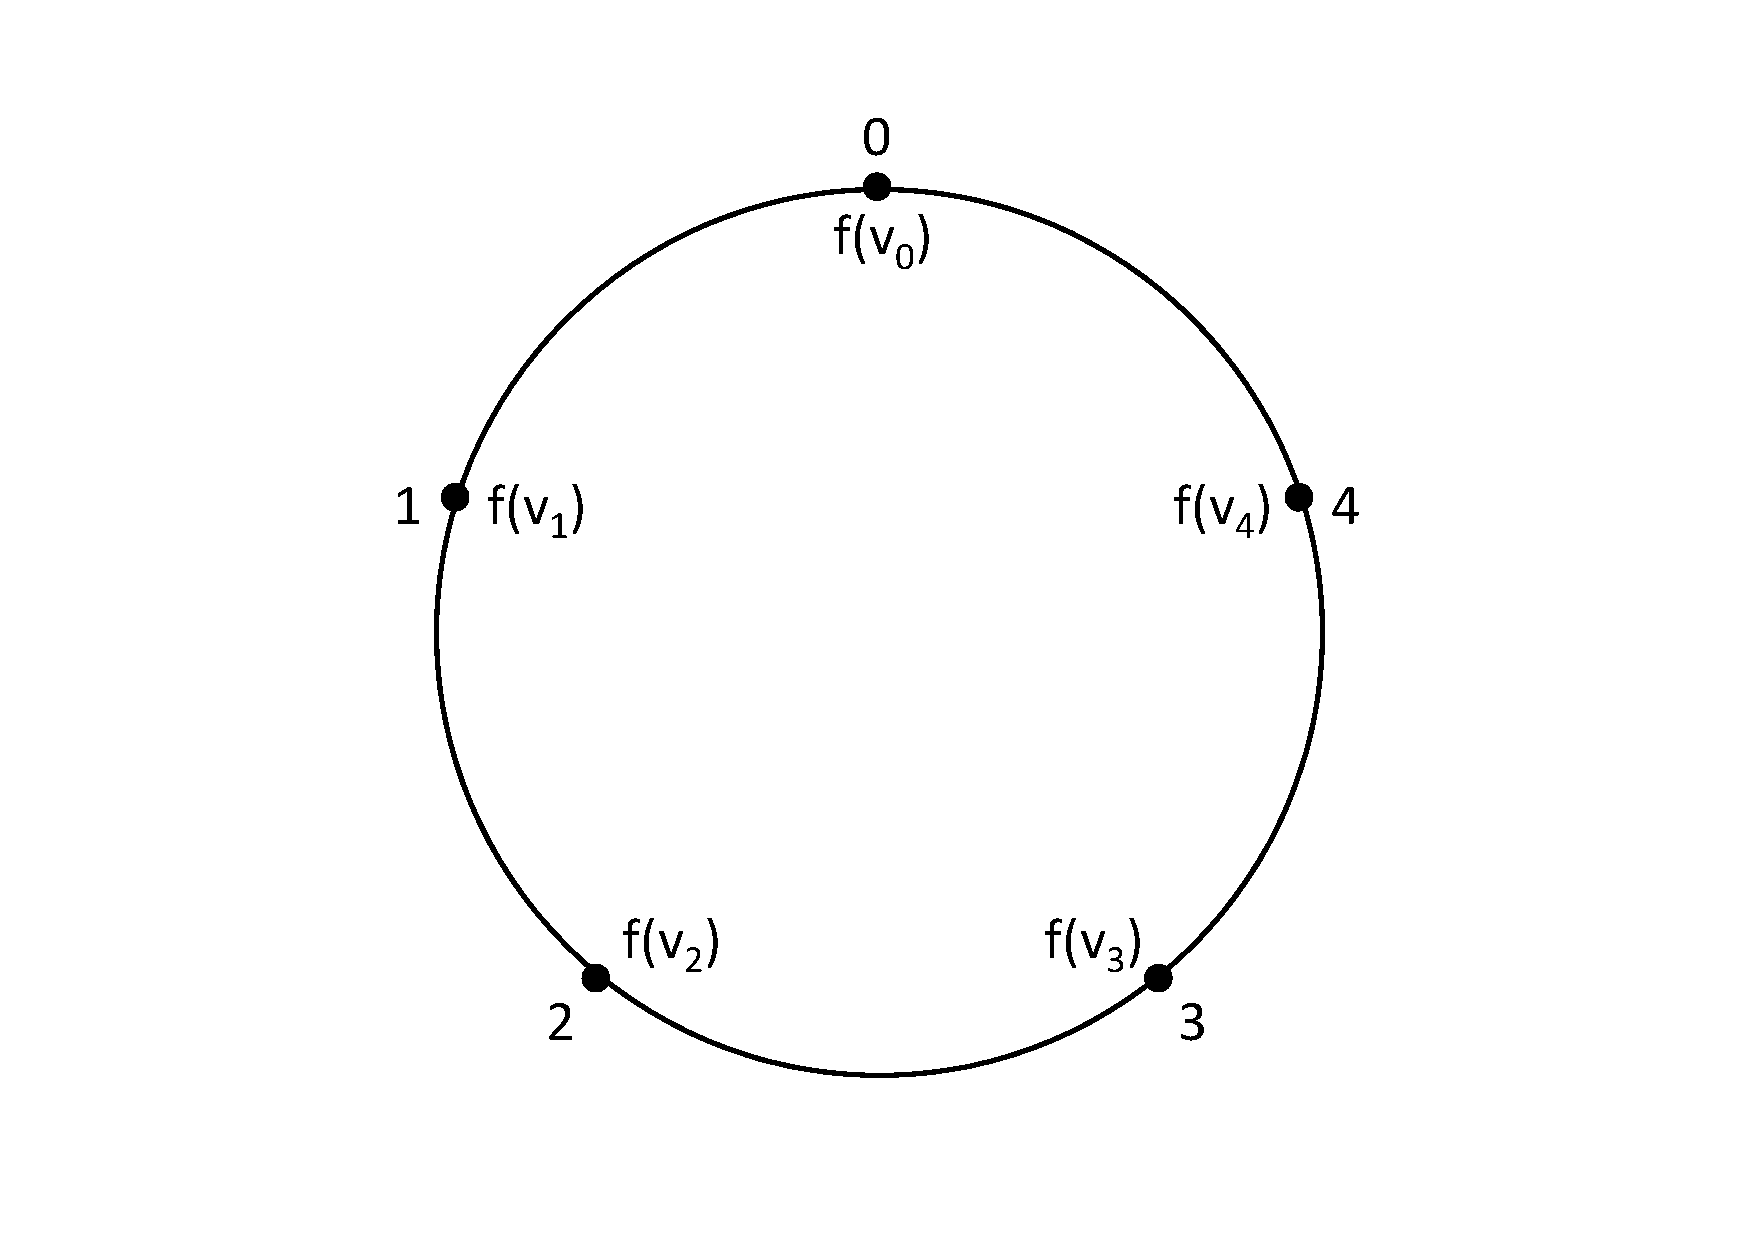
\includegraphics[scale=0.4]{../figures/fig4-1.pdf}
        \vspace{-20pt}
  \caption{Example of cyclic distance}
  \label{cyclic distance}
\end{figure}
\end{example}

\begin{definition}
\label{def:cyclic1}
A cyclic metric $C(p_1, p_2, p_3, \dots)$-labelling of a graph $G$ is a map 
\[
f : V(G) \rightarrow V(C^n) 
\] 
from vertices of $G$ to vertices of a labelled $n$-cycle $C^n$ such that
\[
|\min\{f(u)-f(v), f(v) - f(u)\}| \ge p_{i}\pmod{n}, \text{ if } d_{G}(u, v) = i, \forall i \in [1, \infty) 
\]
where $n \ge 2$ is an integer.  
\end{definition}
\begin{example}
Fixing $C^n$ to be a $5$-cycle; i.e.,  $n = 5$. We can see that Fig. \ref{cyclic labelling} (a) is an $L(2,1,1)$-labelling of $T_{2,2}$, but not a $C(2,1,1)$-labelling, since $|f(u_0) - f(u_2)| = 1 \pmod{6}$ while $d(u_0, u_1) = 1$. Fig. \ref{cyclic labelling} (b) is a $C(2,1,1)$-labelling of $T_{2,2}$. 
\begin{figure}
 \centering
      \vspace{-10pt}
    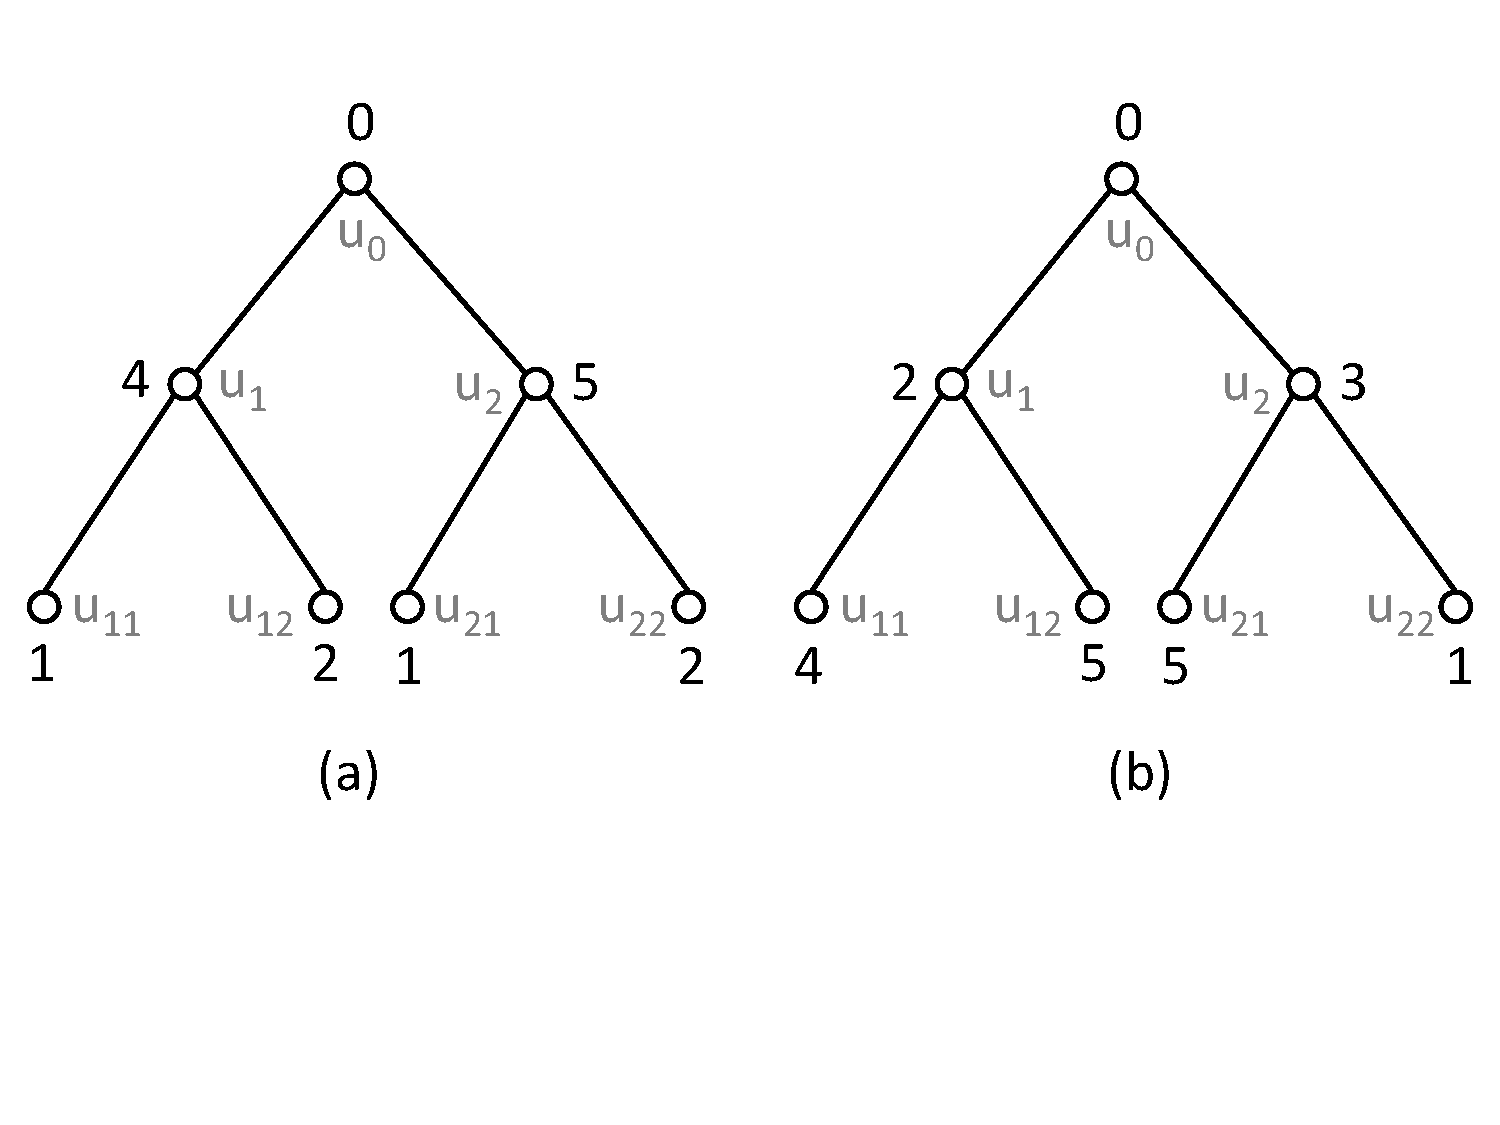
\includegraphics[scale=0.4]{../figures/fig4-2.pdf}
        \vspace{-50pt}
 \caption{Example of $C(2,1,1)$-labelliings of $T_{2,2}$}
  \label{cyclic labelling}
\end{figure}
\end{example}

The aim of cyclic metric labelling problem is to minimise the maximum label used. According to Definition \ref{def:cyclic1}, the objective is to find the smallest integer $n$ for the $n$-cycle that satisfies the above constraint. The $C(p_1, p_2, p_3, \dots)$-labelling is similar to $L(p_1, p_2, p_3, \dots)$-labelling, except this time the function $f$ maps vertices of a graph to vertices of a labelled cycle rather than a path. Of course as there is a unique path between any two vertices on a path, the $L(p_1, p_2, p_3, \dots)$-labelling problem is relatively easier. But the related concepts are still the same as those for linear metric labelling problem.

If a graph $G$ is $C(p_1, p_2, p_3, \dots)$-labelled by a function $f$, then the \emph{span} of the function $f$, $span(f)$, is said to be the difference between the maximum and minimum used labels. Precisely, 
\[
span(f) = \max\{f(u) \mid \forall u \in V(G)\} - \min\{f(u) \mid \forall u \in V(G)\}.
\]
The \emph{minimum span} of $C(p_1, p_2, p_3, \dots)$-labelling of the graph $G$ is then defined as the minimum among all possible $span(f)$. To distinguish it from the minimum span $\lambda_{p_1, p_2, p_3, \dots}(G)$, we use $\t_{p_1, p_2, p_3, \dots}(G)$ to denote the minimum span of $C(p_1, p_2, p_3, \dots)$-labelling of $G$.

%{\bf Technique:}
%Note that when dealing with cyclic metric labelling on complete $m$-ary trees in this chapter, we will not use the technique that we used in the previous chapter. That is, directly finding an optimal labelling on a complete $m$-ary tree $T$, which satisfies the $L(h1,1,)$-labelling constraint. Instead, we will fix a labelled cycle $H$, and try to map vertices of $T$ to vertices of $H$. Since once we can find such a way to map vertices of $T$ to labels of $H$, then we can use the inverse function to map labels of $H$ back to vertices of $T$. 
\begin{corollary}
\label{cor:compare}
For a graph $G$ with $diam(G) \ge 3$, if $\lamhpq(G)$ and $\t_{h,p,q}(G)$ are the minimum spans of the $L(h,p,q)$ and $C(h,p,q)$-labelling of $G$ respectively, then 
\begin{align*}
\lambda_{h,p,q}(G) \le \t_{h,p,q}(G).
\end{align*} 
\end{corollary}

\begin{proof}
This corollary follows from the definition of cyclic metric labelling naturally. If we have the graph $G$ is both $\chpq$ and $\lhpq$-labelled with the minimum spans $\thpq(G) < \lambda_{h,p,q}(G)$, then by deleting the edge between $0$ and $\t_{h,p,q}(G)$ on the labelled $n$-cycle $C^n$ we get another function, which $\lhpq$-labels $G$ with a smaller minimum span. This contradicts the assumption that $\lambda_{h,p,q}(T)$ is the minimum span.  
\end{proof}
\qed

When mapping vertices of a graph to a labelled path, we always start from the label $0$ as we aim for achieving the smallest maximum label. However, when mapping them to a labelled cycle, there is no fixed starting point, as there is no difference between starting from label $0$ or $1$. The next definition defines an equivalence relation between two $C(h,p,q)$-labellings. 

\begin{definition}
\label{def:equi}
Let 
\[
f_1 : V(G) \rightarrow V(C_1^n)
\]
and
\[
f_2: V(G) \rightarrow V(C_2^n)
\]
be two different $C(h,p,q)$-labellings of a graph $G$. We say the function $f_{1}$ is equivalent to $f_{2}$ if the two labelled $n$-cycles are identical and $f_1(V(G)) = R \circ f_2(V(G))$, where $R$ is a rotation of $C^n$. 

Precisely, if $C_1^n = C_2^n$ and $f_1(V(G)) = f_2(V(G)) +r \pmod n$, where $r \in [0,n-1]$ is an integer, then the function $f_1$ is said to be equivalent to $f_2$, denoted by   $f_{1} \sim f_{2}$. 
\end{definition}

\begin{example} 
Let $f_1$ and $f_2$ be two different $C(2,1,1)$-labellings of the complete $2$-ary tree $T_{2,2}$. (Fig. \ref{fig equivalent}) It is obvious that the labelled $5$-cycles are identical. Also, $f_1(V(T_{2,2})) +2= f_2(V(T_{2,2})) \pmod 6$. Hence, the two $C(2,1,1)$-labellings are equivalent. 
\begin{figure}
  \centering
    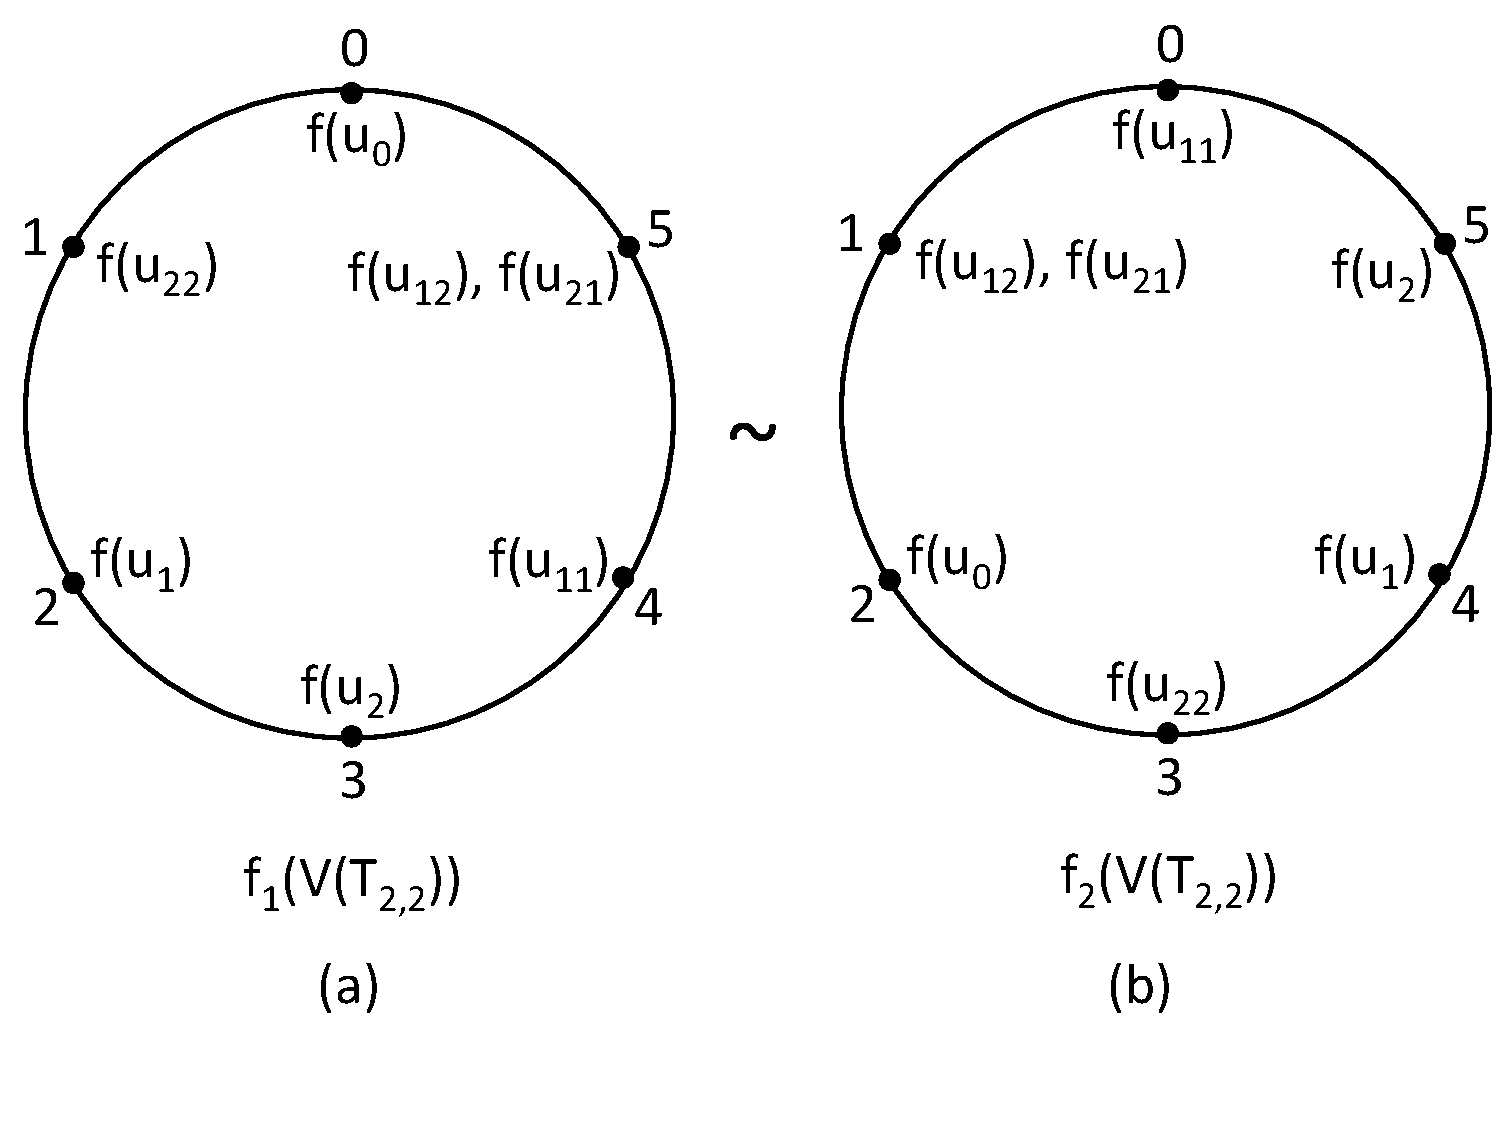
\includegraphics[scale=0.4]{../figures/fig4-3.pdf} 
    \vspace{-10pt}
\caption{Equivalent relation between two $C(h,1,1)$-labellings of a $T_{2,2}$}
\label{fig equivalent}
\end{figure} 
\end{example}

\begin{remark}
\label{rmk:fix0}
From now on, we assume without loss of generality that if $f$ is a $C(h,p,q)$-labelling of a tree $T$, then the root of $T$ is always assigned the label $0$. Since if it does not, then we can rotate $C^n$ to make sure the root of $T$ obtaining $0$. The rotation is well-defined according to Definition \ref{def:equi}.
\end{remark}


%\begin{proposition}
%Let $T$ and $H$ be defined as above. Let $f_{1}$ and $f_{2}$ be two $C_{h,1,1}$-labelling functions, which takes vertices $u$ and $v$ as the first vertex maps to the cycle $H$ respectively. Then, we have $f_{1} \sim f_{2}$.  
%\end{proposition}






%%%%%%%%%%%%%%%%%%%%%%%%%%%%%%%%%%%%
\section{Known results for cyclic metric labelling problem} 
As the cyclic metric labelling problem is not as widely studied as the linear metric labelling problem, we will only review this problem for outerplanar graphs. 
\subsection{Outerplanar graphs}

In section \ref{linear outerplanar}, we mentioned that \cite{bodlaender04} conjectured the minimum span of the $L(2,1)$-labelling of outerplanar graphs $G$ is bounded above by $\Delta+2$. Motivated by this conjecture, \cite{liu05} proved results for cyclic metric labelling of outerplanar graphs $G$ under distance two constraints. In particular, they proved \citeauthor{bodlaender04}'s conjecture to be true, but only for outerplanar graphs with large maximum degree. The authors first proved a connection between the minimum span of the $L(2,1)$ and $C(2,1)$-labelling of outerplanar graphs; i.e.,  
\begin{align}
\label{relation1}
\lambda_{2,1}(G) \le \t_{2,1}(G) \le \lambda_{2,1}(G) +2.
\end{align}
Then they proved that for any outerplanar graph $G$ with the maximum degree $\Delta(G) \ge 15$, the minimum span of $C(2,1)$-labelling is $\t_{2,1}(G) = \Delta+3$. By this result and \eqref{relation1}, \citeauthor{bodlaender04}'s conjecture is proved, but only for $G$ with large maximum degree. They also proved the following.
\begin{theorem}
For any outerplanar graph $G$, the minimum span  $\t_{2,1}(G) \le \Delta+7$. Moreover, if $G$ is triangulated then $\t_{2,1}(G) \le \Delta +5$. 
\end{theorem}
\begin{theorem}
If $G$ is an outerplanar graph and $\Delta \ge 11$ then $\t_{2,1}(G) \le \Delta + 4$. 
\end{theorem}

For outerplanar graph $G$ with small maximum degree. ($\Delta \in [2,5]$) \cite{liu05} proved that the minimum span $\t_{2,1}(G) = \Delta+ 4$.

In the next section, we will present to the reader our results of $C(h,1,1)$-labelling of complete $m$-ary trees. 

%%%%%%%%%%%%%%%%%%%%%%%%
\section{The $C(h,1,1)$-labelling problem}
\label{sec:cyc}
Our results are separated into two parts based on the height of a complete $m$-ary tree. The first part deals with the problem of complete $m$-ary trees $\tmk$ with height $k=2$, while the second part deals with the case when $k \ge 3$. 


%%%%%%%%%%%%%%%%%%%%%%%%%%%%%%%%%%%%

\subsection{Complete $m$-ary tree with height $2$}
Recall that we only deal with the $\lhpq$ and $\chpq$-labelling problems for $h \ge 2$. This assumption is used throughout this thesis.
\begin{remark}
For a complete $m$-ary tree $\tmk$ with $k \ge 2$, the $C(1,1,1)$-labelling problem is the same as the $L(1,1,1)$-labelling problem. In other words, we have $\t_{1,1,1}(\tmk) = \lambda_{1,1,1}(\tmk)$, for $k \ge 2$. 
\end{remark}

The next theorem is the major result for the $C(h,1,1)$-labelling problem of $\tm2$. It also indicates the connection of the minimum spans of these two labellings. 
\begin{theorem}
\label{thm:ck2}
For a complete $m$-ary tree $\tm2$, the minimum span of the $C(h,1,1)$-labelling is  
\begin{align}
\label{ck2}
\t_{h,1,1}(\tm2) &= \max\{\lamh11(\tm2), \lamh11(\tm2)+h-m\}\\
\label{ck22}
&= \max\{2m+h-1, 2h+m-1\}.
\end{align}
\end{theorem}

\eqref{ck22} is a consequence of \eqref{ck2} provided Theorem \ref{thm:h11} is known. The value $2m+h-1$ is achieved for $h\le m$, while $2h+m-1$ is achieved for $h \ge m$. 
\\
\begin{proof} The first step is to prove the minimum span $\t_{h,1,1}(\tm2) \ge  \max\{2m+h-1, 2h+m-1\}$. By Corollary \ref{cor:compare}, we have $\lambda_{h,1,1}(\tm2) \le \t_{h,1,1}(\tm2)$. It follows that $\t_{h,1,1}(T) \ge 2m+h-1$. 

To complete the first step, we need to show the minimum span also satisfies $\t_{h,1,1}(\tm2) \ge 2h+m-1$. This can be proved by contradiction. Assume $\th11(\tm2) \le 2h+m-2$. Then there exists a $C(h,1,1)$-labelling 
\[
f:V(\tm2) \rightarrow V(C^n)
\]
from vertices of height $2$ complete $m$-ary trees to a labelled $n$-cycle, such that $span(f) = 2h+m-2$. By Remark \ref{rmk:fix0}, the root $u_0$ bears the label $0$. As $u_i \in C(u_0)$, for the function $f$ to be a $C(h,1,1)$-labelling of $\tm2$, we must have $f(C(u_0))=\{f(u_{i}) \mid i \in [1,m]\} \subseteq [h, h+m-1]$. Since the cardinality of the set $[h, h+m-1]$ is $m$, it follows $\{f(u_{i}) \mid i \in [1,m]\} = [h, h+m-1]$. Without loss of generality, assume $f(u_i) = h+i-1$. Then we have $f(u_1) = h$ and $f(C(u_1)) \subseteq [2h, 2h+m-2]$, see Fig. \ref{4.3}. There are only $m-1$ labels in the set $[2h, 2h+m-2]$, while the cardinality of $C(u_1)$ is $m$ and each vertex requires a distinctive label. Hence, the assumption $span(f) = 2h+m-2$ is not sufficient to $C(h,1,1)$-label $\tm2$. Therefore, we must have $\t_{h,1,1}(\tm2) \ge 2h+m-1$ when $h \ge m$.
\begin{figure}
  \centering
     \vspace{-0pt}
    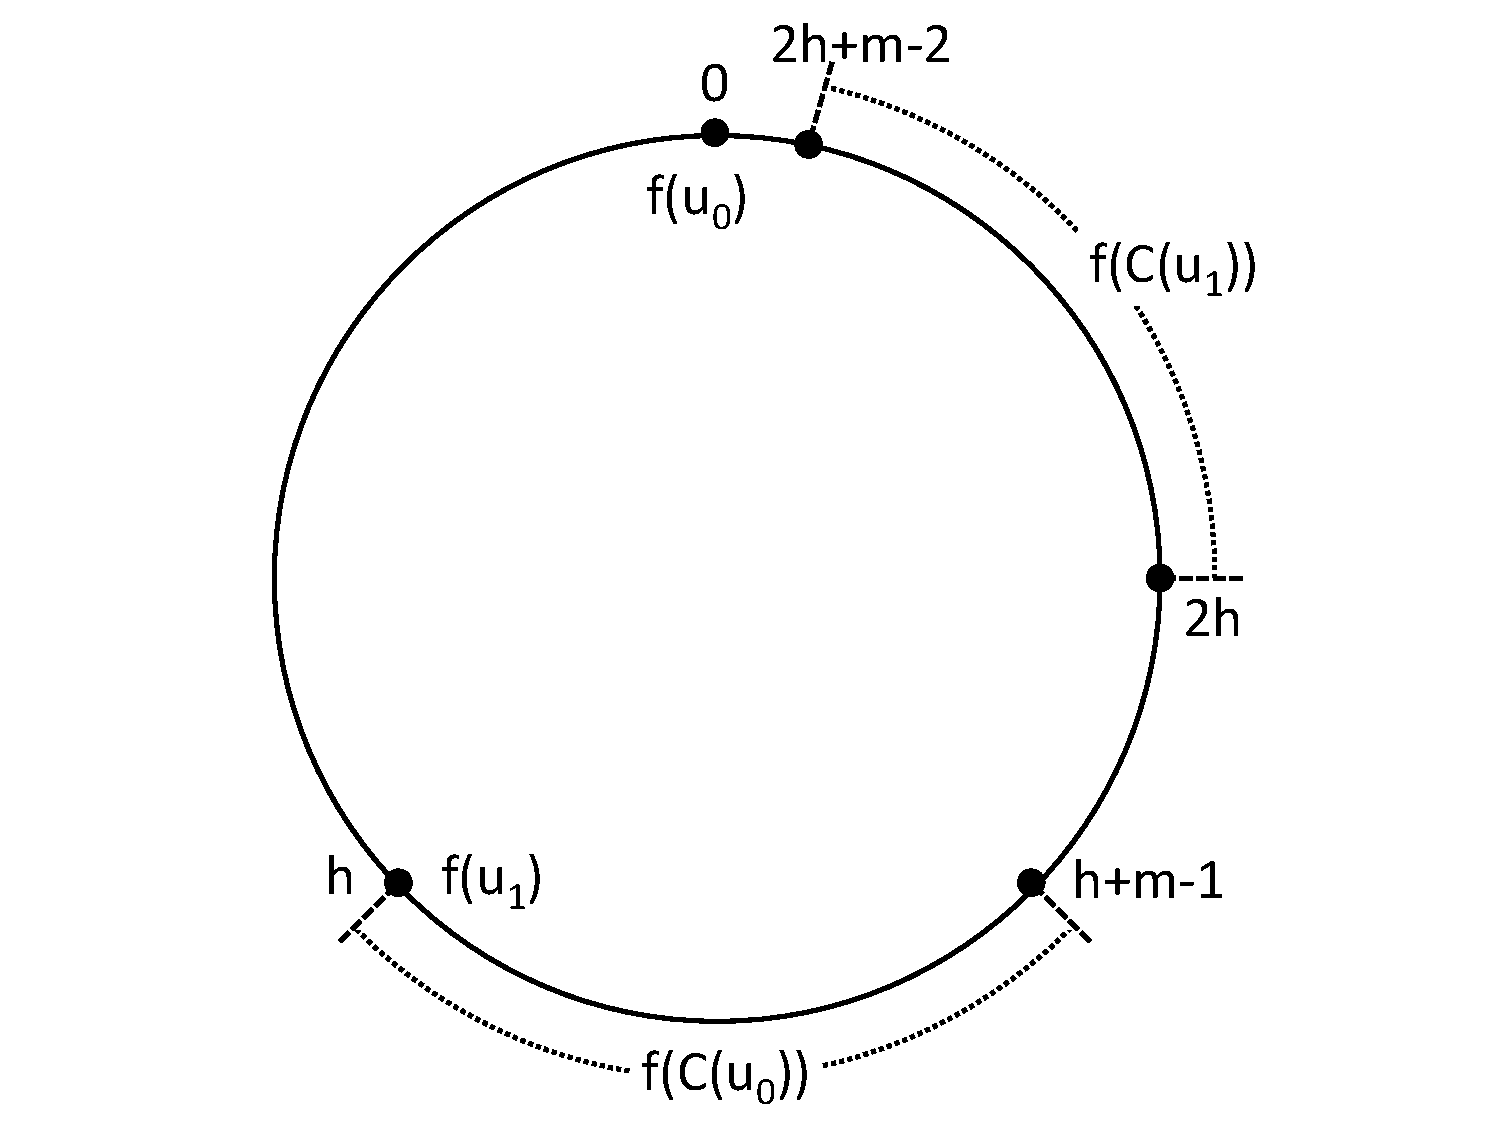
\includegraphics[scale=0.35]{../figures/fig4-4.pdf}
    \vspace{-0pt}
\caption{$span(f) = 2h+m-2$ is not sufficient to $C(h,1,1)$-label $\tm2$}
\label{4.3}
\end{figure}

So far we have proved that $\t_{h,1,1}(\tm2) \ge  \max\{2m+h-1, 2h+m-1\}$. It remains to show that $\t_{h,1,1}(T) \le \max\{2m+h-1, 2h+m-1\}$. If we can find a function $f : V(\tm2) \rightarrow V(C^n)$ with $span(f) = \max\{2m+h-1, 2h+m-1\}$, then we are done. 

Notice that the function $f$ varies for different values of $h$ and $m$. If $h \le m$, then $f$ labels $\tm2$ as follows: 
\begin{enumerate}[(1)]
\item $f(u_0) = 0$;
\item $\{f(u_i) \mid i \in [1,m]\} = [h,h+m-1]$ such that $f(u_i) = h+i-1$;
\item If $i \in [1, m-h+1]$, then $f(C(u_i)) = [h+m, 2m+h-1]$; \\if $i \in [m-h+2, m]$, then $f(C(u_i)) = [2h+i-1, m+2h+i-1] \setminus \{0\}  \pmod {2m+h}$.
\end{enumerate}
On the other hand, if $h \ge m$, then the function $f$ is defined as follows: 
\begin{enumerate}[(1)]
\item $f(u_0) = 0$;
\item $\{f(u_i) \mid i \in [1,m]\} = [h,h+m-1]$ such that $f(u_i) = h+i-1$;
\item $f(C(u_i)) = [2h+i-1, 2h+m+i-1] \setminus \{0\} \pmod {2h+m}$.
\end{enumerate}

It is not hard to check that the function $f$ defined above indeed is a $C(h,1,1)$-labelling of $\tm2$ with $span(f) = \max\{2m+h-1, 2h+m-1\}$. Moreover, the two cases of $f$ are identical when $h = m$. 
\end{proof}
\qed


%%%%%%%%%%%%%%%%%%%%%%
\subsection{Complete $m$-ary trees with height no less than $3$}
\begin{theorem}
\label{thm:ck3}
For a complete $m$-ary tree $\tmk$ with height $k \ge 3$, the minimum span of the $C(h,1,1)$-labelling is \begin{align}
\t_{h,1,1}(T) & = \max\{\lambda_{h,1,1}(\tmk), \lambda_{h,1,1}(\tmk)+h-m-1\} \\
\label{eq:bd1}
&= \max\{2m+h, 2h+m-1\}.
\end{align}
\end{theorem}

Similarly, $\lambda_{h,1,1}(\tmk)$ achieves $2m+h$ when $h \le m+1$, $2h+m-1$ when $h \ge m+1$. 

\begin{proof}
The same method is used to prove this theorem. That is, by showing the lower and upper bounds of the minimum span $\t_{h,1,1}(T)$ are identical.   

Corollary \ref{cor:compare} implies $\t_{h,1,1}(\tmk) \ge \lambda_{h,1,1}(\tmk) = 2m+h$ for $k \ge 3$. We also need to show $\t_{h,1,1}(\tmk) \ge 2h+m-1$. According to Theorem \ref{thm:ck2}, the minimum span $\t_{h,1,1}(\tm2) = 2h+m-1$ for $h \ge m$. Hence, it is obvious that the minimum span will be no less than $2h+m-1$ for larger complete $m$-ary trees $\tmk$ with $k \ge 3$. Precisely, $\t_{h,1,1}(\tmk) \ge 2h+m-1$ for $k \ge 3$.   

The trick of the proof is to find a function $$f:V(\tmk) \rightarrow V(C^n)$$ such that a complete $m$-ary tree $\tmk$ with $k \ge 3$ is $C(h,1,1)$-labelled by $f$ with
\[
span(f) =  \max\{2m+h, 2h+m-1\}.
\]
Lemma \ref{lem:consecutive} below proves the existence of such a function. 
\end{proof}
\qed

We are dealing with all complete $m$-ary trees $\tmk$ with $k \ge 3$. Hence, the height of such a tree could be infinite. The objective of this problem is to map vertices of $\tmk$ to vertices on a labelled $n$-cycle with $n$ as small as possible. 

For the cyclic metric, when mapping vertices of $\tmk$ to vertices on a cycle, the mapping can go around the cycle again and again. Hence the degree of difficulty involved in establishing a pattern is increase.  

Nevertheless, the essential observation is that the neighbours of every internal vertex can be mapped to a consecutive set of vertices on $C^n$. The following lemma states this observation explicitly, but in a slightly different family of trees

In Definition \ref{neighbour}, we defined the neighbours of a vertex $u \in V(G)$ in graph $G$ to be the set of vertices adjacent to $u$; i.e.,  $N(u) := \{v \in V(G) \mid d(u,v) = 1\}$. We define another notation $\overline{N(u)} :=\{u\} \cup N(u)$.

\begin{lemma}
\label{lem:consecutive}
Let $\tilde{T}$ be a complete $m$-ary tree with an extra edge attached to the root of it; i.e.,  $\tilde{T} := \tmk +\{u_0v\}$, where $v$ is the root $\tmk$. Then, there is a $C(h,1,1)$-labelling $f: V(\tilde{T}) \rightarrow V(C^n)$ such that 
\begin{enumerate}[(1)] 
\item $span(f) = \max\{2m+h, 2h+m-1\}$;
\item for any vertex $u \in V(\tilde{T})$ with $d(u) = m+1$, its neighbours $N(u)$ can be labelled consecutively by the map $f$ for all values of $h$ and $m$.   
\end{enumerate}
\end{lemma}   

The way we construct $\tilde{T}$ means that every complete $m$-ary tree $\tmk$ is covered by a $\tilde{T}$. Accordingly, if the lemma holds for $\tilde{T}$, then it also holds for $\tmk$. 
\\
\begin{proof}
The first step is to use induction to show $(2)$, provided $\max\{V(C^n)\} = \t_{h,1,1}(\tilde{T})$. The following are the two inductive steps: 
\begin{enumerate}[(i)]
\item for the root $u_0$ of $\tilde{T}$, $f(N(u_0))$ is a consecutive set of labels.
\item for any vertex $u_{0\dots jk} \in V(\tilde{T})$ with $d(u_{0\dots jk}) = m+1$, if $u_{0\dots jk}$ and $N(u_{0\dots jk})$ have been labelled, and $f(N(u_{0\dots jk}))$ is assigned a consecutive label set, then $f(N(u_{0\dots jkl}))$ can also be assigned a consecutive label set, for any vertex $u_{0\dots jkl} \in C(u_{0\dots jk})$ with $d(u_{0\dots jkl}) = m+1$. 
\end{enumerate} 

Without loss of generality, assume label $u_0$ and its neighbours $N(u_0)$ first. In this case, $f(N(u_0))$  is a consecutive part on $C^n$. Then step (i) is trivial. 

To prove step (ii), we note that if the function $f$ is a $C(h,1,1)$-labelling of $\tilde{T}$, then it needs to satisfy the following condition when labelling $C(u_{0\dots jkl})$:  
\begin{align}
\label{condition1}
&f(C(u_{0\dots jkl})) \subseteq V(C^n) \setminus (S \cup W)
\end{align}  
where 
\begin{align*}
S &:= f(\overline{N(u_{0\dots jk})}) \\
W &:= [f(u_{0\dots jkl}) - (h-1), f(u_{0\dots jkl}) + (h-1)].
\end{align*}

The cardinality $|S| = m+2$ by definition. Moreover, by assumption in (ii) we have $f(N(u_{0\dots jk}))$ is consecutive. Thus the set $S$ consists of one consecutive segment and one single label with a separation at least $h$. The way $W$ is defined ensures that it is consecutive with cardinality $|W| = 2h-1$. Moreover, $S \cap W \neq \emptyset$, since $u_{0\dots jkl} \in N(u_{0\dots jk})$. This implies $Q:=f(N(u_{0 \dots jk})) \cup W$ is still a consecutive segment of larger cardinality. Notice that $f(u_{0\dots jk}) \not\in Q$, as it has separation at least $h$ with $f(N(u_{0\dots jk}))$. But it can be adjacent $Q$. Hence $S\cup W$ is either a consecutive set or a consecutive set union single label. Equivalently, $V(C^n) \setminus (S \cup W)$ consists of either one consecutive set or two consecutive sets separated by $f(u_{0\dots jk}) \cup Q$ (Fig. \ref{lemma ex 1}, Fig. \ref{lemma ex 11}).

\begin{figure}
 \centering
     \vspace{-0pt}
    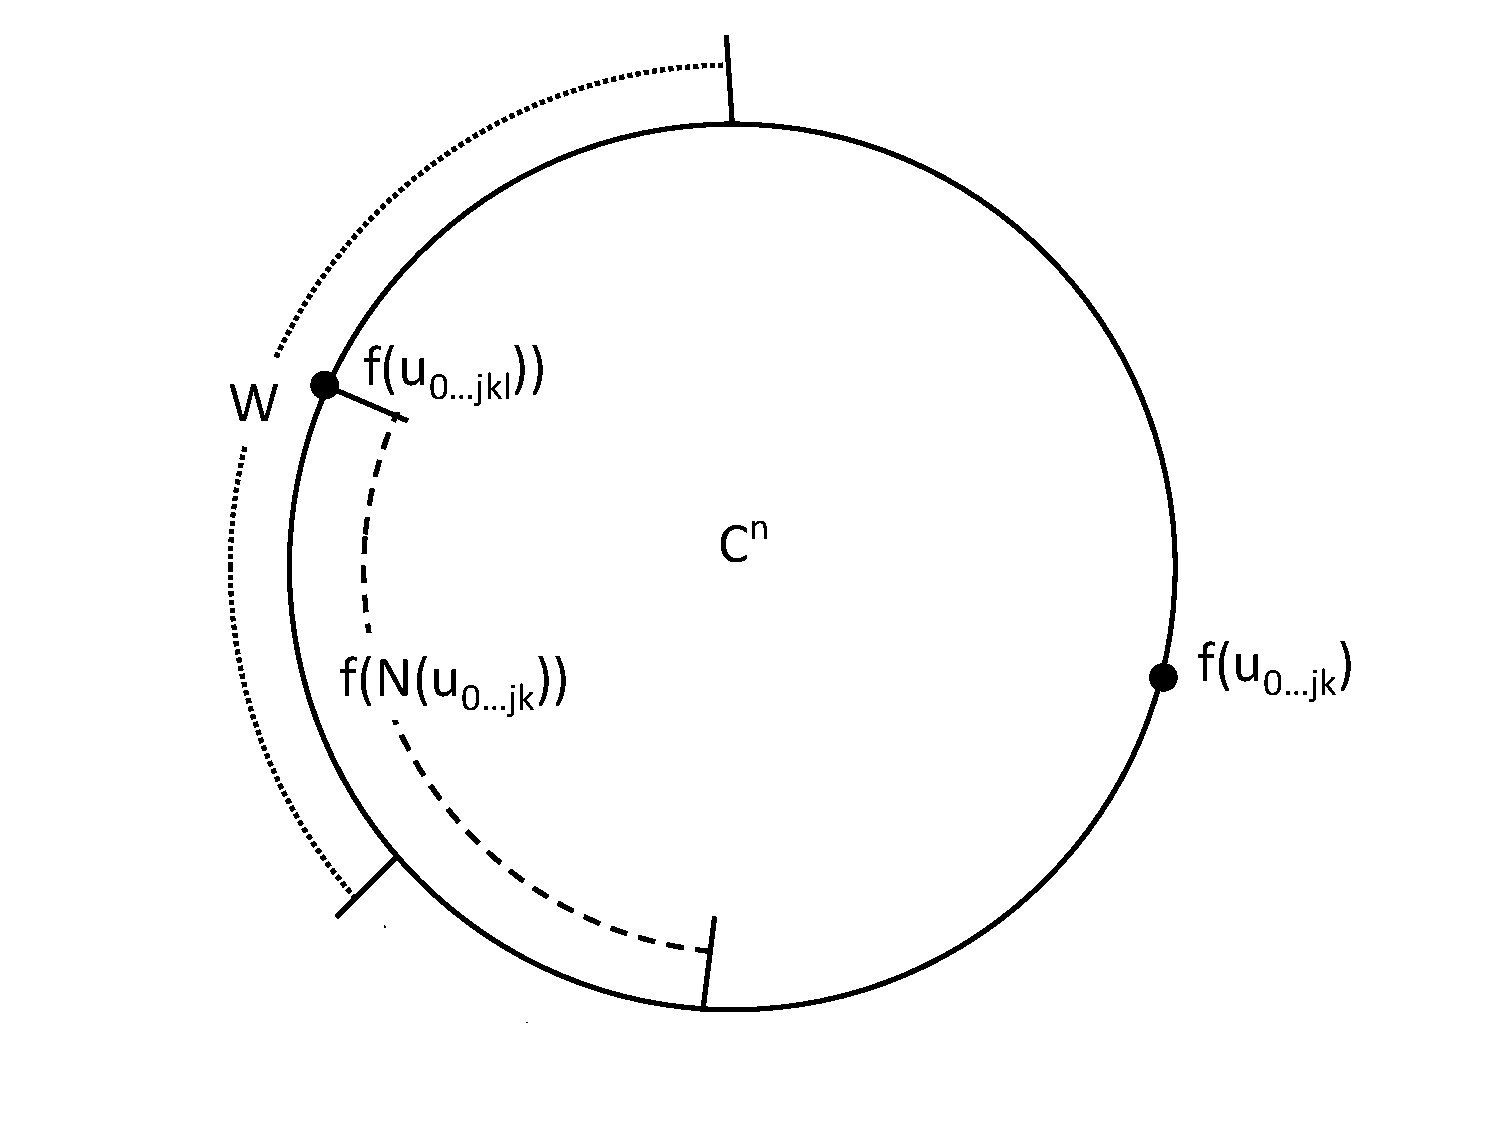
\includegraphics[scale=0.45]{../figures/fig4-5-a.pdf}
   \vspace{-0pt}
\caption{Two consecutive sets for $C(u_{0\dots jkl})$} 
\label{lemma ex 1}
\end{figure}

\begin{figure}
 \centering
     \vspace{-0pt}
    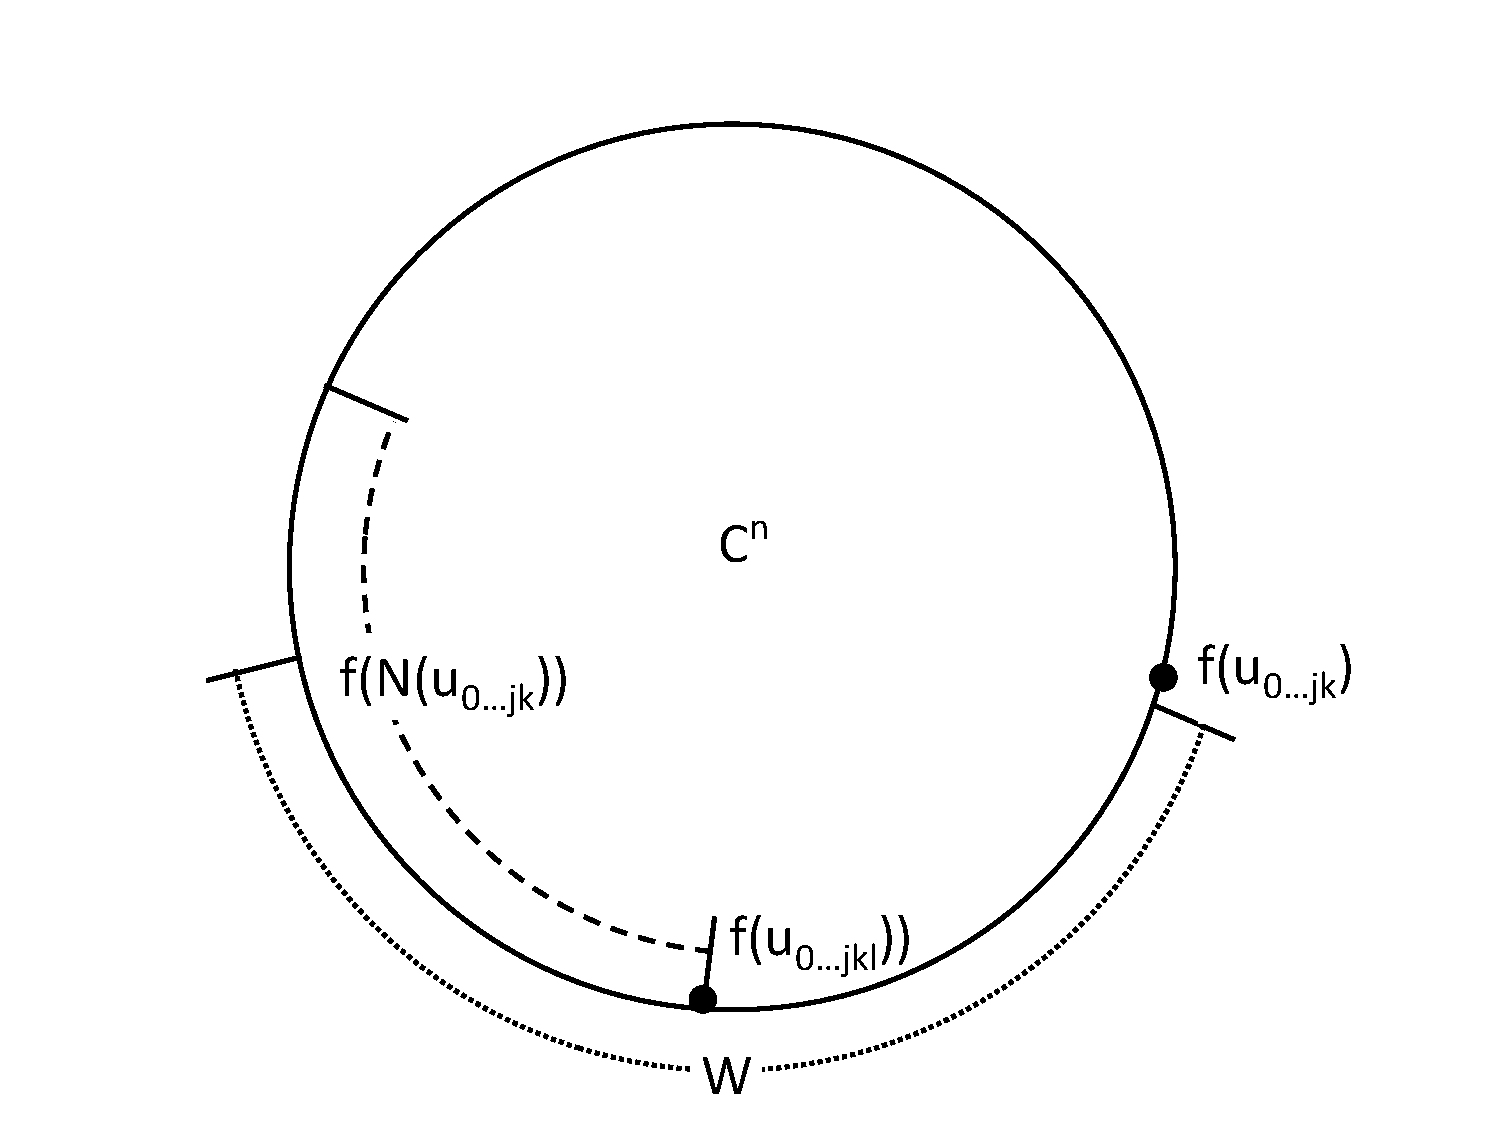
\includegraphics[scale=0.45]{../figures/fig4-5-b.pdf}
   \vspace{-0pt}
\caption{One consecutive set for $C(u_{0\dots jkl})$} 
\label{lemma ex 11}
\end{figure}
 

Use $(S \cup W)^c$ to denote $V(C^n) \setminus (S \cup W)$ now. Since $u_{0\dots jk} \in N(u_{0\dots jkl})$, then 
\begin{align}
\label{equ:condition2}
f(N(u_{0\dots jkl})) \subseteq (S \cup W)^c \cup \{f(u_{0\dots jk})\}.
\end{align}

\eqref{equ:condition2} implies that in either case $f(N(u_{0\dots jkl}))$ is a consecutive set. Thus (ii) is proved.

In fact, it is not hard to see that the cardinality of the set $Q$ is dependent upon the position of $u_{0\dots jkl}$ in $N(u_{0\dots jk})$. In particular, it obtains the largest cardinality when $u_{0\dots jkl}$ is one of the end points of $N(u_{0\dots jk})$. Equivalently, $S \cup W$ reaches its maximum size when the intersection $S\cap W$ has the smallest cardinality, as $|S \cup W| = |S| + |W| - |S \cap W|$. Thus to compute the cardinality of $S\cup W$, we consider the following two cases. 

If $h < m$, then $\min\{|S \cap W|\} = h$. This occurs when $u_{0\dots jkl}$ is one of the end points of $N(u_{0\dots jk})$. Thus we have 
\begin{align*}
|S \cup W| &= |S| + |W| - |S \cap W| \\
& \le |S| + |W| - \min\{|S \cup W|\} \\
& = (m+2) + (2h-1) - h\\
&= m+h+1.
\end{align*}

Since $\tau_{h,1,1}(\tilde{T}) = 2m+h$ when $h < m$, then $|V(C^n)| = 2m+h+1$. Thus we have 
\begin{align*}
|V(C^n) \setminus (S \cup W)| &= |V(C^n)| - |S\cup W|\\
& \ge (2m+h+1) - (m+h+1) \\
&= m.
\end{align*}
This shows that there are just enough labels for the function $f$ to $C(h,1,1)$-label $C(u_{0\dots jkl})$, as $|C(u_{0\dots jkl})| = m$. 

If $h \ge m$, the situation is easier, because the set $f(N(u_{0\dots jk})) \subsetneq W$ is contained in $W$ as a subset, no matter where $u_{0\dots jkl}$ is located in the set $N(u_{0\dots jk})$ (Fig. \ref{lemma ex 2}). Hence, $|S \cup W| = |W| +1= 2h$. This implies 
\begin{align*}
 |V(C^n) \setminus (S \cup W)| &=
 \begin{cases}
 (2m+h+1) -2h & \text{ if } h =m,\\
 (2h+m)-2h & \text{ if } h \ge m+1.
 \end{cases}\\
&=  \begin{cases}
   m+1 & \text{if } h = m,\\
   m       & \text{if } h \ge  m+1.
  \end{cases}
\end{align*}
This also shows there are enough labels for the function $f$ to $C(h,1,1)$-label $C(u_{0\dots jkl})$. This completes the proof.  
\end{proof}
\qed
\begin{figure}
 \centering
     \vspace{-10pt}
    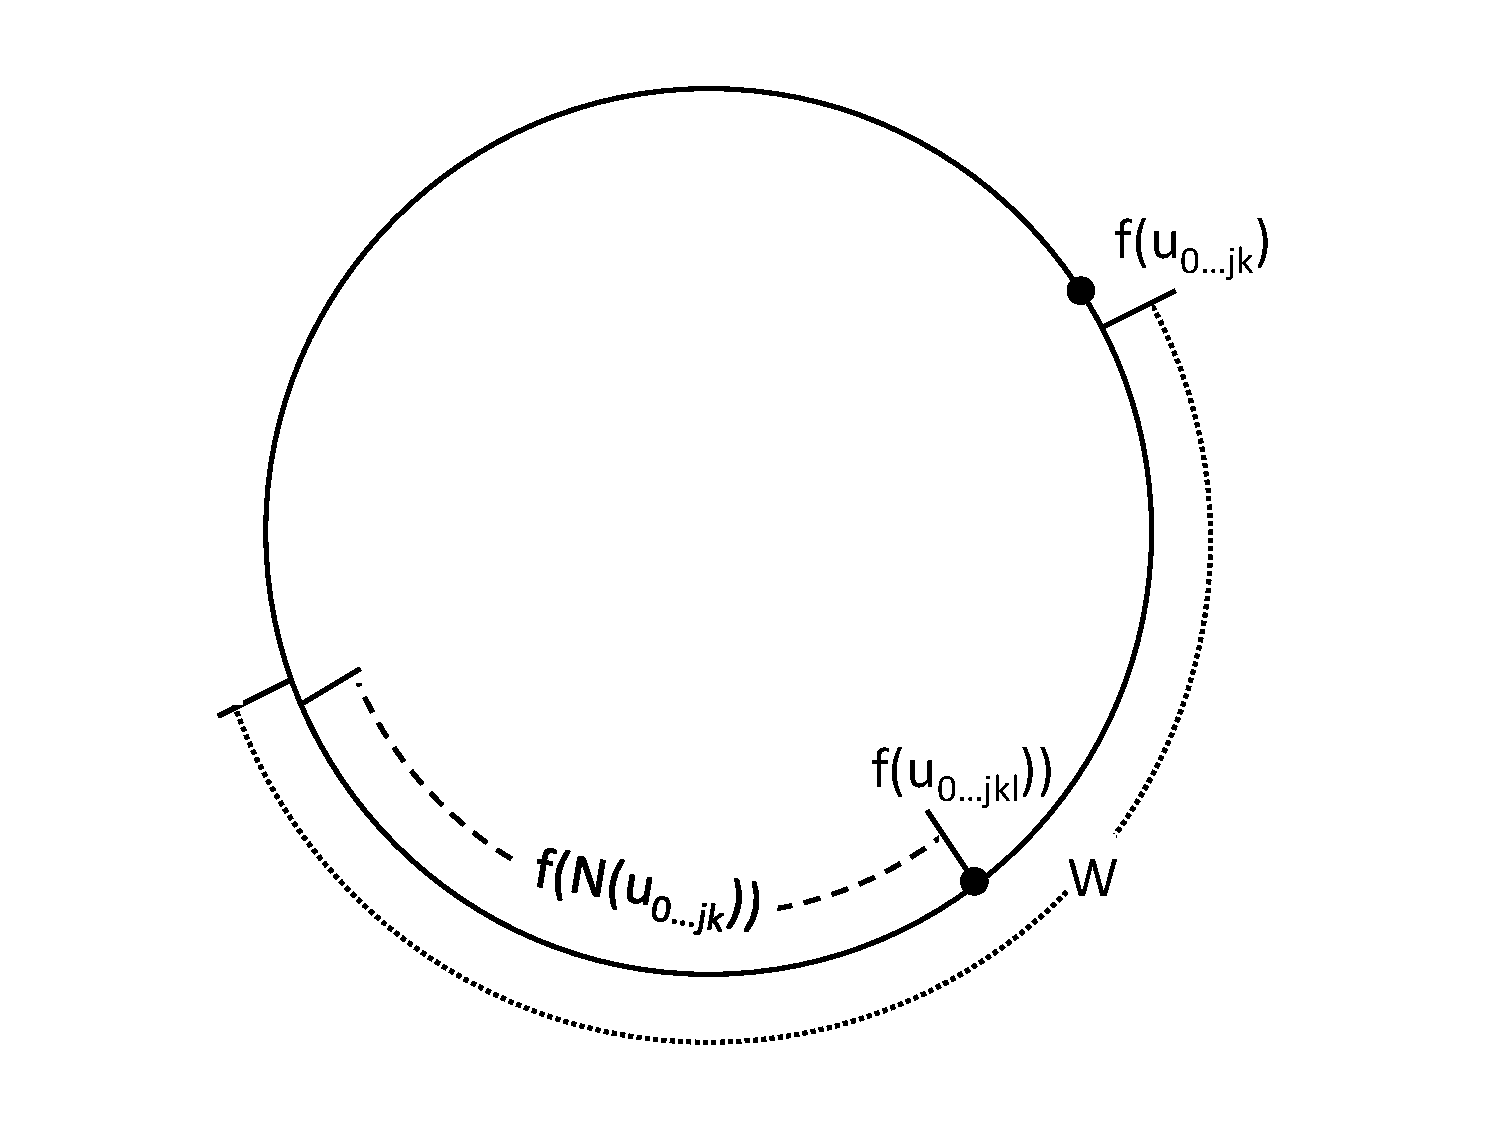
\includegraphics[scale=0.4]{../figures/fig4-7.pdf}
    \vspace{-0pt}
\caption{Special case when $f(N(u_{0\dots jk})) \subsetneq W$} 
\label{lemma ex 2}
\end{figure}


If we apply this lemma to complete $m$-ary trees $\tmk$ with height $k \ge 3$, then obviously it ensures the existence of a function $f$, which $C(h,1,1)$-labels $\tmk$ with the minimum span $\t_{h,1,1}(\tmk) = \max\{2m+h, 2h+m-1\}$ for $k \ge 3$. Thus Theorem \ref{thm:ck3} is proved. 

\begin{remark}
\label{howtolabel}
Lemma \ref{lem:consecutive} in fact gives an almost explicit way of how to label vertices of a complete $m$-ary tree $\tmk$ for $k \ge 3$. In the proof we see that \eqref{condition1} gives an exact label set for $C(u_{0\dots jkl})$ when $h<m$, while it provides $1$ extra label when $h \ge m+1$ and $2$ extra labels when $h=m$. 
\end{remark}

In this section, we solved the $C(h,1,1)$-labelling problem of complete $m$-ary trees. We proved that the minimum span $\t_{h,1,1}(\tm2)$ and $\t_{h,1,1}(\tmk)$ for $k \ge 3$ can be solved exactly, but dependent upon the values of $h$ and $m$. In the next section, we are aiming for generalising these results to $\chpq$-labelling problems of complete $m$-ary trees. 

%%%%%%%%%%%%%%%%%%%%%%%%%%%%%%%%%%%%
\section{The $C(h,p, q)$-labelling problem}

In this section, we extend our previous study of the cyclic metric labelling problem to a more general version, the $C(h,p,q)$-labelling problem, where $h \ge p \ge q \ge 1$. The set of trees we will deal with in this section is still the set of complete $m$-ary trees. 


%%%%%%%%%%%%%%%%%%%%%%%%%%%%%%%%%%%%


\subsection{Complete $m$-ary tree $\tm2$ with height $2$}
\begin{theorem}
\label{chpq2}
For a complete $m$-ary tree $\tm2$, if $h \ge (m-1)p+q$, then the minimum span of the $\chpq$-labelling is 
\begin{align*}
\thpq(\tm2)= 2h+mp-1. 
\end{align*}
\end{theorem}

When substituting $p=q=1$ into this theorem, the result is the same as Theorem \ref{thm:ck2} claims for $h \ge m$. 
\\
\begin{proof}
We first prove by contradiction that $2h+mp-1$ is the lower bound of $\thpq(\tm2)$. Suppose the minimum span $\thpq(\tm2) \le 2h+mp-2$. Then there exists a map $f:V(\tm2) \rightarrow V(C^n)$ such that $f$ is a $\chpq$-labelling of $\tm2$ with $span(f) = 2h+mp-2$. 

Without loss of generality, assume $f$ labels some vertices of $\tm2$ as follows: 

\begin{enumerate}[(1)]
\item $f(u_0) = 0$;
\item $\{f(u_i) \mid i \in [1,m]\} = h+[0,m-1]p$ such that $f(u_i) = h+(i-1)p$.
\end{enumerate}
In particular, $f(u_1) = h$. Since $h \ge (m-1)p+q$, then $2h \ge h+(m-1)p+q$. This implies the minimum available label for $C(u_1)$ is $2h$. Since the cardinality $|C(u_1)| = m$, then $\max(f(C(u_1))) = 2h+(m-1)p$. However, since $span(f) =2h+mp-2$, then $|f(u_0) - \max(f(C(u_1)))| = p-1$.This is a contradiction, as $d(u_0, v) = 2$ for all $v \in C(u_1)$. 

So far, we have showed that $\thpq(\tm2) \ge 2h+mp-1$. It remains to show that $\thpq(\tm2) \le 2h+mp-1$. 

We define a function $f: V(\tm2) \rightarrow V(C^n)$ from vertices of $\tm2$ to vertices of a labelled $n$-cycle as follows: 
\begin{enumerate}[(1)]
\item same as (1) above;
\item same as (2) above. 
\end{enumerate}
For the children set $C(u_i)$, we can use labels from the set $[0,f(u_i) - h]$ and $[f(u_i)+h, f(u_0) - p]$. We assumed $h \ge (m-1)p+q$, then the $p$-consecutive label set $[0,m-1]p \subset [0, h]$ is available to $C(u_i)$. By step (2), we  have $\{r_1p \mid 1 \le r_1 \le \min\{i-1, m-1\}\}\subset f(C(u_i))$. As $i \in [1,m]$, then $\min\{i-1,m-1\}=i-1$. It is equivalent to say $\{r_1p \mid 1 \le r_1 \le i-1\} \subset f(C(u_i))$. We have assigned $(i-1)$ labels to vertices in the set $C(u_i)$, there are $(m-i+1)$ vertices remaining. We need to use labels from the set $[f(u_i)+h, f(u_0) - p]$ for those remaining vertices. Then we have $\{f(u_i) + h + r_2p \mid 0 \le r_2 \le m-1-r_1\} = \{2h+(i+r_2-1)p \mid 0 \le r_2 \le m-i\} \subset f(C(u_i))$. Hence, we construct the last step as 
\begin{enumerate}[(3)]
\item $f(u_{ij}) = \{2h+(i+r_2-1)p \mid r_2 \in [0,m-i]\} \cup \{r_1p \mid r_1 \in [1,i-1]\}$. 
\end{enumerate}

From (3), we can see $\max(f(C(u_i))) = 2h+(m-1)p$. Then $span(f) = 2h+mp-1$. This implies $\thpq(\tm2) \le 2h+mp-1$. 
\end{proof}
\qed


\begin{theorem}
\label{thm:chpq2}
Let $n := \max\{r \in [1,m-1] \mid rp \le h\}$. Define the following two conditions 
\begin{enumerate}[(i)]
\item $h-np < q$;
\item $p < 2q$.	
\end{enumerate}
If $h \le (m-1)p+q$, then the minimum span of the $\chpq$-labelling of any complete $m$-ary tree $\tm2$ is 
\begin{align*}
\thpq(\tm2)= 
 \begin{cases}
 2h+(2m-n)p-1 & \text{ if } (i) \text{ and } (ii) \text{ are true}, \\
 2h+(2m-n-1)p-1 & \text{ if } (i) \text{ is false but } (ii) \text{ is true}, \\
 2h+(m+1)p-1 & \text{ if } (i) \text{ is true but } (i) \text{ is false}, \\
 2h+mp-1 & \text{ if } (i) \text{ and } (ii) \text{ are false}\\ &\text{ and } (n+1)p-h \ge q, \\
 2h+(m+1)p-1 & \text{ if } (i) \text{ and } (ii) \text{ are false}\\ &\text{ and } (n+1)p-h < q.
 \end{cases}
\end{align*}
\end{theorem}

Notice that if $p = q = 1$, then $h \le (m-1)p+q$ implies $h \le m$. Thus we have $n = \min\{h, m-1\}$. Also, if $p=q=1$, then (ii) is true. But (i) is true only when $h \le m-1$, while it is false when $h > m-1$; i.e.,  when $h = m$. Thus, we have $\thpq(\tm2) = 2h+(2m-n)-1$ for $h \le m-1$ and $\thpq(\tm2) = 2h+(2m-n-1)-1$ for $h = m$. In the end, we get the minimum span $\thpq(\tm2) = 2m+h-1$ for $ h \le m$. This is the same as the result in Theorem \ref{thm:ck2} for $h \le m$.

Also notice that if $h = (m-1)p+q$, then $n = m-1$. This implies (i) is false, but tells nothing about (ii). If (ii) is true then $\thpq(\tm2) = 2h+(2m-n-1)p-1 = 2h+(2m-m+1-1)p-1=2h+mp-1$. If (ii) is false, then it follows $(n+1)p - h \ge q$, so $\thpq(\tm2) = 2h+mp-1$. Both of these two cases give the same $\thpq$ value as that in Theorem \ref{chpq2} when $h = (m-1)p+q$. 
\\
\begin{proof}
First, we prove the above values are lower bounds for $\thpq(\tm2)$ in each case. Without loss of generality, in all cases we use the same labels for $u_0$ and $C(u_0)$ as before. That is,  

\begin{enumerate}[(1)]
\item $f(u_0) = 0$;
\item $\{f(u_i) \mid i \in [1,m]\} = h + [0,m-1]p$ such that $f(u_i) = h + (i-1)p$. 
\end{enumerate}
But the children $C(u_i)$ are labelled differently for $i \in [1,m]$. To prove by contradiction, in each case we will assume $\thpq(\tm2) \le b$, where $b+1$ equals what this theorem claims. Hence, there must exist a $\chpq$-labelling function $f:V(\tm2) \rightarrow V(C^n)$ such that $span(f) = b$.  

If (i) and (ii) are both true, then $span(f)= 2h+(2m-n)p-2$. By (2) we have $f(u_m) = h+(m-1)p$. Condition (i) implies  $\{f(u_{mj}) \mid j \in [1,n-1]\}=[1,n-1]p$. Condition (ii) implies $\{f(u_{mj}) \mid j \in [n, m]\} =2h+(m-1)p+[0,m-n]p$. Then we have $\max(f(C(u_m)))= 2h+(2m-n-1)p$. Moreover, the distance $d(u_0, u_{mm}) = 2$ implies $|f(u_0)-f(u_{mi})| \ge p$ for all $i \in [1,m]$. But $|f(u_0) - \max(f(C(u_m)))| =p-1$ contradicts this condition. Hence, we must have $\thpq(\tm2) \ge 2h+(2m-n)p-1$. 

If (i) is false but (ii) is true, then $span(f) = 2h+(2m-n-1)p-2$. Similarly, by (2) we have $f(u_m) = h+(m-1)p$. Condition (i) is false implies $\{f(u_{mj}) \mid j \in [1,n]\}=[1,n]p$. Condition (ii) implies $\{f(u_{mj}) \mid j \in [n+1, m]\} = 2h+(m-1)p+[0,m-n-1]p$. By the same argument as above, we have $|f(u_0) - \max(f(C(u_m)))| = p-1$, which is also a contradiction. 

If (i) is true but (ii) is false, then $span(f) = 2h+(m+1)p-2$. By (2) and (i) we have $f(u_m) = h+(m-1)p$, and $\{f(u_{mj}) \mid j \in [1,n-1]\} = [1,n-1]p$. The false of condition (ii) implies there may be some labels in the segment $[f(u_i), f(u_{i+1})]$ that can be used by $f(C(u_m))$. Thus we have $\{f(u_{mj}) \mid j \in [n, m]\} \subset [np, (m-1)p] \cup [2h+(m-1)p, 2h+mp-1]$. Notice that there is only one label available in $[2h+(m-1)p, 2h+mp-1]$; i.e.,  $2h+(m-1)p$. Hence, it remains to find labels from the set $[np, (m-1)p]$ for the rest $(m-n)$ vertices. Condition (i) ensures that $\{np\} \not\in f(C(u_m))$. It follows from this that $[n+1,m-1]p \not\subset f(C(u_m))$. However, since we have (ii) is false, there is an available label between each segment $[ip, (i+1)p]$, where $i \in [n, m-2]$. But there are in total $(m-n-1)$ segments, which implies there are only $(m-n-1)$ labels for the remaining $(m-n)$ vertices. This is a contradiction. 

The last two cases are neither (i) nor (ii) is true. If $(n+1)p-h \ge q$, then assume $span(f) = 2h+mp-2$. We know $f(u_m) = h+(m-1)p$. By (i) is false, we have $\{f(u_{mj}) \mid j \in [1,n]\} = [1,n]p$. By $(n+1)p-h \ge q$ and the false of condition (ii), we get $\{f(u_{mj}) \mid j \in [n+1, m-1]\}=[n+1, m-1]p$. Now, we need one more label for the vertex $u_{mm}$. The minimum available label for $u_{mm}$ is $2h+(m-1)p$. But $|f(u_0) - \min(f(u_{mm}))| = (2h+mp-1)-(2h+(m-1)p) = p-1$ contradicts the fact that $d(u_0, u_{mm}) = 2$. 

On the other hand, if $(n+1)p-h < q$, then $span(f)= 2h+(m+1)p-2$. Again we have $f(u_m) = h+(m-1)p$. The false of condition (i) implies $\{f(u_{mj}) \mid j \in [1,n]\}=[1,n]p$. However, the assumption $(n+1)p-h < q$ implies $[n+1, m-1]p \not\subset f(C(u_m))$. By (ii) is false, there must exist labels in each segment $[i, (i+1)]p$, where $i \in [n+1, m-2]$. Therefore, we have another $(m-n-2)$ labels for vertices in the set $C(u_m)$. So far, we have labelled $(m-2)$ vertices from the set $C(u_m)$. For the remaining two vertices, we let $\{f(u_{mj}) \mid j \in [m-1,m]\} = 2h+(m-1)p+[0,1]p$, which are the minimum available labels for these two vertices. However, there is also a contradiction since $|f(u_0) - \max(f(C(u_m)))| = (2h+(m+1)p-1) - (2h+mp) = p-1$, while $d(u_0, u_{mj}) = 2$ for all $j \in [1,m]$. 

Up to now, we have proved that the values in Theorem \ref{thm:chpq2} are the lower bounds of $\thpq(\tm2)$ in all $5$ cases. It remains to show they are also upper bounds of $\thpq(\tm2)$. This can be verified by constructing a specific labelling in each case. 

We have defined how to label the root $u_0$ and its children $C(u_0)$ by (1) and (2). In the following, we will define how to label $\{C(u_i) \mid i \in [1,m]\}$ in each case.

Whether (i) and (ii) are true in each case imply they bear different label sets. If we can work out the sequential label set in each particular case, then we are done. 

To avoid repeated words, we define the following sets beforehand. If (i) is true, then $[p, (n-1)p] \subseteq f(C(u_i))$. Moreover, we have $|f(u_i) - f(v)| \ge h$ for every $v \in C(u_i)$. Hence we define 
\begin{align*}
L_1 &= \{r_1p \mid p \le r_1p \le \min\{f(u_i)-h, (n-1)p\}\} \\
&=\{r_1p \mid 1 \le r_1 \le \min\{i-1, n-1\}\}.
\end{align*}
If (i) is false, then we have $[p,np] \subseteq f(C(u_i))$. Similar as above, we define 
\begin{align*}
L_1^{c} &= \{r_1p \mid p \le r_1p \le \min\{f(u_i)-h, np\}\}\\
&=\{r_1p \mid 1 \le r_1 \le \min\{i-1, n\}\}.
\end{align*}
If (ii) is true, then there exists no labels in the set $[h, h+(m-1)p]$. Hence we define 
\begin{align*}
L_2 &=\{\max\{f(u_i)+h, f(u_m)+q\} +r_2p \mid 0 \le r_2 \le m-1-|r_1|\}\\ 
&=\{\max\{2h+(i-1)p, h+(m-1)p+q\}+r_2p \mid 0 \le r_2 \le m-1-|r_1|\}.
\end{align*}
Now, suppose (ii) is false, there may exists labels in the set $[h, h+(m-1)p]$. In this case, we define two separated label sets, namely $L_{21}^c$ and $L_{22}^c$, which are contained in the sets $[h, f(u_i)]$ and $[f(u_i), span(f)]$ respectively. If (i) is true, then $\{np\}$ is too close to $f(u_1)$. It follows that $(n+1)p$ is too close to $f(u_2)$, and $(n+2)p$ is too close to $f(u_3)$ etc. In general, $\{np, (n+1)p, (n+2)p, \dots\} \not\subseteq f(C(u_i))$. Since (ii) is false, we can use $\{f(u_1) +q, f(u_2)+q, \dots\}$; i.e., $\{f(u_1)+q, f(u_1)+p+q, \dots\}$. Hence we have 
\[
\{f(u_1)+q +r_2p \mid f(u_1)+q+r_2p \le f(u_i)-h\} \subseteq f(C(u_i)).
\]
From this, we get $\max (r_2)=\lfloor \frac{(i-1)p-h-q}{p}\rfloor$. This implies 
\[
\left\{h+q+r_2p \mid 0 \le r_2 \le \lfloor \frac{(i-1)p-h-q}{p}\rfloor \right\} \subseteq f(C(u_i)).
\]
If (i) is false, then $\{np\} \in f(C(u_i))$. Moreover, if $(n+1)p-h <q$, the case is the same as above. In this case, we use exactly the same set of labels defined above. However, if $(n+1)p \ge q$, then we have 
\[
\{(n+1)p, (n+2)p, \dots \} \subseteq f(C(u_i)).
\]
That is
\[
\{(n+1)p+r_2p \mid (n+1)p+r_2p \le f(u_i)-h\} \subseteq f(C(u_i)).
\]
Thus we get $\max(r_2) = i-n-2$. Then we have 
\[
\{(n+1)p+r_2p \mid 0 \le r_2 \le i-n-2\} \subseteq f(C(u_i)).
\]
Precisely, we label set is 
\begin{align*}
L_{21}^{c} =
\begin{cases}
\left\{h+q+r_2p \mid 0 \le r_2 \le \lfloor \frac{(i-1)p-h-q}{p}\rfloor \right\} \\ \text{ if (i) is true or if } (i) \text{ is false and } (n+1)p-h <q,\\
\{(n+1)p+r_2p \mid 0 \le r_2 \le i-n-2\} \\ \text{ if (i) is false and } (n+1)p-h \ge q,\\
\end{cases}
\end{align*}

For the label set $L_{22}^c$, if $f(u_i)+h \ge f(u_m)$ then the rest of $f(C(u_i))$ belongs to the set $[f(u_m), span(f)]$. As $|f(u_m) -f(v)| \ge q$ for all $v \in C(u_i)$, then we have 
\begin{align*}
\{\max\{f(u_i)+h, f(u_m)+q\} +r_2^*p \mid 0 \le r_2^* \le m-r_1-r_2-1\} \subseteq f(C(u_i))
\end{align*}
If $f(u_j) \le f(u_i)+h \le f(u_{j+1})$ and $f(u_i)+h \le f(u_{j+1})-q$ where $j \in [1,m-1]$, then we have 
\[
\{f(u_{j+1})-q, f(u_{j+2})-q, \dots\} \subseteq f(C(u_i)).
\]
This is equivalent to 
\[
\{f(u_{j+1})-q+r_2^*p \mid 0 \le r_2^* \le m-r_1-r_2-1\} \subseteq f(C(u_i)).
\]
On the other hand, if $f(u_j) \le f(u_i)+h \le f(u_{j+1})$ and \\$f(u_i)+h > f(u_{j+1})-q$, then $\{f(u_{j+1})-q\} \not\in f(C(u_i))$. In this case, we need to take 
\[
\{f(u_{j+1})+q, f(u_{j+2})+q, \dots\} \subseteq f(C(u_i)). 
\]
Hence we have 
\[
\{f(u_{j+1})+q+r_2^*p \mid 0 \le r_2^* \le m-r_1-r_2-1\} \subseteq f(C(u_i)).
\]
Precisely, we have 
\begin{align*}
L_{22}^c =
\begin{cases}
\{\max\{f(u_i)+h, f(u_m)+q\}+r_2^*p \mid 0 \le r_2^* \le m-r_1-r_2-1\} \\ \text{ if } f(u_i)+h \ge f(u_m), \\
\{\max\{f(u_i)+h, f(u_j)+q\} + r_2^*p \mid 0 \le r_2^* \le m-r_1-r_2-1\} \\ \text{ if } f(u_j) \le f(u_i)+h \le f(u_{j+1}) \\ \text{ and }f(u_i)+h \le f(u_{j+1})-q,\\
\{f(u_{j+1})+q+r_2^*p \mid 0 \le r_2^* \le m-r_1-r_2-1\} \\ \text{ if } f(u_j) \le f(u_i)+h \le f(u_{j+1}) \\ \text{ and }f(u_i)+h > f(u_{j+1})-q.
\end{cases}
\end{align*}
where $j \in [1,m-1]$. 
Consequently, when $\chpq$-labelling $\{C(u_i) \mid i \in [1,m]\}$ for $h \le (m-1)p+q$, we just choose the corresponding sets from the above sets.  
\end{proof}
\qed


%%%%%%%%%%%%%%%%%%%%%%%%%%%%%%%%%%%%
\subsection{Complete $m$-ary tree $\tmk$ with height $k \ge 3$}

\begin{theorem}
\label{chpq3}
Let $h \ge p \ge q \ge 1$. If $h \ge mp+q$, then the minimum span of the $\chpq$-labelling of any complete $m$-ary tree $\tmk$ with $k \ge 3$ is  
\begin{align*}
\t_{h,p,q}(\tmk) = 2h+mp-1. 
\end{align*}

\end{theorem}

\begin{proof}
It has been proved in Theorem \ref{chpq2} that $\thpq(\tm2) = 2h+mp-1$, for $h \ge (m-1)p+q$. Since in this case we have $h \ge mp+q$ and $\tm2 \subset \tmk$ is a subtree for $k \ge 3$, then $\thpq(\tmk) \ge 2h+mp-1$. It remains to find a map $f:V(\tmk) \rightarrow V(C)$ such that $span(f) = 2h+mp-1$ for $h \ge mp+q$. 

We will use the next lemma to prove the upper bound. Notice that the next lemma is based on a tree $\tilde{T}$, where any complete $m$-ary tree $\tmk$ with $k \ge 3$ is a subtree of it. Thus, if we can prove that there exits a $C(h,p,q)$-labelling $f$ for $\tilde{T}$ with $span(f) = 2h+mp-1$, then it follows that this is also true for all complete $m$-ary trees $\tmk$ with $k \ge 3$.  
\end{proof}
\qed 

Notice that the $\thpq$ value does not change when we increase the height of $\tmk$ from $2$ to infinity. The value also agrees with the $C(h,1,1)$-labelling results of $\tmk$ with $k \ge 3$ for $h \ge m+1$. (Theorem \ref{thm:ck3}) 


\begin{lemma}
\label{lem:consecutive2}
Let $\tilde{T}$ be a tree with infinite height such that every internal vertex of $\tilde{T}$ has degree $m+1$. Then, there is a $C(h,p,q)$-labelling function $f: V(\tilde{T}) \rightarrow V(C^n)$ such that if $h \ge mp+q$,  then 
\begin{enumerate}[(1)] 
\item $span(f) = 2h+mp-1$;
\item for any vertex $u \in V(\tilde{T})$ with $d(u) = m+1$, its neighbours $N(u)$ bear a $p$-consecutive label set. 
\end{enumerate}
\end{lemma}

\begin{proof}
The proof of this lemma is similar to the proof of Lemma \ref{lem:consecutive}. Fix $span(f) = 2h+mp-1$. The first step is to use induction to prove $(2)$. To do this, we construct the following two steps:  

\begin{enumerate}[(i)]
\item the labels $f(N(u_0))$ form a $p$-consecutive set, where $u_0$ is the root of $\tilde{T}$;
\item for any vertex $u_{0\dots jk} \in V(\tilde{T})$ with $d(u_{0\dots jk}) = m+1$, if $u_{0\dots jk}$ and $N(u_{0\dots jk})$ have been labelled and $f(N(u_{0\dots jk}))$ forms a $p$-consecutive label set, then $f(N(u_{0\dots jkl}))$ forms another $p$-consecutive label set, for all $ u_{0\dots jkl} \in C(u_{0\dots jk})$ with $d(u_{0\dots jkl}) = m+1$.
\end{enumerate}

As vertices in $N(u_0)$ are mutually distance two apart, the separation between labels of any two of these vertices needs to be no less than $p$. Without loss of generality, we set $f(u_0) = 0$ and $f(N(u_0)) = h+[0,m]p$. Step (i) is trivial.

When consider step (ii), we notice that the label set $f(C(u_{0\dots jkl}))$ needs to avoid labels for vertices within distance $3$, and make sure distance $1,2,3$ apart vertices receive labels with separation at least $h, p, q$ respectively. Precisely, we get 
\begin{align}
\label{eq:hpqcondition1}
&f(C(u_{0\dots jkl})) \subseteq V(C^n) \setminus (S \cup W_1 \cup W_2 \cup W_3)
\intertext{and}
\label{eq:hpqcondition2}
&|f(u) - f(v)| \ge p, \forall u, v \in C(u_{0\dots jkl})
\end{align}
where 
\[
S := f(\overline{N(u_{0\dots jk})})
\]
\[
W_1 := [f(u_{0\dots jkl})-(h-1), f(u_{0\dots jkl})+(h-1)]
\]
\[
W_2 := [f(u_{0\dots jk})-(p-1),  f(u_{0\dots jk})+(p-1)]
\]
\[
W_3 := [f(N(u_{0\dots jk}) \setminus u_{0\dots jkl})-(q-1), f(N(u_{0\dots jk}) \setminus u_{0\dots jkl})+(q-1)].
\]
By the same reason as that for Lemma \ref{lem:consecutive}, the label set $f(C(u_{0\dots jkl}))$ is either $p$-consecutive or consists of two $p$-consecutive parts separated by $f(u_{0\dots jk})$. 

Now, the worst case scenario\footnote{Worst case scenario means in this case we get rid of more labels than in any other cases. In other words, we need more labels from $C^n$ than any other cases.} happens when $\ujkl$ is the end point of $N(\ujk)$. Hence, let us consider if there will be enough labels to assign $C(\ujkl)$ when $\ujkl$ is one of the end point. 

Since we can rotate $C^n$ to make a vertex labelled $0$, without loss of generality we let $f(\ujk) = 0$ and $f(N(\ujk)) = h+[0,m]p$ such that $f(\ujkl) = h+mp$. Since we fixed $span(f) = 2h+mp-1$ with the assumption $h \ge mp+q$, then we let $f(C(\ujkl))= [1,m]p$. It is not hard to check that \eqref{eq:hpqcondition1} and \eqref{eq:hpqcondition2} are satisfied.  

On the other hand, if $f(\ujkl) = h$ is another end point, then we let $f(C(\ujkl))=2h+[0,m-1]p$. This also satisfies  \eqref{eq:hpqcondition1} and \eqref{eq:hpqcondition2}. The proof is completed. 
\end{proof}
\qed

As we did not have enough time to consider the case for $h \le mp+q$ , below we give a corollary, which identifies a range for the minimum span $\thpq(\tmk)$, for $k \ge 3$. 

\begin{corollary}
Let $h \ge p \ge q \ge 1$. If $h \le mp+q$ then the minimum span of a $\chpq$-labelling of a complete $m$-ary tree $\tmk$ with $k \ge 3$ is bounded as 
\begin{align*}
\max\{(2m+1)q, (m+1)q\} \le \thpq(\tmk) \le \max\{(2m+1)h, (m+1)h\}
\end{align*}
\end{corollary}

\begin{proof}
By definition of the $\chpq$-labelling of a graph, we get that
\[
\t_{p_1,p_1,p_1}(G) = p_1\cdot \t_{1,1,1}(G).
\]
From this, we know that if $p_1 \ge p_2$, then 
\[
\t_{p_1,p_1,p_1}(G) = p_1 \cdot \t_{1,1,1}(G) \ge p_2 \cdot \t_{1,1,1}(G) = \t_{p_2,p_2,p_2}(G).
\]
We assumed $h \ge p \ge q \ge 1$, so it follows from above that 
\begin{align*}
q\cdot \t_{1,1,1}(\tmk) \le \thpq(\tmk) \le h\cdot \t_{1,1,1}(\tmk).
\end{align*}
Theorem \ref{thm:ck3} proves that the minimum span of the $C(h,1,1)$-labelling of complete $m$-ary trees $\tmk$ with $k \ge 3$ is 
\begin{align*}
\t_{h,1,1}(\tmk) = \max\{2m+h, 2h+m-1\}.
\end{align*}
Substituting $h = 1$ into this, we get
\begin{align*}
\t_{1,1,1}(\tmk) = \max\{2m+1, m+1\}.
\end{align*} 
This completes the proof
\end{proof}
\qed






%\begin{theorem}
%\label{chpq33}
%Let $h \ge p \ge q \ge 1$. If $h \le mp+q$ then the minimum span of a $\chpq$-labelling of a complete $m$-ary tree $\tmk$ with $k \ge 3$ is 

%\begin{align*}
%\thpq(\tmk)= 
 %\begin{cases}
% 2h+(2m-n+1)p-1 & \text{ if } (1) \text{ and } (2) \\
% 2h+(2m-n)p-1 & \text{ if not } (1) \text{ but } (2) \\
% 2h+(m+2)p-1 & \text{ if not } (2) \text{ but } (1) \\
% 2h+(m+1)p-1 & \text{ if neither } (1) \text{ nor } (2) \text{ and } (n+1)p-h \ge q \\
% 2h+(m+2)p-1 & \text{ if neither } (1) \text{ nor } (2) \text{ and } (n+1)p-h < q
 %\end{cases}
%\end{align*}
%\mymargin{check if it is correct, the first two seems correct}
%\end{theorem}

%\begin{proof}
%Let us prove the above bounds are lower bounds first. Reduce the bounds by at least $1$, we want to show there is a contradiction in each case. 

%If (1) and (2) both happen then we assume $\thpq(\tmk) \le 2h+(2m-n+1)p-2$. For a vertex $\ujk \in V(\tmk)$, we let $f(\ujk) = 0, f(N(\ujk)) = h+[0,m]p$ such that $f(\ujkl) = h+mp$, where $\ujkl \in C(\ujk)$. This is in fact the best case scenario, as this gives the minimum gap between each label. The label set of $C(\ujkl)$ again needs to satisfy \eqref{eq:hpqcondition1}. The occurrence of (1) and (2) implies 
%\[
%f(C(\ujkl)) \subset [p, (n-1)p] \cup [2h+mp, 2h+(2m-n)p-1]
%\]
%But \eqref{eq:hpqcondition2} implies there are only $m-1$ labels available in these two parts. More precisely, they are $([1,n-1]p) \cup (2h+[m, 2m-n-1]p)$. Hence there is a contradiction. 

%Similarly, if not (1) but (2) then assume $\thpq(\tmk) \le 2h+(2m-n)p-2$. Hence we have 
%\[
%f(C(\ujkl)) \subset [p, np] \cup [2h+mp, 2h+(2m-n-1)p-1]
%\]
%which also not have enough labels for $C(\ujkl)$. 
%\end{proof}
%\qed

%%%%%%%%%%%%%%%%%%%%%%%%%%%%%%%%%%%%

\section{The $C(h,1,1)$-labelling of broader sets of trees}

As we do not achieve optimal results for $\chpq$-labelling problem of all complete $m$-ary trees, in this section, we only generalise our $C(h,1,1)$-labelling results from complete $m$-ary trees to trees in sets $\DD$ and $\FF$. 
Recall 
\begin{align*}
\DD := \{T \mid diam(T) \ge 3, \Delta_2(T) = 2\Delta-1 \}
\intertext{and}
\FF := \{T \mid diam(T) \ge 3, \Delta_2(T) = 2\Delta\}
\end{align*}
where $\Delta_2(T) := \max_{uv \in E(T)}\{d(u)+d(v)\}$. 



%%%%%%%%%%%%%%%%%%%%%%%%%%%%%%%%%
\subsection{The $C(h,1,1)$-labelling of the sets $\DD$ and $\FF$}
\begin{corollary}
\label{cor:subtree2}
For any tree $D \in \DD$ or $F \in \FF$, we can find a complete $m$-ary tree $\tmk$ such that 
\begin{align*}
\t_{h,1,1}(\tmk) \ge
  \begin{cases}
   \t_{h,1,1}(D), \\
   \t_{h,1,1}(F).
  \end{cases}
 \end{align*}
\end{corollary}

This corollary is essentially the same as Corollary \ref{cor:subtree}, except here we are working on $C(h,1,1)$-labelling problem rather than $L(h,1,1)$-labelling problem.

\begin{corollary}
\label{cor:ch11 up for df}
For any tree $D \in \DD$ and $F \in \FF$, the minimum span of the $C(h,1,1)$-labelling is bounded above by 
\begin{align*}
\t_{h,1,1}(D) \le \max\{2\Delta+h-3, \Delta+2h-2\}
\intertext{and}
\t_{h,1,1}(F) \le \max\{2\Delta+h-2, \Delta+2h-2\}.
\end{align*}
\end{corollary}

\begin{proof}
By Corollary \ref{cor:subtree2}, we have $\t_{h,1,1}(\tmk)$ is an upper bound of $\t_{h,1,1}(D)$ or $\t_{h,1,1}(F)$, for any tree $D \in \DD$ or $F \in \FF$. We know $\Delta(\tmk) = m+1$. By substituting $m = \Delta-1$ into Theorem \ref{thm:ck2} and Theorem \ref{thm:ck3}, we get the following upper bounds: 
\begin{align*}
\t_{h,1,1}(D) \le 
 \begin{cases}
 \max\{2\Delta+h-3, \Delta+2h-2\} & \text{ for } hei(D) =2, \\
 \max\{2\Delta+h-2, \Delta+2h-2\} & \text{ for } hei(D) \ge 3.
 \end{cases}
\end{align*}
and 
\begin{align*}
\t_{h,1,1}(F) \le \max\{2\Delta+h-2, \Delta+2h-2\}.
\end{align*}
It remains to prove the upper bound of $\th11(D)$ can be reduced to $\max\{2\Delta+h-3, \Delta+2h-2\}$ for $hei(D) \ge 3$. We will follow the structure of the proof of Corollary \ref{cor:ub}. That is, we solve the minimum span $\t_{h,1,1}(D_{max})$ of the maximal tree $D_{max} \in \DD$. By definition of $D_{max}$, the upper bound of $\t_{h,1,1}(D)$ for all $D \in \DD$ is the minimum span $\t_{h,1,1}(D_{max})$.

To obtain the maximal tree $D_{max}$, we again follow (*) in the proof of Corollary \ref{cor:ub}. Notice that in the proof, we solved $\lambda_{h,1,1}(D_{max})$ based on $L(h,1,1)$-labelling of $\tmk$ for $k \ge 3$. However, we claimed that it is almost impossible to give a specific $C(h,1,1)$-labelling of $\tmk$ for $k \ge 3$. Consequently, it is also extremely hard to construct a $C(h,1,1)$-labelling for $D_{max}$ to obtain the optimal upper bound. Instead, Lemma \ref{lem:consecutive} proved there exists a $C(h,1,1$)-labelling of $\tmk$ for $k \ge 3$ provided $\th11(\tmk) = 2m+h$. Hence, we will use similar method to prove there exists a $C(h,1,1)$-labelling of $D_{max}$ provided $\th11(D_{max}) = 2\Delta+h-3=2m+h-1$. 

In the proof of Lemma \ref{lem:consecutive}, we specified a condition when assign labels to vertices in $\tmk$. That is, 
\begin{align*}
&f(C(u_{0\dots jkl})) \subseteq V(C) \setminus (S \cup W)
\end{align*}  
where 
\begin{align*}
S &:= f(\overline{N(u_{0\dots jk})}) \\
W &:= [f(u_{0\dots jkl}) - (h-1), f(u_{0\dots jkl}) + (h-1)].
\end{align*}
When $C(h,1,1)$-labelling $D_{max}$, this condition should also be taken into account. The way we obtain $D_{max}$ from $\tmk$ (by (*) in proof of Corollary \ref{cor:ub}) ensures that we delete a vertex either from the set $N(u_{0\dots jk})$ or from the set $C(u_{0\dots jkl})$. In either case, the span is reduced by $1$.
\end{proof}
\qed

\begin{theorem}
\label{thm:gencforD}
Let $\DD$ be the set defined above. The minimum span of the $C(h,1,1)$-labelling of any tree $D \in \DD$ is 
\begin{align*}
\max\{2\Delta-2, \Delta+2h-2\} \le \t_{h,1,1}(D) \le 
 \max\{2\Delta+h-3, \Delta+2h-2\}.
\end{align*}
\end{theorem}

The lower bound $2\Delta-2$ is achievable when $\Delta \ge 2h$, while $\Delta+2h-2$ is achievable when $\Delta \le 2h$. 

\begin{proof} {\bf of Theorem \ref{thm:gencforD}}
The upper bound has been proved by Corollary \ref{cor:ch11 up for df}. It remains to show how to get the lower bound. From Corollary \ref{cor:compare}, we have $\t_{h,1,1}(D) \ge \lambda_{h,1,1}(D)$. Thus $\t_{h,1,1}(D)$ is also bounded below by the lower bound of $\lambda_{h,1,1}(D)$ in Theorem \ref{thm:h11forD}; i.e.,  
\begin{align*}
\t_{h,1,1}(D) \ge 
 \begin{cases}
 2\Delta-2 & \text{ for } \Delta > h, \\
 \Delta +h-1 & \text{ for } \Delta \le h.
 \end{cases}
\end{align*}
Now, we need to check if these lower bounds can be increased. To do this, we solve $\t_{h,1,1}(D_{min})$ for the minimal tree $D_{min} \in \DD$ (Fig. \ref{fig mini} (a)), as $\t_{h,1,1}(D_{min}) \le \t_{h,1,1}(D)$ for all $D \in \DD$ by definition.

For $\Delta > h$, we let $f(N(v)) = [0,\Delta-1], f(N(u)) = [\Delta, 2\Delta -2]$. This time, we cannot just let $f(u) = 0$ and $f(v) = 2\Delta-2$, for otherwise $|f(u) - f(v) | =1 <h \pmod{2\Delta-1}$. To check if there are labels available to $u$ and $v$, we consider the following. If $f$ is a $C(h,1,1)$-label of $D_{min}$ with $\t_{h,1,1}(D_{min}) = 2\Delta-2$, the labels $f(u)$ and $f(v)$ must satisfy:
\begin{align}
\label{con1}
 \begin{cases}
 |f(u) - f(N(u))| \ge h, \\
 |f(v) - f(N(v))| \ge h.
 \end{cases}
\end{align} 
This is  equivalent to saying
\begin{alignat*}{2}
 \begin{cases}
 f(u) + h \le \Delta, \\
 f(u) -h \ge -1 \pmod{2\Delta-1},
 \end{cases}
& \text{  and  } 
 \begin{cases}
 f(v) - h \ge \Delta-1, \\
 f(v) + h \le 0 \pmod{2\Delta-1} .
 \end{cases}
\end{alignat*}
It is also equivalent to saying
\begin{align*}
 \begin{cases}
 h-1 \le f(u) \le \Delta -h,\\
 \Delta+h-1 \le f(v) \le -h =2\Delta-h-1 \pmod{2\Delta-1}.
 \end{cases}
\end{align*}
Now, we can see that as long as  
\begin{align*}
 \begin{cases}
 h-1 \le \Delta-h, \\
 \Delta+h-2 \le 2\Delta-h-1,
 \end{cases}
\iff
 \begin{cases}
 \Delta \ge 2h, \\
 \Delta \ge 2h-1,
 \end{cases}
\end{align*}
vertices $u,v \in D_{min}$ can be assigned labels from label sets $[0, 2\Delta-2]$. Hence, we proved that if $\Delta \ge 2h$, then there exists a $C(h,1,1)$-labelling of $D_{min}$ with $span(f) = 2\Delta-2$. In fact, $\t_{h,1,1}(D_{min}) = 2\Delta-2$, as this is also the lower bound of $\lambda_{h,1,1}(D_{min})$. 

On the other hand, if $h < \Delta < 2h$, then at least one of the two equations in \eqref{con1} is violated. In other words, $2\Delta-2$ is not the optimal lower bound. To find the optimal lower bound, we increase it to $2\Delta-2+t$, where $t \in \mathbb{Z}_{>0}$. The objective is to solve the equality $\t_{h,1,1}(D_{min})=2\Delta -2 +t$ for $t$. By \eqref{con1}, we have 
\begin{alignat*}{2}
 &\begin{cases}
 f(u) + h \le \Delta, \\
 f(u) -h \ge (2\Delta-2)-(2\Delta-1+t),
 \end{cases}
\intertext{  and  } 
& \begin{cases}
 f(v) - h \ge \Delta-1, \\
 f(v) + h \le 0 \pmod{2\Delta-1+t}.
 \end{cases}
\end{alignat*}
This is equivalent to 
\begin{align*}
 \begin{cases}
 h-t-1 \le f(u) \le \Delta -h, \\
 \Delta+h-1 \le f(v) \le 2\Delta - 1+t-h.
 \end{cases}
\end{align*}
For these to be valid, we must have 
\begin{align*}
 \begin{cases}
 h-t-1 \le \Delta -h, \\
 \Delta+h-1 \le 2\Delta - 1+t-h.
 \end{cases}
\iff 
 \begin{cases}
 2h -\Delta \le t, \\
 2h -\Delta -1 \le t.
 \end{cases}
\end{align*}
Thus, we proved that if $t \ge 2h - \Delta$ then it is possible to find places for $f(u)$ and $f(v)$ from label sets $[0, \Delta-1]$ and $[\Delta-1, 2\Delta-2+t]$. Then, the minimum value for $t$ is $2h-\Delta$. In other words, the minimum span $\t_{h,1,1}(D_{min}) = \Delta+2h-2$, for $h < \Delta < 2h$. 

For $\Delta \le h$, we want to check if $\Delta+h-1$ can be achieved by $\t_{h,1,1}(D_{min})$. Let us take two label sets that has the largest separation, and assign them to $N(u)$ and $N(v)$. Precisely, we have $f(N(v)) = [0,\Delta-1], f(N(u)) = [h+1, \Delta+h-1]$. By \eqref{con1}, we get 
\begin{alignat*}{2}
 \begin{cases}
 f(u) + h \le h+1, \\
 f(u) -h \ge -1 \pmod{\Delta+h},
 \end{cases}
& \text{  and  } 
 \begin{cases}
 f(v) - h \ge \Delta-1, \\
 f(v) + h \le 0 \pmod{\Delta + h}.
 \end{cases}
\end{alignat*}
It is equivalent to 
\begin{align*}
 \begin{cases}
 h-1 \le f(u) \le 1, \\
 \Delta+h-1 \le f(v) \le \Delta.
 \end{cases}
\end{align*}
For these to be valid, we must have 
\begin{align*}
 \begin{cases}
 h-1 \le 1,\\
 \Delta+h-1 \le \Delta.
 \end{cases}
\iff
 \begin{cases}
 h \le 2, \\
 h \le 1.
 \end{cases}
\end{align*}
By assumption we get $\Delta \le h \le 1$, which is a contradiction as we must have the maximum degree $\Delta \ge 2$. Hence, the lower bound is not optimal. To find the optimal lower bound, we again solve the equality $\t_{h,1,1}(D_{min}) = \Delta+h-1+t$ for $t \in \mathbb{Z}_{> 0}$. \eqref{con1} implies 

\begin{alignat*}{2}
 &\begin{cases}
 f(u) + h \le h+1, \\
 f(u) -h \ge (\Delta+h-1)-(\Delta+h+t),
 \end{cases}
\intertext{  and  } 
 &\begin{cases}
 f(v) - h \ge \Delta-1, \\
 f(v) + h \le 0 \pmod{\Delta + h +t}.
 \end{cases}
\end{alignat*}
Using the same tricks as above, we get that as long as 
\begin{align*}
 \begin{cases}
 t \ge h-2, \\
 t \ge h-1,
 \end{cases}
\end{align*}
there will be labels available to vertices $u$ and $v$. Thus if we take $t = h-1$, then it gives us the optimal lower bound $\Delta +2h-2$. This completes the proof of the theorem. 
\end{proof}
\qed
\\
Just in case the reader may be interested in $C(h,1,1)$-labelling the minimal tree $D_{min}$, we give specific labelling in the next Remark. 
\begin{remark}
\label{rmk:label}
Let $f:V(D_{min}) \rightarrow V(C^n)$ be a $C(h,1,1)$-labelling of the minimal tree $D_{min} \in \DD$ with $span(f) = \max\{2\Delta-2, \Delta+2h-2\}$. If $\Delta \ge 2h$, then 
\begin{itemize}
\item $f(N(v)) = [0, \Delta-1]$ s.t. $f(u) = \lceil \frac{\Delta-1}{2} \rceil$;
\item $f(N(u)) = [\Delta, 2\Delta-2]$ s.t. $f(v) = (2\Delta - 2) - \lceil \frac{\Delta-2}{2} \rceil$.
\end{itemize}
If $h < \Delta < 2h$, then         
\begin{itemize}
\item $f(N(v)) = [0, \Delta-1]$ s.t. $f(u) \in [\Delta-h-1, \Delta-h]$;
\item $f(N(u)) = [\Delta, 2\Delta-2]$ s.t. $f(v) = \Delta+h-1$.
\end{itemize}
If $\Delta \le h$, then 
\begin{itemize}
\item $f(N(v)) = [0, \Delta-1]$ s.t. $f(u) \in [0, 1]$;  
\item $f(N(u)) = [h+1, \Delta+h-1]$ s.t. $f(v) = \Delta+h-1$.
\end{itemize}
\end{remark}

\begin{theorem}
\label{thm:gencforF}
Let $\FF$ be the set defined above. Then the minimum span of the $C(h,1,1)$-labelling of any tree $F \in \FF$ is bounded as
\begin{align*}
\max\{2\Delta-1, \Delta+2h-2\} \le \t_{h,1,1}(F) \le \max\{2\Delta+h-2, \Delta+2h-2\}.
\end{align*}
\end{theorem}

\begin{proof}
Corollary \ref{cor:ch11 up for df} implies the upper bound. By Theorem \ref{thm:h11forF}, we get 
\begin{align*}
\t_{h,1,1}(F) \ge \lambda_{h,1,1}(F) \ge \max\{2\Delta-1, \Delta+h-1\}.
\end{align*}
For the lower bound, again we check if $\t_{h,1,1}(F_{min})$ achieves the above lower bound provided \eqref{con1} is satisfied, where $F_{min} \in \FF$ is the minimal tree. (Fig. \ref{fig mini} (b)) If $\Delta \ge h$, let $f(N(v)) = [0,\Delta-1]$ and $f(N(u)) = [\Delta, 2\Delta-1]$. \eqref{con1} implies 
\begin{alignat*}{2}
 &\begin{cases}
 f(u) + h \le \Delta, \\ 
 f(u) -h \ge -1 \pmod{2\Delta},
 \end{cases}
 &\text{and    } 
 \begin{cases}
 f(v) - h \ge \Delta-1 ,\\
 f(v) + h \le 0 \pmod{2\Delta}.
 \end{cases} \\
\end{alignat*}
By going through the same process, we get if $\Delta \ge 2h-1$, then $\t_{h,1,1}(F_{min}) = 2\Delta -1$.

On the other hand, if $h \le \Delta < 2h-1$ then \eqref{con1} is violated. We need to solve $\t_{h,1,1}(F_{min}) = 2\Delta-1+t$ for $t \in \mathbb{Z}_{>0}$. By \eqref{con1},
\begin{alignat*}{2}
 &\begin{cases}
 f(u) + h \le \Delta, \\ 
 f(u) -h \ge (2\Delta-1)-(2\Delta+t),
 \end{cases}
 & \text{and}
 \begin{cases}
 f(v) - h \ge \Delta -1 ,\\
f(v) +h \le 0 \pmod{2\Delta+t}.
 \end{cases} \\
\end{alignat*}
Solving these algebraically, we get if $t \ge 2h-\Delta-1$, then the above equations are valid. Taken $t = 2h-\Delta-1$, we get the optimal lower bound $\Delta + 2h-2$. 

If $\Delta \le h$, then let $f(N(v)) = [0,\Delta-1]$ and $f(N(u)) = [h, \Delta+h-1]$, which are the two label sets with the largest separation. However, this will cause a conflict, as there is no such label from either set that has separation $h$ from every label in the other set. 

To solve the optimal lower bounds, we still solve $\t_{h,1,1}(F_{min}) = \Delta+h-1+t$ for $t \in \mathbb{Z}_{>0}$. By \eqref{con1}, we get 
\begin{alignat*}{2}
 &\begin{cases}
 f(u) + h \le h, \\ 
 f(u) -h \ge (\Delta+h-1)-(\Delta+h+t),
 \end{cases}
 \intertext{and    } 
 &\begin{cases}
 f(v) - h \ge \Delta-1, \\
 f(v) + h \le 0 \pmod{\Delta+h+t}.
 \end{cases} \\
\end{alignat*}
Solve these algebraically, we get $t \ge h-1$ ensures the above equations to be valid. If we take $t = h-1$, then $\Delta+2h-2$ is the optimal lower bound. This completes the proof of this theorem.  
\end{proof}
\qed
\\
The following remark gives specific details of $C(h,1,1)$-labelling of $F_{min} \in \FF$.
\begin{remark} Let $f: V(F_{min}) \rightarrow V(C^n)$ be a $C(h,1,1)$-labelling of the minimal tree $F_{min} \in \FF$ with $span(f) = \max\{2\Delta-1, \Delta+2h-2\}$. 
If $\Delta \ge 2h-1$, then
\begin{itemize}
\item $f(N(v)) = [0, \Delta-1]$ s.t. $f(u)\in [h-1, \Delta-h]$;
\item $f(N(u)) = [\Delta, 2\Delta-1]$ s.t. $f(v) \in [\Delta+h-1, 2\Delta-h]$.
\end{itemize}
If $h < \Delta < 2h$, then      
\begin{itemize}
\item $f(N(v)) = [0, \Delta-1]$ s.t. $f(u) = \Delta-h$;
\item $f(N(u)) = [\Delta, 2\Delta-1]$ s.t. $f(v) = \Delta+h-1$.
\end{itemize}
If $\Delta \le h$, then
\begin{itemize}
\item $f(N(v)) = [0, \Delta-1]$ s.t. $f(u) =0$;
\item $f(N(u)) = [h+1, \Delta+h-1]$ s.t. $f(v) = \Delta+h-1$.
\end{itemize}
\end{remark}



%%%%%%%%%%%%%%%%%%%%%%%%%%%%%%%%%%%%%%%%%%
\subsection{The $C(h,1,1)$-labelling of the set $\KK$}

In section \ref{subsection:tm2}, we defined the set 
\[
\KK:= \{ T \mid \tm2 \subset T, m = \Delta-1\}.
\]
Moreover, we have 
\[
\KK:= \KK_{2\Delta-1} \cup \KK_{2\Delta}
\]
where $\KK_{2\Delta-1}:= \{T \in \KK \mid \Delta_2(T) = 2\Delta-1\}$ and $\KK_{2\Delta}:= \{T \in \KK \mid \Delta_2(T) = 2\Delta\}$. We also mentioned that $\KK_{2\Delta-1} \subsetneq \DD$ and $\KK_{2\Delta} \subsetneq \FF$. Then we have the following corollaries. 

\begin{corollary}
For a tree $T \in \KK_{2\Delta-1}$, the minimum span of the $C(h,1,1)$-labelling of $T$ is 
\begin{align*}
\t_{h,1,1}(T) &= \max\{2\Delta+h-3, \Delta+2h-2\}.
\end{align*}
\end{corollary}

\begin{proof}
Since $\tm2$ is a subtree for every tree $T \in \kdd$, then $\th11(\tm2)$ is a lower bound of $\th11(T)$. Also, the set $\kdd \subsetneq \DD$, so the upper bound of $\th11(T)$ is determined by the upper bound of $\th11(D)$ for $D \in \DD$. Hence this corollary follows from Theorem \ref{thm:ck2} and \ref{thm:gencforD}. 
\end{proof}
\qed 

\begin{corollary}
For a  tree $T \in \KK_{2\Delta}$, the minimum span of the $C(h,1,1)$-labelling is as follows: 
\begin{align*}
\intertext{if $\Delta \le h+1$, then}
\t_{h,1,1}(T) &= \Delta+2h-2;
\intertext{if $\Delta \ge h+1$, then}
\t_{h,1,1}(T) &= \{2\Delta+h-2, 2\Delta+h-3\}.
\end{align*}
\end{corollary}

\begin{proof}
By the same argument as before, this corollary follows from Theorem \ref{thm:ck2} and \ref{thm:gencforF}. 
\end{proof}
\qed

As we have discussed in section \ref{subsection:tm2}, $\TT^{(2)} \subsetneq \KK_{2\Delta_1}$ and $\TT^{(\ge 3)} \subsetneq \KK_{2\Delta}$ are proper subsets, thus there are trees $T \in \KK_{2\Delta-1} \setminus \TT^{(2)}$ and $T \in \KK_{2\Delta} \setminus \TT^{(\ge 3)}$ in the complements. We have proved that $\th11(\tm2) = \max\{2m+h-1, 2h+m-1\} = \max\{2\Delta+h-3, 2h+\Delta-2\}$ and $\th11(\tmk) = \max\{2m+h, 2h+m-1\}=\max\{2\Delta+h-2, 2h+\Delta-2\}$, where $k \ge 3$. From the above two corollaries, we can see that every tree $T \in \kdd$ has the same $\th11$ value. However, not every tree $T \in \kd$ has the same $\th11$ value for $\Delta \ge h+1$. This again gives us a motivation to characterise the set $\kd$ such that the $\th11$ values can be determined simply by looking at the structure of a tree $T$ in this set. Thus, we have the following proposition, which is similar to Proposition \ref{character}. 

\begin{proposition}
For any tree $T \in \kd \setminus \TT^{(\ge 3)}$, if $\Delta \ge h+1$ then $\th11(T) = 2\Delta+h-2$ if and only if $T' \subseteq T$ is a proper subset of $T$, where $T' := T_{m,2} + \{uv\}$ is a complete $m$-ary tree with height $2$ plus an extra edge attached to its root $u$. 
\end{proposition}

\begin{proof}
Let $T$ and $T'$ be defined as above. If $T' \subseteq T$ is a proper subset then $\th11(T) \ge \th11(T') \ge \lamh11(T') = 2m+h = 2\Delta+h-2$. This direction is trivial. 

Conversely, we want to show that if $T' \not\subset T$ is not a subtree of $T$ then $\th11(T) = 2\Delta+h-3$. We will consider similar steps to construct a tree $T \in \kd \setminus \TT^{(\ge 3)}$ from a complete $m$-ary tree $\tmk \in \TT^{(\ge 3)}$ as we mentioned in Proposition \ref{character}.

Suppose $\tmk \in \TT^{(\ge 3)}$ is $C(h,1,1)$-labelled with $\th11(\tmk) = 2\Delta+h-2$. For any vertex $\uij \in V(\tmk)$ with $k \ge 3$ and $|0\dots ij| \ge 1$, do the following steps from top to bottom, start from the level of vertices with depth $2$:
\begin{itemize}
\item If $d(\uij) = m+1$ then delete the vertex $u \in G(\uij)$, whose label $f(u) = 2m+h$ and parent $f(P(u)) = h+m$.  
\item For any vertex $\uijk$ in the next level, if $d(\uijk) = m+1$ then repeat the above step; if $d(\uijk) < m+1$ then do nothing. 
\end{itemize}

After deleting vertices from the $C(h,1,1)$-labelled $\tmk$ using the above steps, we still get a $C(h,1,1)$-labelled tree $T \in \kd \setminus \TT^{(\ge 3)}$. More importantly, the label $2m+h$ is deleted from the $n$-cycle $C^n$. Hence, the span equals $2m+h-1 = 2\Delta+h-3$. This completes the proof. 
\end{proof}
\qed

Up to here, we have presented all of our results in this thesis. Unlike the linear metric labelling problem, we cannot generalise the $C(h,1,1)$-labelling problem to the $\chpq$-labelling problem of the sets $\TT, \DD, \FF$ and $\KK$. We will leave this problem as an open problem, and will come back to solve it in future studies. 
















\chapter{Conclusion}

To finish this thesis, we provide a summary of all our major results. Moreover, at the end of this chapter, we will list some interesting topics for further studies. 

In both Chapter 3 and 4, we presented our results of the $L(h,1,1)$ and $C(h,1,1)$-labelling problems of complete $m$-ary trees. To achieve a more general result, we generalised our study to $\lhpq$-labelling problem of complete $m$-ary trees. The $C(h,1,1)$-labelling problem was also extended to the $\chpq$-labelling problem, though results have been achieved only for height $2$ complete $m$-ary trees. 

As every tree is a subtree of a complete $m$-ary tree, the upper bound for the set of complete $m$-ary trees is an upper bound for the set of all trees. By comparing $\lambda_{h,1,1}(\tmk)$ in this thesis with $\lambda_{h,1,1}(T)$ in \cite{zhou10}, we believe that our $\lambda_{h,1,1}(\tmk)$ value for $k \ge 3$ slightly improves the upper bound for $\lambda_{h,1,1}(T)$, for all trees $T$. 

There are not any known results for $C(h,1,1)$-labelling of trees. But we know that the $\t_{h,1,1}(\tmk)$ values presented in this thesis can also be used to bound above $\t_{h,1,1}(T)$ for all trees $T$, though this bound may not be optimal. 

Below we give a short list of some interesting topics in this area. 
\begin{enumerate}[(1)]
\item $L(h,1,1)$ and $\lhpq$-labelling of outerplanar graphs. 
\item $C(h,1,1)$ and $\chpq$-labelling of trees. In particular, check if $\t_{h,1,1}(\tmk)$ presented in this thesis is a tight upper bound for $\t_{h,1,1}(T)$, for all trees $T$.
\item $C(h,1,1)$ and $\chpq$-labelling of outerplanar graphs. 
\end{enumerate}
\chapter*{Appendix} 
\addcontentsline{toc}{chapter}{Appendix}
\section*{Notation}
%\begin{table}[H]
\begin{center}
    \begin{longtable}{ | l |  p{8cm} |}
    \hline
    Notation & Meaning \\ \hline \hline
$C$ & a cycle \\ \hline
$C^n$ & a cycle of length $n$ or $n$-cycle \\ \hline
$C(u)$ & children of $u$ \\ \hline
$d_G(v)$ or $d(v)$ & degree of a vertex $v \in V(G)$  \\ \hline
$dis_G(u,v)$ or $dis(u,v)$ or $d(u,v)$ & distance between two vertices $u,v \in V(G)$  \\ \hline
$dep(u)$ & depth of vertex $u \in V(T)$ \\ \hline 
$diam(T)$ & diameter of a tree $T$ \\ \hline
$\DD$ & set of trees $T$ with $\Delta_2(T) = 2\Delta-1$ \\ \hline
$D_{min}$ & minimal tree in the set $\DD$ \\ \hline
$E(G)$ or $E$ & edge set of a graph $G$ \\ \hline
$\FF$ & set of trees $T$ with $\Delta_2(T) = 2\Delta$ \\ \hline
$F_{min}$ & minimal tree in the set $\FF$ \\ \hline 
$G$ & a graph \\ \hline
$G(u)$ & grandchildren of $u$ \\ \hline
$hei(T)$ & height of a tree $T$ \\ \hline
$\KK$ & set of trees $T$ with $\tm2 \subset T$ as a subtree \\ \hline
$\KK_{2\Delta-1}$ & set of trees $T \in \KK$ with $\Delta_2(T) = 2\Delta-1$ \\ \hline
$\KK_{2\Delta}$ & set of trees $T \in \KK$ with $\Delta_2(T) = 2\Delta$ \\ \hline
$N(u)$ & neighbours of a vertex $u$ \\ \hline
$P$ & a path \\ \hline
$P^n$ & a path $P$ of length $n$ \\ \hline
$P_{uv}$ & path from vertex $u$ to $v$ \\ \hline
$P=x_0x_1x_2 \dots x_n$ & a path that passes through vertices $x_0,x_1,x_2,\dots,x_n \in V(G)$ \\ \hline
$P(u)$ & parent of $u$ \\ \hline
$span(f)$ & span of the map $f$ \\ \hline
$T$ & a tree \\ \hline
$T_{m,k}$ & complete $m$-ary tree with height $k$ \\ \hline
$\TT$ & set of complete $m$-ary trees \\ \hline
$\TT^{(k)}$ & set of complete $m$-ary trees with height $k$ \\ \hline
$\TT^{(\ge k)}$ & set of complete $m$-ary trees with height no less than $k$ \\ \hline
$u_0$ & root of $T$ \\ \hline
$u_i$ & child of $u_0$ \\ \hline
$u_{ij}$ & child of $u_i$ \\ \hline
$V(G)$ or $V$ & vertex set of a graph $G$ \\ \hline
$\delta^*(T)$ & $\min_{u \in V(T), d(u) \ge 2} d(u)$ \\ \hline
$\Delta(T)$ or $\Delta$ & maximum degree of vertices in $T$ \\ \hline 
$\Delta_2(G)$ & $\max_{uv \in E(G)} (d(u) + d(v))$ \\ \hline
$\lambda_{h,1,1}(T)$ & minimum span of the $L(h,1,1)$-labelling of $T$ \\ \hline   
$\lambda_{h,p,q}(T)$ & minimum span of the $L(h,p,q)$-labelling of $T$ \\ \hline   
$\t_{h,1,1}(T)$ & minimum span of the $C(h,1,1)$-labelling of $T$ \\ \hline
$\t_{h,p,q}(T)$ & minimum span of the $C(h,p,q)$-labelling of $T$ \\ \hline
$[1,m]$ & $\{1, 2, \dots, m-1,m\}$ \\ \hline 
$\sim$ & equivalent relation \\ \hline
$|\cdot|$ & cardinality \\ \hline
$\subset$ & subset or subtree notation \\ \hline
     \end{longtable}
\end{center}
%\end{table}
 
 
 
 
 
 
                                                          


%\input{../bibliography/bibliography.tex}


\bibliographystyle{plainnat}
\addcontentsline{toc}{chapter}{Bibliography}

\bibliography{../bibliography/myrefs}


\end{document}
